% Options for packages loaded elsewhere
\PassOptionsToPackage{unicode}{hyperref}
\PassOptionsToPackage{hyphens}{url}
%
\documentclass[
]{article}
\usepackage{amsmath,amssymb}
\usepackage{lmodern}
\usepackage{iftex}
\ifPDFTeX
  \usepackage[T1]{fontenc}
  \usepackage[utf8]{inputenc}
  \usepackage{textcomp} % provide euro and other symbols
\else % if luatex or xetex
  \usepackage{unicode-math}
  \defaultfontfeatures{Scale=MatchLowercase}
  \defaultfontfeatures[\rmfamily]{Ligatures=TeX,Scale=1}
\fi
% Use upquote if available, for straight quotes in verbatim environments
\IfFileExists{upquote.sty}{\usepackage{upquote}}{}
\IfFileExists{microtype.sty}{% use microtype if available
  \usepackage[]{microtype}
  \UseMicrotypeSet[protrusion]{basicmath} % disable protrusion for tt fonts
}{}
\makeatletter
\@ifundefined{KOMAClassName}{% if non-KOMA class
  \IfFileExists{parskip.sty}{%
    \usepackage{parskip}
  }{% else
    \setlength{\parindent}{0pt}
    \setlength{\parskip}{6pt plus 2pt minus 1pt}}
}{% if KOMA class
  \KOMAoptions{parskip=half}}
\makeatother
\usepackage{xcolor}
\usepackage[margin=1in]{geometry}
\usepackage{longtable,booktabs,array}
\usepackage{calc} % for calculating minipage widths
% Correct order of tables after \paragraph or \subparagraph
\usepackage{etoolbox}
\makeatletter
\patchcmd\longtable{\par}{\if@noskipsec\mbox{}\fi\par}{}{}
\makeatother
% Allow footnotes in longtable head/foot
\IfFileExists{footnotehyper.sty}{\usepackage{footnotehyper}}{\usepackage{footnote}}
\makesavenoteenv{longtable}
\usepackage{graphicx}
\makeatletter
\def\maxwidth{\ifdim\Gin@nat@width>\linewidth\linewidth\else\Gin@nat@width\fi}
\def\maxheight{\ifdim\Gin@nat@height>\textheight\textheight\else\Gin@nat@height\fi}
\makeatother
% Scale images if necessary, so that they will not overflow the page
% margins by default, and it is still possible to overwrite the defaults
% using explicit options in \includegraphics[width, height, ...]{}
\setkeys{Gin}{width=\maxwidth,height=\maxheight,keepaspectratio}
% Set default figure placement to htbp
\makeatletter
\def\fps@figure{htbp}
\makeatother
\setlength{\emergencystretch}{3em} % prevent overfull lines
\providecommand{\tightlist}{%
  \setlength{\itemsep}{0pt}\setlength{\parskip}{0pt}}
\setcounter{secnumdepth}{-\maxdimen} % remove section numbering
\newlength{\cslhangindent}
\setlength{\cslhangindent}{1.5em}
\newlength{\csllabelwidth}
\setlength{\csllabelwidth}{3em}
\newlength{\cslentryspacingunit} % times entry-spacing
\setlength{\cslentryspacingunit}{\parskip}
\newenvironment{CSLReferences}[2] % #1 hanging-ident, #2 entry spacing
 {% don't indent paragraphs
  \setlength{\parindent}{0pt}
  % turn on hanging indent if param 1 is 1
  \ifodd #1
  \let\oldpar\par
  \def\par{\hangindent=\cslhangindent\oldpar}
  \fi
  % set entry spacing
  \setlength{\parskip}{#2\cslentryspacingunit}
 }%
 {}
\usepackage{calc}
\newcommand{\CSLBlock}[1]{#1\hfill\break}
\newcommand{\CSLLeftMargin}[1]{\parbox[t]{\csllabelwidth}{#1}}
\newcommand{\CSLRightInline}[1]{\parbox[t]{\linewidth - \csllabelwidth}{#1}\break}
\newcommand{\CSLIndent}[1]{\hspace{\cslhangindent}#1}
\usepackage{endfloat}
\usepackage{setspace}\doublespacing
\usepackage{lineno}
\linenumbers
\usepackage{booktabs}
\usepackage{longtable}
\usepackage{array}
\usepackage{multirow}
\usepackage{wrapfig}
\usepackage{float}
\usepackage{colortbl}
\usepackage{pdflscape}
\usepackage{tabu}
\usepackage{threeparttable}
\usepackage{threeparttablex}
\usepackage[normalem]{ulem}
\usepackage{makecell}
\usepackage{xcolor}
\ifLuaTeX
  \usepackage{selnolig}  % disable illegal ligatures
\fi
\IfFileExists{bookmark.sty}{\usepackage{bookmark}}{\usepackage{hyperref}}
\IfFileExists{xurl.sty}{\usepackage{xurl}}{} % add URL line breaks if available
\urlstyle{same} % disable monospaced font for URLs
\hypersetup{
  pdftitle={Metagenomic Barcoding of Pollen Loads Offers Insights on the Foraging Patterns of Queen Bumble Bees},
  pdfkeywords={DNA baroding, metagenomics, hyb-seq, Angiosperms353,
plant metagenomics, bombus queens, subalpine, species distribution
model},
  hidelinks,
  pdfcreator={LaTeX via pandoc}}

\title{Metagenomic Barcoding of Pollen Loads Offers Insights on the
Foraging Patterns of Queen Bumble Bees}
\author{Reed Clark Benkendorf\(^1\)\(^,\)\(^2\)\footnote{Correspondence:
  \href{mailto:reedbenkendorf2021@u.northwestern.edu}{\nolinkurl{reedbenkendorf2021@u.northwestern.edu}}},
Jane E.
Ogilive\textsuperscript{\[^3$^, Emily J. Woodworth$^1\]},\$\(^2\),\\
\hspace*{0.333em}Sophie Taddeo\(^1\)\(^,\)\(^2\), Paul J.
CaraDonna\(^1\)\(^,\)\(^2\)\(^,\)\(^3\), Jeremie B.
Fant\(^1\)\(^,\)\(^2\)\\
\hspace*{0.333em}\(^1\)Chicago Botanic Garden, 1000 Lake Cook Road,
Glencoe, Illinois 60022, USA\\
\hspace*{0.333em}\(^2\)Plant Biology and Conservation, Northwestern
University, Evanston, Illinois 60208, USA\\
\hspace*{0.333em}\(^3\) Rocky Mountain Biological Laboratory, P.O. Box
519, Crested Butte, Colorado 81224, USA}
\date{}

\begin{document}
\maketitle

\hypertarget{introduction}{%
\section{1 \textbar{} INTRODUCTION}\label{introduction}}

The inability to reliably identify plants to terminal taxon can limit
our understanding of ecosystem function and interactions (Bortolus
(\protect\hyperlink{ref-bortolus2008error}{2008})). This is especially
true for genera where identification down to species can be useful as
specific bioindicators; defining ecological and behavioral properties
(e.g.~different species of Sagebrush- \emph{Artemisia} L., Willows -
\emph{Salix} L., and Sedges - \emph{Carex} L.) (Gage \& Cooper
(\protect\hyperlink{ref-Gage2013HistoricalRO}{2013})). In these
instances the lack of species level data can hinder our understanding of
the breadth of habitat which some species occupy, and their interactions
with other species. This can be further complicated by the fact that the
identification of organisms to species is also often mired by lack of
diagnostic characters(e.g.~flowers, fruits, roots or combinations
thereof), an increasing lack of taxonomic experts (Hebert \emph{et al.}
(\protect\hyperlink{ref-hebert2003biological}{2003})) and the presence
of cryptic species (Janzen \emph{et al.}
(\protect\hyperlink{ref-janzen2017nuclear}{2017}), Oliver \emph{et al.}
(\protect\hyperlink{ref-oliver2009cryptic}{2009})). Taxonomic
verification can also be limited by the fact that revisiting field sites
to identify material using morphological or chemical approaches, can be
resource intensive and often ineffective. The current methods to
ameliorate this situation include: (i) ignoring these ecologically
relevant levels of detail, (ii) revisiting plots as diagnostic material
becomes temporally available, (iii) seeking the assistance from
taxonomic specialists, or (iv) the use of barcoding using molecular
techniques (Hebert \emph{et al.}
(\protect\hyperlink{ref-hebert2003biological}{2003})).

Recently barcoding (the identification of a sample from a single
organism \emph{e.g.} a piece of leaf), and metabarcoding (the
identification of a sample containing a mix of organisms \emph{e.g.}
soil), have shown considerable promise in all Kingdoms of Life (Ruppert
\emph{et al.} (\protect\hyperlink{ref-ruppert2019past}{2019})). With
plants the identification of members of certain clades using barcoding
has been quite successful (Kress
(\protect\hyperlink{ref-kress2017plant}{2017})), whereas with many other
clades results have been elusive (Liu \emph{et al.}
(\protect\hyperlink{ref-liu2014identification}{2014}), Group \emph{et
al.} (\protect\hyperlink{ref-china2011comparative}{2011}), Coissac
\emph{et al.} (\protect\hyperlink{ref-coissac2012bioinformatic}{2012})),
however metabarcoding incurs additional challenges to those which exist
for the currently implemented barcodes (Li \emph{et al.}
(\protect\hyperlink{ref-li2015plant}{2015}), Kress \& Erickson
(\protect\hyperlink{ref-kress2007two}{2007}), Group \emph{et al.}
(\protect\hyperlink{ref-cbol2009dna}{2009}), Coissac \emph{et al.}
(\protect\hyperlink{ref-coissac2012bioinformatic}{2012})). Particular
challenges with the high copy number barcodes (e.g.~ITS2, \emph{rbcL},
\emph{matK}, \emph{trnH-psbA}) include the utilization their rates of
divergence, gene tree conflict, and hybridization (Coissac \emph{et al.}
(\protect\hyperlink{ref-coissac2016barcodes}{2016}), Fazekas \emph{et
al.} (\protect\hyperlink{ref-fazekas2009plant}{2009})). Currently, most
plant metabarcoding endeavors only allow the identification of material
to the level of family or genus.

Currently the largest plant systematic endeavor ever undertaken,by the
Royal Botanic Gardens Kew, the Plant and Fungal Tree of Life (PAFTOL) is
approaching completion (Baker \emph{et al.}
(\protect\hyperlink{ref-baker2021PAFTOL}{2021a})). This data set will
contain hybridization capture (Hyb-Seq) data from at least one species
in each genus of the plant kingdom,14,000 represented species, using the
popular Angiosperms353 (A353) probes, which includes 353 single-copy
orthologous loci, (Baker \emph{et al.}
(\protect\hyperlink{ref-baker2021PAFTOL}{2021a}), Johnson \emph{et al.}
(\protect\hyperlink{ref-johnson2019universal}{2019})). These publicly
available data serve to provide a taxonomically comprehensive backbone
for plant metabarcoding. The A353 probes are currently being used in
many other plant phylogenetic studies increasing the sampling depth of
many clades (Baker \emph{et al.}
(\protect\hyperlink{ref-baker2021exploring}{2021b})). Data from the 10kP
project, which seeks to develop reference genomes from a
phylogenetically diverse suite of plants, will contribute many more
species by 2030 (Cheng \emph{et al.}
(\protect\hyperlink{ref-cheng2018tenkp}{2018})). Similar projects such
as the `Darwin Tree of Life' which will sequence all described taxa in
Britain and Ireland, seek to sequence high numbers of genomes in
geographic regions will contribute data sets applicable to enormous
spatial domains (Life Project Consortium \emph{et al.}
(\protect\hyperlink{ref-darwin2022project}{2022}), Lewin \emph{et al.}
(\protect\hyperlink{ref-lewin2022biogenome}{2022})). These data will
promote the ability to apply metabarcoding to resolve a diverse array of
questions relevant to theoretical and applied ecology (Kress
(\protect\hyperlink{ref-kress2017plant}{2017}), Hollingsworth \emph{et
al.} (\protect\hyperlink{ref-hollingsworth2016telling}{2016})). However,
the application of metabarcoding still faces challenges relating to the
enormity of the genomic data sets and the computational power required
to process sequence data.

Herein we have resolved major components of the problems of accurately
and effectively identifying plant material without diagnostic
morphological character states using the A353 Hyb-Seq probes (Johnson
\emph{et al.} (\protect\hyperlink{ref-johnson2019universal}{2019})), and
custom species sequence databases derived via species distribution
modelling, and temporal filtering. To increase the accuracy and
efficiency of metabarcoding results in plants, we are proposing reducing
the number of possible candidate species by generating a user specific
databases relevant to the region of study and the ecological
characteristics of interest (Bell \emph{et al.}
(\protect\hyperlink{ref-bell2022plants}{2022})). To achieve this goal,
we first create a regional list of candidate species using digital
collections gleaned from herbaria, survey work, and citizen science
(e.g.~iNaturalist), from a region exceeding the study area. For these
candidate species, a modelling approach, such as logistic regression,
may be used to identify taxa which warrant further exploration
e.g.~determine their possibility of presence in metabarcoding samples.
We then use species distribution models to create potential distribution
maps for the candidate species to limit the impact of spatial and
taxonomic biases in the species list and account for spatial variations
in niche availability throughout the study area. Species distribution
models examine the ecological conditions associated with the known
occurrence of a species to identify suitable habitats in the study area.
This approach has the benefit of greatly reducing the size of a sequence
database, which allows for the use of genomic data on personal
computers. This approach can significantly reduce processing time,
increasing the a projects efficiency, particularly as most
next-generation sequence data is deposited as raw-sequence reads.

As species interactions vary both in space and time (Thompson
(\protect\hyperlink{ref-thompson1994coevolutionary}{1994}), CaraDonna
\emph{et al.} (\protect\hyperlink{ref-caradonna2021seeing}{2021})).
Contrasts in the flowering periods of many plant species, can provide an
additional filter for increasing the accuracy of identifying material in
certain types of metagenomic samples (Janzen
(\protect\hyperlink{ref-janzen1967synchronization}{1967}), Newstrom
\emph{et al.} (\protect\hyperlink{ref-Newstrom1994ANC}{1994})). In high
elevation temperate regions, pollination interactions vary temporally
and are characterized by high turnover in active periods of species
(CaraDonna \emph{et al.}
(\protect\hyperlink{ref-caradonna2017interaction}{2017})), however the
overall shorter extent of the active growing season in these systems
results in the presence of few to any natural breaks, which reduces the
utility of these to operate as filters in the post-processing of
sequence matches. Nonetheless, we work develop a general approach which
seems applicable to many areas which utilize the temporal dimension for
classifying sequences in metagenomic samples (but see Davis \emph{et
al.} (\protect\hyperlink{ref-davis2022new}{2022})).

We tested this metagenomic and informatics approach to determine to
examine the foraging of queen bumblebee, and compare this approach with
direct observations and the pollen record, which has shown some
incongruency in several floral visitation networks involving smaller
bodied fauna (Barker \& Arceo-Gomez
(\protect\hyperlink{ref-barker2021pollen}{2021}), Zhao \emph{et al.}
(\protect\hyperlink{ref-zhao2019topology}{2019}), Alarcón
(\protect\hyperlink{ref-alarcon2010congruence}{2010})). The assessment
of the plant species compositions from pollen is a desirable approach,
with several potential applications, despite numerous potential
complications (Pornon \emph{et al.}
(\protect\hyperlink{ref-pornon2017dna}{2017}), Bell \emph{et al.}
(\protect\hyperlink{ref-bell2017applying}{2017}), Sickel \emph{et al.}
(\protect\hyperlink{ref-sickel2015increased}{2015}), Bell \emph{et al.}
(\protect\hyperlink{ref-bell2019quantitative}{2019}), Suchan \emph{et
al.} (\protect\hyperlink{ref-suchan2019pollen}{2019}), Johnson \emph{et
al.} (\protect\hyperlink{ref-johnson2021airborne}{2021})). The two
foraging phases of the queen bumblebee life cycle are essential to 1)
increase their weight before diapause, and 2) increase their ovary
weights while establishing their recently found nests. Both of these
time periods represent potential demographic bottlenecks in bumble bee
populations (Sarro \emph{et al.}
(\protect\hyperlink{ref-sarro2022bumble}{2022})). Bumblebees are one of
the only groups of insects with unequivocal quantitative evidence for
numerous population declines, while simultaneously serving as the most
effective pollinators in many temperate montane ecosystems (Cameron \&
Sadd (\protect\hyperlink{ref-cameron2020global}{2020}), Goulson \emph{et
al.} (\protect\hyperlink{ref-goulson2008decline}{2008}), Williams
(\protect\hyperlink{ref-williams1982distribution}{1982}), Colla \emph{et
al.} (\protect\hyperlink{ref-colla2012assessing}{2012}), Bergman
\emph{et al.}
(\protect\hyperlink{ref-bergman1996micrometeorological}{1996}), Bingham
\& Orthner (\protect\hyperlink{ref-bingham1998efficient}{1998}), Grixti
\emph{et al.} (\protect\hyperlink{ref-grixti2009decline}{2009})). These
areas often represent the most diverse areas in the temperate and often
offer the sole potential refugia for multiple dimensions of biodiversity
under climate change, whilst simultaneously experiencing the greatest
proportional changes in mean annual temperature (Brito-Morales \emph{et
al.} (\protect\hyperlink{ref-brito2018climate}{2018}), Pepin \emph{et
al.} (\protect\hyperlink{ref-pepin2022climate}{2022})). An immediate
understanding of how to manage previously overlooked keystone insect
species, such as bumble bees, is essential if the refugial potential of
the temperate mountains are to be incorporated into their current
diversity (Loarie \emph{et al.}
(\protect\hyperlink{ref-loarie2009velocity}{2009}), Dobrowski \& Parks
(\protect\hyperlink{ref-dobrowski2016climate}{2016})).

\hypertarget{methods}{%
\section{2 \textbar{} METHODS}\label{methods}}

\hypertarget{case-study-bee-flower-observations-and-pollen-load-collection}{%
\subsection{2.1 Case Study: Bee-Flower Observations and Pollen Load
Collection}\label{case-study-bee-flower-observations-and-pollen-load-collection}}

Bee and flower observations and bee corbiculae pollen collection was
conducted around the Rocky Mountain Biological Laboratory (RMBL;
38°57.5'' N, 106°59.3'' W (WGS 84), 2900 m.a.s.l.), Colorado, USA
(APPENDIX 1 for site information). The area is characterized by
subalpine meadow vegetation communities. Pollinator observations of
Bombus Latreille spp. (Apidae Latreille) were conducted from May 29th --
July 23rd of 2015 in six study sites as a part of a larger study
(described in Ogilvie and CaraDonna 2022). Observations of Bombus
foraging took place for one hour at each field site, with equal time
spent searching for bee in the major vegetation types (dry, and wet
meadows, and aspen forest). Corbiculae pollens loads were, non-lethally,
collected from queens encountered by capturing them in an insect net and
transferring them into a restraining device (``bee squeezer'', Kearns
\emph{et al.} (\protect\hyperlink{ref-kearns2001natural}{2001})). We
then collected a single pollen load (i.e., from one leg) from the bee
and then released it. At weekly intervals at each site, we also recorded
the abundances of flowers visited by bumble bees within belt transects
spread over the three vegetation types (0.5 x 40 m transects in each
vegetation type, 60 m\textsuperscript{2} total area per site).

\hypertarget{pollen-morphological-identification}{%
\subsection{2.3 \textbar{} Pollen Morphological
identification}\label{pollen-morphological-identification}}

\hypertarget{pollen-reference-library}{%
\subsubsection{2.3.1 \textbar{} Pollen Reference
Library}\label{pollen-reference-library}}

To develop a reference library of pollen grains which may be present in
corbiculae loads, an image reference collection of fuchsin-jelly stained
(Beattie (\protect\hyperlink{ref-beattie1971technique}{1971})) slides
was assembled from slides previously prepared by the authors (n = 21),
and other researchers (n = 38) (Brosi \& Briggs
(\protect\hyperlink{ref-brosi2013single}{2013})). Using five years of
observational data on \emph{Bombus} Queen Bee foraging at these studies
sites (Ogilvie unpublished), as well as the Vascular Plant Checklist
(Frase \& Buck (\protect\hyperlink{ref-fraser2007vpc}{2007})), an
additional 62 voucher slides for species were prepared and imaged at
400x (Leica DMLB, Leica MC170 HD Camera, Leica Application Suite V.
4.13.0) from non-accessioned herbarium collections to supplement the
number of species and clades covered (Appendix 3).\\
We used Divisive Hierarchical Clustering techniques to determine which
plant taxa were distinguishable via light microscopy, and to develop a
dichotomous key to pollen morphotypes. Ten readily discernible
categorical traits were collected from each specimen in the image
collection. These traits were transformed using Gower distances, and
clustered using Divisive Hierarchical clustering techniques (Maechler
\emph{et al.} (\protect\hyperlink{ref-cluster2022}{2022})). Using the
cluster dendrogram, elbow plot, and heatmaps (Hennig
(\protect\hyperlink{ref-fpc2022}{2020})), of these results morphological
groups of pollen which could not be resolved via microscopy were
delineated, and a dichotomous key was prepared (APPENDIX NO.). This key
was then used to identify the pollen grains sampled from corbiculae
loads to morphotypes in a consistent manner.

\hypertarget{pollen-corbiculae-loads}{%
\subsubsection{2.3.2 \textbar{} Pollen Corbiculae
Loads}\label{pollen-corbiculae-loads}}

To prepare the pollen slides from corbiculae, all corbiculae loads were
broken apart and rolled using dissection needlepoints to increase
heterogeneity of samples. \emph{Cerca} 0.5mm\textsuperscript{2} of
pollen was placed onto a \textasciitilde4mm\textsuperscript{2} fuchsin
jelly cube (Beattie
(\protect\hyperlink{ref-beattie1971technique}{1971})) atop a
graticulated microscope slide, with 20 transects and 20 rows (400
quadrants) (EMS, Hartfield, PA). The jelly was melted, with stirring,
until pollen grains were homogeneously spread across the microscope
slide. Slides were sealed with Canada Balsam (Rublev Colours, Willits,
CA) followed by sealing with clear nail polish to prevent oxidation; all
samples are noted in \emph{APPENDIX 3}. To identify the pollen present
in corbiculae loads, light microscopy at 400x (Zeiss Axioscope A1) was
used. In initial sampling in three transects, each pollen grain was
identified to morphotype and counted; an additional two transects were
scanned for morphotypes unique to that slide, if either transect
contained a unique morphotype than all grains in that transect were also
identified and counted. Subsequent to the first round of sampling,
non-parametric species richness rarefaction curves (Oksanen \emph{et
al.} (\protect\hyperlink{ref-vegans2022}{2022})), and non-parametric
species diversity rarefaction curves were used to assess the
completeness of sampling (Chao \emph{et al.}
(\protect\hyperlink{ref-inextArticle}{2014}), Hsieh \emph{et al.}
(\protect\hyperlink{ref-inextPackage}{2020})). Slides not approaching
the asymptote of the rarefaction curve were then re-sampled, and
analysed iteratively for up to a total of seven transects \emph{APPENDIX
2}.

\hypertarget{molecular-barcoding}{%
\subsubsection{2.4 \textbar{} Molecular
Barcoding}\label{molecular-barcoding}}

\hypertarget{species-reference-list}{%
\paragraph{2.4.1 \textbar{} Species reference
list}\label{species-reference-list}}

\hypertarget{spatial-analyses}{%
\paragraph{2.4.1.1 Spatial Analyses}\label{spatial-analyses}}

We first generated a short list of potential candidate species. We
downloaded from the Botanical Information and Ecology Network `BIEN'
(Maitner (\protect\hyperlink{ref-bien2022}{2022})) all records adjacent
to the field sites to develop an ecologically relevant list of vascular
plant species, with expected biotic pollination, which may be present at
the study area. To reduce the list of species to include in the genomic
sequence databases, we then generated Species Distribution Models (SDMs)
for these taxa to predict their distribution throughout the study area.

To minimize the number of species for which SDM's were to be generated,
BIEN was queried at a distance of up to 100km from our study area and
all plant species records were downloaded. To account for the
stochasticity of botanical collecting and offset the number of records
associated with the research station, this data set was bootstrap
re-sampled 250 times, with 90\% of samples selected, to create a testing
data set. The median of the logistic regression assessing the
probability of occurrence of a species record as a function of distance
from the study area was used as a threshold distance, under which, to
include species as candidates for distribution modelling.

\hypertarget{distribution-modelling}{%
\paragraph{2.4.1.2 Distribution
Modelling}\label{distribution-modelling}}

To determine which clades to include in the reference sequence database
we used Species Distribution Modelling. We used all occurrence records
from BIEN (n = 23,919) within a 50km border of the ecoregion, Omernik
level 3, which includes the study area \emph{(No.~21 ``Southern
Rockies'')} to construct the species distribution model (Omernik
(\protect\hyperlink{ref-omernik1987ecoregions}{1987})). These records
were copied into two, initially identical, sets, one for generating
machine learning models (ML; Random Forest, and Boosted Regression
Tree's), and the other for Generalised Linear (GLM) and Generalized
Additive Models (GAM) (Barbet-Massin \emph{et al.}
(\protect\hyperlink{ref-barbet2012selecting}{2012})). Ensembled
predictions have been shown to outperform their constituent models, on
average, and to reduce the ecological signal to the analytical noise of
individual runs (Araujo \& New
(\protect\hyperlink{ref-araujo2007ensemble}{2007})). No single method of
producing SDMs has been shown to universally outperform others when
faced with a large and diverse number of applications, in our case a
great number of species with different biology and ecology (Elith*
\emph{et al.} (\protect\hyperlink{ref-elith2006novel}{2006}), Qiao
\emph{et al.} (\protect\hyperlink{ref-qiao2015no}{2015})). In the spirit
of these findings, multiple families of models, which can be generated
together as they have similar requirements regarding the number and
ratios of Presence to Absence records were ensembled together
(Barbet-Massin \emph{et al.}
(\protect\hyperlink{ref-barbet2012selecting}{2012})).

We then generated 4,029 absence points, locations where the focal taxon
is anticipated missing, through a random stratification of 19\% of the
land cover in the area and included them in (Land Management
(\protect\hyperlink{ref-aim2019database}{2019})). To achieve a larger
absence data set, we generated 1,000 pseudo-absence records for each
taxon by randomly selecting coordinates located at least 10km away from
an occurrence record. For ML models, these pseudo-absences were reduced
so that the ratio of presence to absence records were balanced
(Barbet-Massin \emph{et al.}
(\protect\hyperlink{ref-barbet2012selecting}{2012})). To achieve this,
we removed absence records inside of 10\% of the mean sample value of
any predictor variable the presence records; the required number of
absence records were then randomly sampled.

To predict the potential distribution of each species we used 26
environmental variables at 30m resolution, six related to climate, five
soil, four topographic, four related to cloud cover, with the remaining
reflecting assorted abiotic parameters (Wilson \& Jetz
(\protect\hyperlink{ref-wilson2016remotely}{2016}), Wang \emph{et al.}
(\protect\hyperlink{ref-wang2016locally}{2016}), Hengl \emph{et al.}
(\protect\hyperlink{ref-hengl2017soilgrids250m}{2017}), Robinson
\emph{et al.} (\protect\hyperlink{ref-robinson2014earthenv}{2014}))
(\emph{APPENDIX 6}). These publicly available data sets, were selected
as they pertain to a wide range of variables interacting with plant
physiology. For linear regression models these predictors underwent both
\emph{vifstep} (theta = 10, max observations = 12,500) and \emph{vifcor}
(theta = 0.7, max observations = 12,500) to detect highly correlated
variables, and collinear features were removed leaving 16 variables
(Naimi \emph{et al.} (\protect\hyperlink{ref-usdm2014}{2014})).

Modelling: Random Forest and Boosted Regression Trees, were sub sampled
with 30\% test and two replicates each before weighted ensemble based on
True Skill Statistics (tss) (Naimi \& Araujo
(\protect\hyperlink{ref-sdmPackage}{2016})). Generalised linear models
(GLM) and Generalised additive models (GAM) with 30\% sub sampling and
three replicates each were also ensembled using the tss (Naimi \& Araujo
(\protect\hyperlink{ref-sdmPackage}{2016}), @). TSS was chosen as the
ensemble criterion as it has been shown to work across a wide range of
species occurrences prevalence (Allouche \emph{et al.}
(\protect\hyperlink{ref-allouche2006assessing}{2006})). The results of
these models were extracted on a cell-by-cell basis to a polygon feature
derived from a minimum-spanning tree which encompasses the study sites,
and species from either ensemble with greater than 50\% mean habitat
suitability across all cells were considered present for further
purposes (Prim (\protect\hyperlink{ref-prim1957minimum}{1957})).

A total of 535 species were modelled using Generalized Linear Models and
Generalized Additive Models and 534 species were modelled using Random
Forest and Boosted Regression Trees. To evaluate the accuracy of the
species distribution models, additional presence records from GBIF (n =
61,789), and AIM (n = 12,730) were used as test and training sets (n =
74,519) for logistic regression (Occdownload Gbif.Org
(\protect\hyperlink{ref-gbifDL2021sdms}{2021}), Land Management
(\protect\hyperlink{ref-aim2019database}{2019})). Additional novel
absence records were generated from the AIM data set to create a data
set where each species has balanced presence and absences. Eleven or
more paired presence and absence records were required for this testing,
resulting in 334 species being included in the logistic regression (Mdn
= 110.0, \(\bar{x}\) = 223.1, max = 1568 record pairs used) with a 70\%
test split (Kuhn (\protect\hyperlink{ref-caret}{2022})).

\hypertarget{temporal-analyses}{%
\subsubsection{2.4.2 \textbar{} Temporal
Analyses}\label{temporal-analyses}}

For assignment of reads to ecologically probabilistic species subsequent
to BLAST, flowering time was used as a filter. To estimate the duration
of dates in which plant species were flowering Weibull estimates of
several phenological parameters all spatially modelled taxa were
developed (Belitz \emph{et al.}
(\protect\hyperlink{ref-belitz2020accuracy}{2020}), Pearse \emph{et al.}
(\protect\hyperlink{ref-pearse2017statistical}{2017})). Only BIEN
records which occurred in the Omernik Level 4 Ecoregions within 15km of
the study area (n = 5 Level 4 Ecoregions, or conditionally 6 ecoregions
if enough records were not found in the nearest 5), and which were from
herbarium records were included. To remove temporally irrelevant
herbarium records, i.e.~material collected during times which flowering
is impossible at the study area due to snow cover, we used the SnowUS
data set (Iler \emph{et al.}
(\protect\hyperlink{ref-iler2021conceptual}{2021}), Tran \emph{et al.}
(\protect\hyperlink{ref-tran2019cloud}{2019})) from 2000-2017 were
analyzed for the first three days of contiguous snow absence, and the
first three days of contiguous snow cover in fall. Herbarium records
after the 3\textsuperscript{rd} quantile for melt, and the
1\textsuperscript{st} quantile for snow cover of these metrics were
removed. Species with \textgreater{} 10 records had their Weibull
distributions generated for the date when 10\% of individuals had begun
flowering, when 50\% were flowering, and when 90\% of individuals had
flowered, we used the initiation and cessation dates, respectively, as
effective start and ends of flowering. These estimates were compared to
a long-term observational study of flowering phenology 1974-2012
(CaraDonna \emph{et al.}
(\protect\hyperlink{ref-caradonna2014shifts}{2014})), and the floral
abundance data from 2015, using Kendall's tau.

\hypertarget{barcode-references-library}{%
\subsubsection{2.5.2 \textbar{} Barcode references
library}\label{barcode-references-library}}

All lab work was carried out at The Daniel F. and Ada L. Rice Plant
Conservation Science Center at the Chicago Botanic Garden, Glencoe,
Illinois, U.S.A.

\hypertarget{sampling-species-for-barcoding}{%
\paragraph{2.5.2.1 \textbar{} Sampling Species for
Barcoding}\label{sampling-species-for-barcoding}}

Using five years (2015-2020) of observational data on \emph{Bombus}
queen interactions with flowering plants at these studies sites, we
identified the plant taxa most frequently visited by queens across all
years. We sequenced the 12 most visited taxa twice using samples
collected from one site within the Gunnison Basin River Drainage and one
individual collected from another more distal population. In addition we
included a congener - or a species from a closely related genus to serve
as an outgroup for all 12 taxa. We also sequenced another 15 taxa
commonly visited by \emph{Bombus} workers, based on the abundances, and
immediate access to plant tissue, in the aforementioned data set
(\emph{APPENDIX 4}). Plant collections were identified typically using a
combination, of dichotomous keys and primary literature as required
(Flora of North America Editorial Committee
(\protect\hyperlink{ref-flora1993flora}{1993+}), Hitchcock \& Cronquist
(\protect\hyperlink{ref-hitchcock2018flora}{2018}), Ackerfield
(\protect\hyperlink{ref-ackerfield2015flora}{2015}), Lesica \emph{et
al.} (\protect\hyperlink{ref-lesica2012manual}{2012}), Cronquist
\emph{et al.}
(\protect\hyperlink{ref-cronquist1977intermountain}{1977+}), Allred \&
Ivey (\protect\hyperlink{ref-allred2012flora}{2012}), \emph{Jepson flora
project} (\protect\hyperlink{ref-jepson2022online}{2020}), Mohlenbrock
(\protect\hyperlink{ref-mohlenbrock2002vascular}{2002})).

\hypertarget{plant-genomic-dna-extraction}{%
\paragraph{2.5.2.2 \textbar{} Plant Genomic DNA
Extraction}\label{plant-genomic-dna-extraction}}

Plant genomic DNA was isolated from \textasciitilde{} 1
cm\textsuperscript{2} of leaf tissue from silica-gel dried or herbarium
material using a modified cetyltrimethylammonium (CTAB) protocol (Doyle
\& Doyle (\protect\hyperlink{ref-doylesCTAB}{1987})) that included two
chloroform washes. DNA was quantified using a Nanodrop 2000 (Thermo
Fisher Scientific, Waltham, Massachusetts, USA) and Qubit fluorometer
(Thermo Fisher Scientific).

\hypertarget{pollen-genomic-dna-extraction}{%
\paragraph{2.5.2.3 \textbar{} Pollen Genomic DNA
Extraction}\label{pollen-genomic-dna-extraction}}

Pollen genomic DNA was extracted from corbiculae using a CTAB based
protocol modified from Lahlamgiahi et al.~and Guertler et al.~(2014,
2014). A SDS extraction buffer (350µL , 100mM Tris-HCl, 50 mM EDTA, 50
mM NaCl, 10\% SDS v/v., pH 7.5) was added followed by vortexing to allow
dissolution of corbiculae. Pollen grains were then macerated with Kontes
Pellet Pestles, and the tip of these washed with 130 µL of the SDS
extraction buffer, samples were then incubated for 1 hour at 30°C. This
was followed by the addition of 10\% CTAB solution (450ul, of 20 mM
Tris-Cl pH. 8.0, 1.4 M NaCl, 10 mM EDTA pH 7.5, 10\% CTAB, 5\% PVP,
\textasciitilde85\% Deionized water) and RNAse (10 uL of 10 mg/mL) and
samples were incubated for 40 minutes at 37°C, on a heat block
(Multi-Blok, Thermo Fisher Scientific, Waltham Massachusetts) set to
40°C. After 20 minutes incubation, Proteinase K (15 µL of 20mg/ml) and
DTT (12.5 µL of 1M in water) were added, and the samples were further
incubated at 60°C for 1 hour. Samples were then incubated overnight at
40°C. 500 µL of Phenol-Chloroform-Isoamyl alcohol (25:24:1) were added,
vortexed, and centrifuged at 10,000 rpm for 10 minutes and the aqueous
phase was pipetted to a 1.5 ml centrifuge tube.

To precipitate the DNA, chilled Isopropyl alcohol \& 3 mM Sodium acetate
(5:1) equivalent to \(\frac{2}{3}\) of the volume of sample were added,
with 1 hour of chilling at -20°C, followed by 10 minutes of centrifuging
at 13,000 rpm. The supernatant was pipetted to a new 1.5 ml centrifuge
tube, and 70\% EtOH (400 µL) were added before chilling at -20°C for 20
minutes followed by centrifugation at 13,000 rpm for 10 minutes. Both
tubes were then washed with 75\% EtOH (400 µL), inverted, centrifuged at
13,000 rpm for 4 minutes, and the solution discarded, then washed with
95\% EtOH (400 µL), inverted, centrifuged at 13,000 rpm for 4 minutes,
and the solution discarded. Pellets were dried at room temperature
overnight before resuspension in nuclease free H\textsubscript{2}O.
Extractions were assessed using a Nanodrop 2000 (Thermo Fisher
Scientific) and Qubit fluorometer (Thermo Fisher Scientific). DNA
extracts were then cleaned using 2:1 v./v. Sera-Mag beads (Cytiva,
Little Chalfont, UK) to solute ratio following the manufacturer's
protocol, eluted in 0.5x TE, and the eluent allowed to reduce by half
volume in ambient conditions. DNA was quantified using a Qubit
fluorometer.

\hypertarget{fragmentation-library-preparation-target-enrichment}{%
\paragraph{2.5.2.4 \textbar{} Fragmentation, Library Preparation \&
Target
Enrichment}\label{fragmentation-library-preparation-target-enrichment}}

Library preparation was performed using the NEBNext Ultra II FS-DNA
Library Prep Kit for Illumina (New England BioLabs, Ipswich,
Massachusetts, USA) using slightly modified manufacturers
recommendation. Fragmentation was performed at ½ volume of reagents and
¼ enzyme mix for 40 minutes at 37°C, with an input of 500 ng cleaned
DNA. Adapter Ligation and PCR enrichment were performed with ½ volumes,
while cleanup of products was performed using SPRI beads (Beckman
Coulter, Indianapolis, Indiana, USA) and recommended volumes of 80\%
v./v. ethanol washes. The exception was the herbarium specimens which
were not fragmented and only end repaired, with similar library
preparation of all samples. Products were analysed on 4\% agarose gels,
and a Qubit fluorometer. Libraries were pooled and enriched with the
Angiosperms 353 probe kit V.4 (Arbor Biosciences myBaits Target Sequence
Capture Kit) by following the manufacturer's protocol and Brewer et
al.~2019. Sequencing was performed using an Illumina mi-Seq with 150-bp
end reads, (NUSeq Core, Chicago, Illinois).

\hypertarget{computational-processes-and-analyses.}{%
\subsubsection{2.6 \textbar{} Computational Processes and
Analyses.}\label{computational-processes-and-analyses.}}

\hypertarget{reference-library-data-processing}{%
\paragraph{2.6.1 \textbar{} Reference Library Data
Processing}\label{reference-library-data-processing}}

Sequences were processed using Trimmomatic, which removed sequence
adapters, clipped the first 3 bp, discarding reads less than 36 bp, and
removing reads if their average PHRED score dropped beneath 20 over a
window of 5 bp (Bolger \& Giorgi
(\protect\hyperlink{ref-bolger2014trimmomatic}{2014}), Tange
(\protect\hyperlink{ref-tange_2022_6377950}{2021})). Contigs generated
were mapped to a reference with HybPiper with using target files created
by M353 (Johnson \emph{et al.}
(\protect\hyperlink{ref-johnson2016hybpiper}{2016}), McLay \emph{et al.}
(\protect\hyperlink{ref-mclay2021new}{2021})).

\hypertarget{sequence-identification}{%
\paragraph{2.6.2 \textbar{} Sequence
Identification}\label{sequence-identification}}

A custom Kraken2 database was created by downloading representative
species indicated as being present in the study area by the spatial
analyses from the Sequence Read Archive (SRA) NCBI (Wood \emph{et al.}
(\protect\hyperlink{ref-wood2019improved}{2019})). These sequences were
processed in the same manner as our novel sequences. The Kraken2
database was built using default parameters. Kraken2 was run on
sequences using default parameters (\emph{APPENDIX 5}). Following
Kraken2, Bracken was used to classify sequences to terminal taxa (Lu
\emph{et al.} (\protect\hyperlink{ref-lu2017bracken}{2017})). Results
from both Kraken2 and Bracken, results were reclassified manually to
identify terminal taxa. For example, when only a single species of a
genus was known in the study area, but our database used a
representative of another taxon in the genus, this species was coded as
the result.

\hypertarget{identification-of-sequence-matching-loci}{%
\paragraph{2.6.3 \textbar{} Identification of Sequence Matching
Loci}\label{identification-of-sequence-matching-loci}}

A local NCBI database was built using the same processed novel and
downloaded sequences as the previous database (Camacho \emph{et al.}
(\protect\hyperlink{ref-camacho2009blast}{2009})).

\hypertarget{integrated-observational-molecular-and-palynological-corbiculae}{%
\subsubsection{2.7 \textbar{} Integrated Observational, Molecular, and
Palynological
Corbiculae}\label{integrated-observational-molecular-and-palynological-corbiculae}}

To precisely classify the contents of each corbiculae load the sequences
classified by molecular methods were compared with the fieldwork which
at a very fine resolution, recorded the presence and absence of species
and their duration of flowering, and was interpreted ala the computer
derived temporal and spatial data sets. The quantitative counts of
grains from microscopy, were combined with the semi-quantitative
sequencing results, to estimate the abundance of each identified species
in each corbiculae load.

To reclassify the sequence reads, these data were combined with the
flora observation data, and mapped by genus. If more than one species in
the genus was flowering at that time and site, than the reads were split
evenly between the taxa. For sequence data which did not match at the
genus level, a user subjectively scored them based on the species
composition and phenological activity at each site, the queen
interaction data, and pollen assignments. To estimate the abundance of
each of these species in the corbiculae loads, these data were combined
with the microscopy data. For each morphotype detected in pollen, and
each classified sequence read which was not detected via microscopy,
they were given a value of 0.5\% to indicate their trace presences. When
more than a single species belonged to a morphotype group in a single
sample, the quantitative values from the morphological work were
multiplied by the relative sequence abundance of each species in the
load. All final compositions were standardized to a sum of 100\%, by
adding or subtracting the differences (induced by classifying records as
`trace') to all species with abundances \textgreater{} 1\%.

\hypertarget{results}{%
\section{3 \textbar{} RESULTS}\label{results}}

\hypertarget{floral-observations}{%
\subsection{3.1 \textbar{} Floral
Observations}\label{floral-observations}}

The six sites were surveyed once weekly from May 27-July 27 for a total
of 52 hours. A total of 723 overwinter queen-pollen foraging
interactions were observed (range per bee species by week range = 1-18,
\(\bar{x}\) = 3.46, median = 2), with a range of total observed
interactions per bee species across this time period (minimum = 1,
\(\bar{x}\) = 59.08, median = 19, max = 184). Plants varied widely in
the number of interactions which they partook in with each species of
bee (range per plant species by week minimum = 1 - 20, \(\bar{x}\) =
3.51, median = 2), with a range of total observed interactions per plant
species over this time period (minimum = 1, \(\bar{x}\) = 20.26, median
= 4, max = 141). The number of plant species which bees were observed
interacting with varied more narrowly (range = 1 - 18, \(\bar{x}\) = 8,
median = 6), interactions were observed with a total of 36 plant
species.

A total of 66 corbiculae loads were collected from bees, 64 of them from
queens.

\begin{figure}
\includegraphics[width=0.45\linewidth]{manuscript_MEE_files/figure-latex/Most used resources by species-1} \caption{Number of the ten most commonly visited plants which are also in the top ten most common sequences}\label{fig:Most used resources by species}
\end{figure}

\hypertarget{spatial-analyses-1}{%
\subsection{3.1 \textbar{} Spatial Analyses}\label{spatial-analyses-1}}

\begin{table}

\caption{\label{tab:Results for SA Logistic Regression Metrics}Logistic regression assessing accuracy of SDMs}
\centering
\begin{tabular}[t]{lrlr}
\toprule
Metric & Value & Metric & Value\\
\midrule
Accuracy (Training) & 83.75 & F-Score & 0.84\\
Accuracy (Test) & 84.00 & AUC & 0.92\\
Recall & 81.03 & Concordance & 0.92\\
True Neg. Rate & 86.97 & Discordance & 0.08\\
Precision & 88.04 & Tied & 0.00\\
\bottomrule
\end{tabular}
\end{table}

\begin{table}

\caption{\label{tab:Results for SA Logistic Regression Contingency table}Species Distribution Modeling evaluation contingency table}
\centering
\begin{tabular}[t]{lrrrr}
\toprule
\multicolumn{1}{c}{ } & \multicolumn{2}{c}{Training} & \multicolumn{2}{c}{Testing} \\
\cmidrule(l{3pt}r{3pt}){2-3} \cmidrule(l{3pt}r{3pt}){4-5}
 &  Absence  &   Presence   &  Absence  &  Presence \\
\midrule
Absence & 25620 & 3838 & 11130 & 1653\\
Presence & 6614 & 28248 & 2758 & 12024\\
\bottomrule
\end{tabular}
\end{table}

The threshold distance under which a species would undergo species
distribution modelling was the median (25.009 km) of the logistic
regression assessing the probability of occurrence of a species record
as a function of distance from the study area. A 2-sample test for
equality of proportions with continuity correction (X-squared = 13.254,
df = 1, p-value = 0.000136, 95\% CI 0.04-1.00) was used to test whether
more of the records located in the broad ecological sites present at the
field station, between the distance of the median (25.009 km) to the
third quantile (ca 43.830 km) of the regression distance, were true
presences at the field station. Including these records would have
resulted in modelling an additional 222 species distributions of which
30 are true presences, these taxa were not modelled.

Across the entire spatial domain of modelling all ensembled models (n =
968) had an accuracy of 0.84 (95\% CI 0.8356 - 0.8443), kappa = 0.68,
p-value \textless{} 0.001, sensitivity = 0.80, specificity = 0.87, AUC =
0.92.

In the area of the minimum-spanning tree encompassing the field sites,
of the 554 vascular plants with biotic pollination syndromes, the 493 ML
ensembles accurately predicted the presence of 362 (65.3\%), incorrectly
predicted the presence of 64 (11.6\%), incorrectly predicted 34 true
presences (6.1\%) as being absent, and correctly predicted the true
absence of 33 (6.0\%). The balanced accuracy of the ensembled models is
0.627 (Sensitivity = 0.340, Specificity 0.914). Of the 554 vascular
plants with biotic pollination, the 475 LM ensembles accurately
predicted the presence of 286 (51.6\%), incorrectly predicted the
presence of 41 (14.3\%), incorrectly predicted 93 true presences
(16.8\%) as being absent, and correctly predicted the true absence of 55
(9.9\%). The balanced accuracy of the ensembled models is 0.664
(Sensitivity = 0.573, Specificity 0.754). Of the 554 vascular plants
with biotic pollination syndromes in the flora 13 (2.3\%) were in the
Orchid family and 41 (7.4\%) are non-natives, both of which are
restricted from the database, and can only reduce the number of true
predicted presences by roughly 10\%.

At the six study sites, of the 117 plant species identified to the
species level across the spatial extents of all plots and duration of
queen bee activity, the ML ensembles predicted the presence of 105
(89.7\%) of them, and LM ensembles 102 (87.2\%). Of the missing species
two (1.7\%) are Orchids, six (5.1\%) are non-native, and one (0.85\%) is
of contested taxonomic standing, all of which (7.65\%) are restricted
from the initial query database.

\hypertarget{microscopic-pollen-identification}{%
\subsection{3.2 \textbar{} Microscopic Pollen
identification}\label{microscopic-pollen-identification}}

Using the fuchsin jelly preparation and light microscopic analyses of
grains and scoring of 10 character states resulted in the establishment
of 28 morphotypes which grains could be classified into. \emph{APPENDIX
7}. From the 37 samples that were counted and based on rarefaction we
\textbf{had over \% of expected morphotypes found} (morphotype richness,
\(\bar{x}\) = 4.5, Mdn = 4, min = 1, max = 9), \textbf{all samples had
expected morphotype diversity reach the asymptote \emph{APPENDIX 8}.}
The number of counted pollen grains in each sample range from (514 -
19924, \(\bar{x}\) = 3319, Mdn = 1891).

\textbf{SUMMARY REQUIRED - Number of species from number of families,
and how many species are identified to species versus number only to
genera }

\begin{figure}
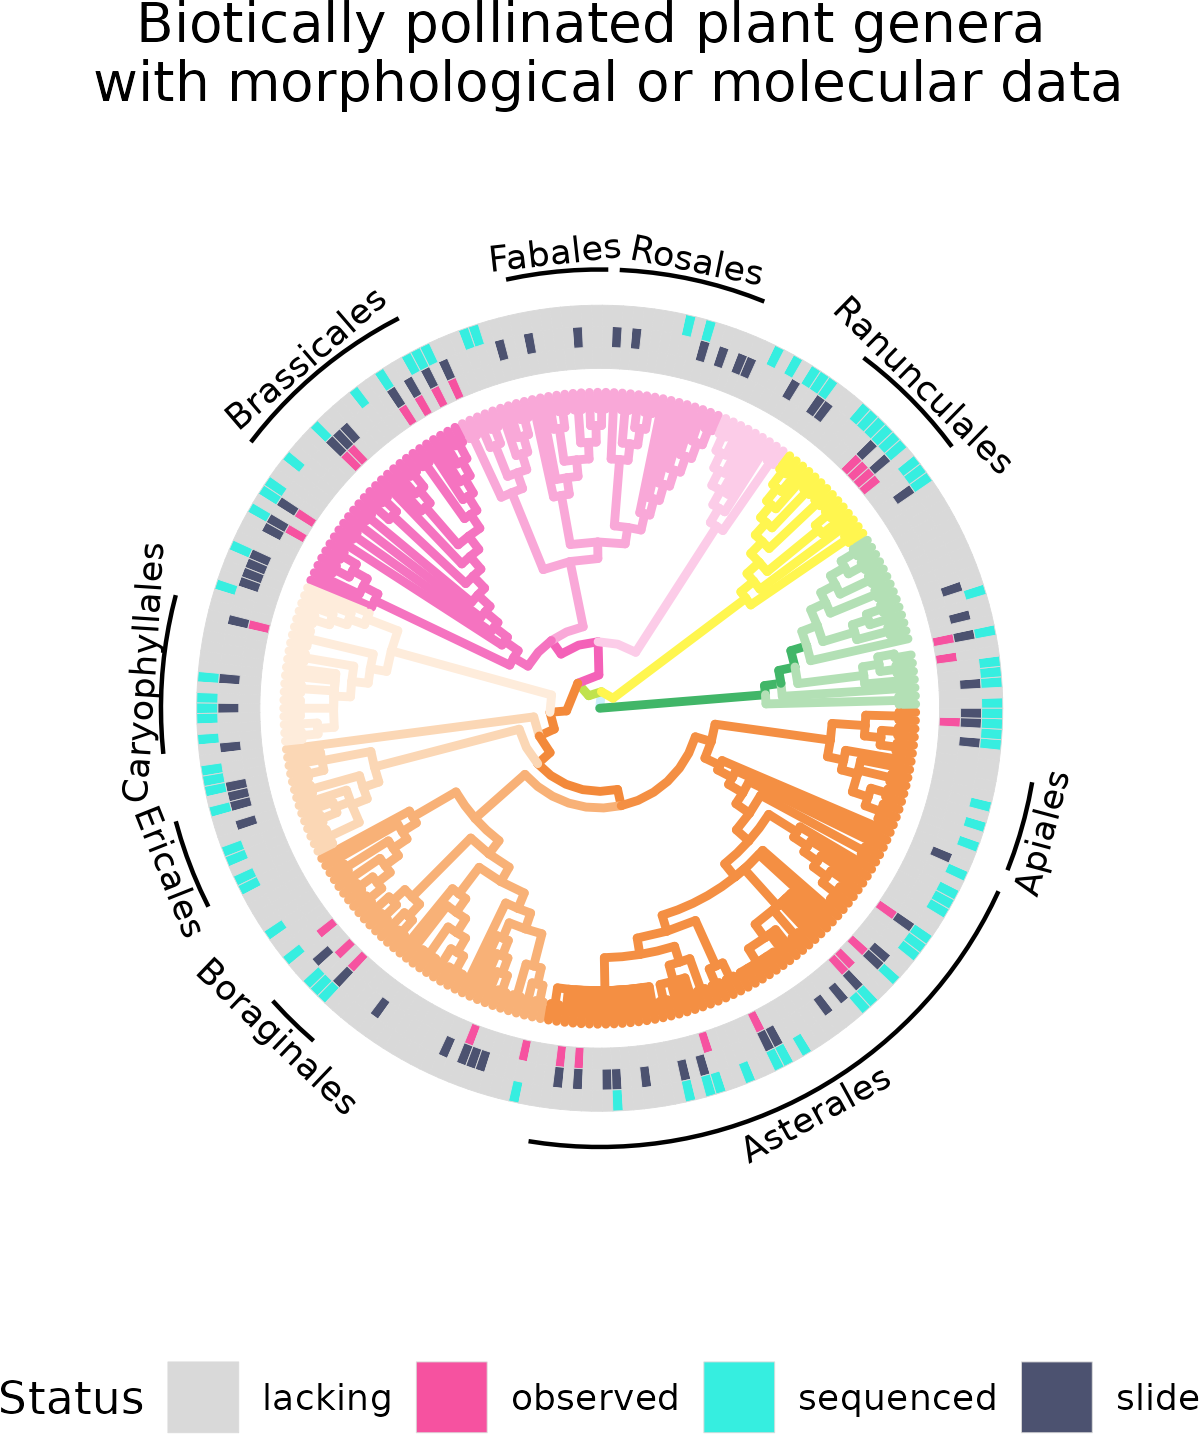
\includegraphics[width=0.65\linewidth]{../graphics/plots/rmbl_draft_tree} \caption{Phylogenetic tree of all biotically pollinated plant genera in the study area. The innermost ring indicates every genus which Queen Bee's were observed to visit. The intermediate ring indicates that at least a single morphological pollen voucher slide was prepared for a member of the genus. The outermost ring indicates that sequence data were available for at least a member of that genus. Branch colors follow APG 4.}\label{fig:Sequence and Morphological Vouchers}
\end{figure}

\hypertarget{metabarcoding-pollen-identification}{%
\subsubsection{3.3 \textbar{} Metabarcoding Pollen
Identification}\label{metabarcoding-pollen-identification}}

\hypertarget{temporal-analysis}{%
\subsubsection{3.3.2 \textbar{} Temporal
Analysis}\label{temporal-analysis}}

The first date of modeled snow melt in the Gothic area (n = 17,
\(\bar{x}\) = 137.9, Mdn = 135, 3\textsuperscript{rd} quartile = 151),
and the first date of a consistent winter snow base (n = 17, \(\bar{x}\)
= 299.9, Mdn = 300, 1\textsuperscript{st} quartile = 291) from
2000-2017, were used as delimiters for the inclusions of herbarium
records in modelling. Of the 439 species predicted likely present in the
area via logistic regression, 332 species (64.4\%) with more than 10
records in the focal level 4 ecoregions (\(\bar{x}\) = 35.016, Mdn = 35,
max = 96) had Weibull estimates calculated, an additional 56 species
(11.2\%) with enough contributing records from the ``Sedimentary
Mid-Elevation Forests'', a large ecoregion generally just beneath the
elevation bands occupied by the five ecoregions around the study area
had Weibull estimates also calculated (\(\bar{x}\) = 13.868, Mdn = 13,
max = 24).

Only 58 of these 388 species (n = 34.6, Mdn = 31) were able to be
compared to plot based observational data from the long term
(1974--2012) data set (CaraDonna \emph{et al.}
(\protect\hyperlink{ref-caradonna2014shifts}{2014})). Of these species
relatively high accord was observed between the long-term ground truthed
data set, and the modelled species. There was very strong evidence that
the Weibull estimates were positively associated with the observed onset
(p \textless{} 0.0001, tau = 0.61), peak (p \textless{} 0.0001, tau =
0.65), and cessation of flowering (p \textless{} 0.0001, tau = 0.49).
There was moderate evidence that the Weibull estimates had a weak
positive association with the observed duration of flowering (p = 0.58,
tau = 0.17).

Of the previous 58 species compared, 47 of these could be compared to
transect based data from the six sites observed in 2015. Due to
methodological differences, the peak flowering was not compared, and due
to the low performance of attempts to model `duration' in the previous
step it was also not compared. There was very strong evidence that the
Weibull estimates were positively associated with the observed onset (p
\textless{} 0.0001, tau = 0.58), and cessation of flowering (p
\textless{} 0.0001, tau = 0.40).

\begin{figure}
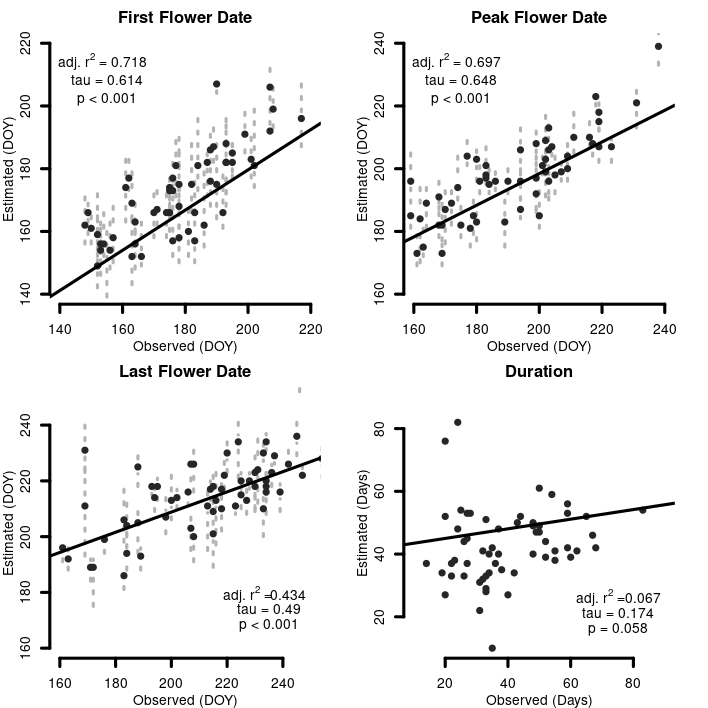
\includegraphics[width=1\linewidth]{../graphics/plots/phenology_estimates_10_90} \caption{Modelled dates of when major flowering events occurred compared between long term and modelled data}\label{fig:plot phenology estimates}
\end{figure}

\begin{figure}
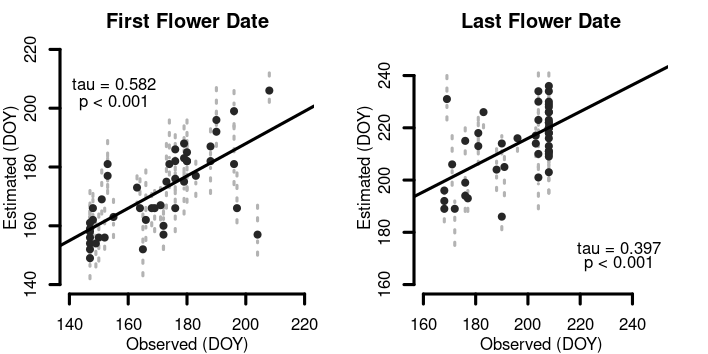
\includegraphics[width=1\linewidth]{../graphics/plots/phenology_estimates-jeo_10_90} \caption{Modelled dates of when major flowering events occurred compared between 2015 and modelled data}\label{fig:plot phenology estimates JEO}
\end{figure}

\hypertarget{molecular-analysis-of-corbiculae-loads}{%
\subsection{3.3.1 \textbar{} Molecular analysis of corbiculae
loads}\label{molecular-analysis-of-corbiculae-loads}}

The 54 corbiculae loads had DNA extracted and underwent various steps
towards hyb-seq, in the end a total of 44 corbiculae samples were
sequenced, 7,752,353 reads were recovered from sequencing. The number of
reads per sequence varied widely (range = 76 - 508,795, \(\bar{x}\) =
176,189.8, Mdn = 138,395). Of the possible 353 loci, the number which
were recovered from each sample, and informative to BLAST were range =
24 - 353, \(\bar{x}\) = 305.5, Mdn = 331. The number of reads per loci
from across all samples had a range of 178 - 506,653, \(\bar{x}\) =
20,688, Mdn = 12,616. \textbf{APPENDIX X Reads Per Loci}.

After trimming 7,865,680 sequences remained. 10,682,538 reads were
matched using Kraken, of the reads classified by Kraken 10,160,768 reads
were matched using Bracken, of the reads classified by Kraken 7,549,608
reads were matched using BLAST. Based upon subjective review of the
three classifiers \textbf{APPENDIX X MOLECULAR NETWORKS - 3 DIFFERENT
ONES}, BLAST was chosen as the classification method which yielded the
most probable results by the field ecologist, and its values were used
for all subsequent analyses.

\begin{table}

\caption{\label{tab:Read Post Processing}Post classification of Sequences via Taxonomy and Ecology,
top 15 most abundant reads}
\centering
\begin{tabular}[t]{c|c|c|c|c}
\hline
Condition & No. Class. & Prcnt. Class. & Total Seqs & Rank\\
\hline
\cellcolor{gray!10}{A} & \cellcolor{gray!10}{143} & \cellcolor{gray!10}{21.0} & \cellcolor{gray!10}{32.0} & \cellcolor{gray!10}{Species}\\
\hline
B & 205 & 30.1 & 10.5 & Species\\
\hline
\cellcolor{gray!10}{C} & \cellcolor{gray!10}{5} & \cellcolor{gray!10}{0.7} & \cellcolor{gray!10}{0.4} & \cellcolor{gray!10}{Genus}\\
\hline
G & 29 & 4.3 & 7.8 & Species\\
\hline
\cellcolor{gray!10}{H} & \cellcolor{gray!10}{280} & \cellcolor{gray!10}{41.2} & \cellcolor{gray!10}{47.9} & \cellcolor{gray!10}{Genus}\\
\hline
None met & 18 & 2.6 & 1.4 & Multiple\\
\hline
\end{tabular}
\end{table}

The initial classification of sequences which were made by BLAST were
reviewed programmatically, using predicted presence of the species (from
spatial modelling), modelled flowering time (from temporal modelling),
and taxonomy (from existing sources). A sequential process was utilized
which reassigned sequences based on binary combinations of the factors
above (Appendix XX). Given the relative sparsity of the number, and
relatedness, of species represented in the sequence database this was
performed to: 1) Identify locally present species represented by
surrogates in the DB 2) Reduce false classifications of focal species 3)
Identify high confidence sequence matches. Of the top ten taxa which
were identified by BLAST for the 680 distinct records, 55.4\% of the
reads were classified to a species representing 48.3\% of all classified
reads, 41.9\% of the reads were classified to genus representing 48.3\%
of all classified reads, and 0\% of the records were classified to
family.

Of the 0 classifications which were assigned to genera without any
species predicted by spatial analyses, were investigated by hand after
post-processing steps. These were all assigned via post-processing
conditions (: , APPENDIX XX). These were manually assigned to a variety
of ranks, occasionally to genus - 0, and species - 0, by consultation of
the alpha-taxonomic literature (Sadeghian \emph{et al.}
(\protect\hyperlink{ref-sadeghian2015molecular}{2015}), Sennikov \&
Kurtto (\protect\hyperlink{ref-sennikov2017phylogenetic}{2017}), Rabeler
\& Wagner (\protect\hyperlink{ref-rabeler2016new}{2016}), Pusalkar \&
Singh (\protect\hyperlink{ref-pusalkar2015taxonomic}{2015}), Moore \&
Bohs (\protect\hyperlink{ref-moore2003its}{2003}), Weber
(\protect\hyperlink{ref-weber1998new}{1998})).

To determine at which level species in pollen loads could be detected
the results of light microscopy were compared to the molecular results.
The pollen samples contained three morphotypes which could readily be
identified via microscopy. Two of these mapped to the clades
(Boraginaceae \& Heliantheae Alliance), and one to a Asteraceae less
Heliantheae. Boraginaceae grains were detected in 92.3\% of samples
where the proportion of target grains were between 0.01-1 (n = 13 Mdn =
0.663). Asteraceae type 1, non-helianthoids, were detected in 50\% of
samples where the proportion of target grains were between 0.001-0.01 (n
= 4 Mdn = 0.001) Asteraceae type 2, Helianthoids, were detected in
33.3\% of samples where the proportion of target grains were between
0.001-0.01 (n = 6 Mdn = 0.005); however, Asteraceae were detected in
80\% of samples where the proportion of target grains were between
0.001-0.01 (n = 10 Mdn = 0.003). Both morphotypes of Asteraceae pollen
were detected in 100\% of samples where the proportion of target grains
were between 0.01-1 (n = 2 Mdn = 0.338).

\includegraphics{manuscript_MEE_files/figure-latex/Correlation between Number of Grains and Number of Sequences-1.pdf}

To detect whether the sequencing reads were semi-quantitative the subset
of all pollen morphotypes distinguishable by microscopy were compared to
the sequence reads. In all instances sequence reads were pooled to the
highest taxonomic rank associated with the morphotype, e.g.~if both
species of \emph{Mertensia} Huth, or one species and read only
classified to genus were present in a sample, the reads were summed. The
total percentage of the ten most abundant grains per sample were then
were then relativized to constitute the entire sample.

The relationship between the number of pollen grains in a sample and the
number of sequence reads is roughly linear, where grains which are
present in trace amounts are overestimated by sequence counts, while
grains present in high amounts are underestimated. This is likely due to
the proportion of high false positives which occur in the classification
process with next-generation sequencing (Bell \emph{et al.}
(\protect\hyperlink{ref-bell2021comparing}{2021})). There was evidence
of a strong correlation between the proportion of grains per morphotype
and the number of sequences per group (0.426, p \textless{} 0.0001, n =
32).

To ascertain the extent to which records of multiple species in a
family, which were suspected to be sampling artefacts occurred in
molecular samples an index of similarity, ala Jaccard, the affinity
index was used to assess co-occurrence (Mainali \emph{et al.}
(\protect\hyperlink{ref-mainali2022better}{2022}), Mainali \& Slud
(\protect\hyperlink{ref-mainali2022alpha}{2022})). Numerous taxa from
the family Ranunculaceae Jussieu (\emph{Caltha} L. sp.,
\emph{Thalictrum} L. spp., \emph{Trollius} L. sp., \emph{Aquilegia} L.
spp.), had \(\alpha\) scores which indicated that they are only present
when a more common confamilial taxa \emph{Delphinium barbeyi} (Huth)
Huth \emph{nuttallianum} Pritz. were recorded. A similar relationship
was observed in the Hydrophyllaceae R.Br. with samples placed in
\emph{Nemophila} Nutt., which only occurred when the more abundant
\emph{Hydrophyllum} L. species were present. The size of flower of
\emph{Nemophila breviflora} A. Gray make it unlikely to be visited by
Bumble Bees, and it is a false positive. The floral morphology and
orientation of flower of \emph{Thalictrum} spp. also makes them unlikely
to be visited, and while evidence of visits to \emph{Caltha} and
\emph{Trollius} are lacking, due to the association between the reads
these results appear unlikely.

\hypertarget{integrated-observational-molecular-and-palynological-network}{%
\subsection{3.6 \textbar{} Integrated Observational, Molecular, and
Palynological
Network}\label{integrated-observational-molecular-and-palynological-network}}

While the spatial results were used to declare the taxonomic composition
of the sequence database, temporal results were used in consideration
with plant phylogeny to retroactively, reassign the assignment of
sequences to taxa. Essentially, if a sequence was identified to a taxon
which was not known from the field site

For example a many sequences which mapped to the Asteraceae family, but
which was flagged by temporal filters and is present in both \emph{B.
nevadensis} Cresson and \emph{B. rufocinctus} Cresson pollen is most
likely \emph{Frasera} Walter, which failed extractions for the reference
library failed (APPENDIX XX). A similar likely mismatch could be between
what was fide molecular evidence as \emph{Agastache pallidiflora} (A.
Heller) Rydb. but where feeding was infrequently observed on
\emph{Pedicularis} L., likely due to this entire order being represented
by only a single molecular reference species.

\includegraphics{manuscript_MEE_files/figure-latex/compare results-1.pdf}

\begin{verbatim}
## 
##  Wilcoxon rank sum test with continuity correction
## 
## data:  pull(ACC_sens_Spec[ACC_sens_Spec$Method == "COMP", "Sp_Acc"]) and pull(ACC_sens_Spec[ACC_sens_Spec$Method == "BLAST", "Sp_Acc"])
## W = 1254.5, p-value = 5.367e-06
## alternative hypothesis: true location shift is greater than 0
\end{verbatim}

\includegraphics{manuscript_MEE_files/figure-latex/compare results-2.pdf}

Situations where SDM's led to incorrect results at the species level are
evident with classification to \emph{Scabrethia Scabra} (Hooker) W.A.
Weber, this match almost certainly representing \emph{Wyethia arizonica}
A. Gray (Weber (\protect\hyperlink{ref-weber1998new}{1998})), a taxon
known to be visited by queen bee's via our floral observations. An
expected inaccuracy of the classification scheme is in genus level
placements, e.g.~were \emph{Epilobium} L. (Onagraceae Juss.) spp. were
classified. However, given the small size of their flowers in the study
area, these results more likely indicate that a species of
\emph{Chamaenerion} Seg. (a segregate genus) such as \emph{C.
angustifolium} (L.) Scop. or \emph{latifolium} (L.) Sweet is
occasionally utilized, as it supported by limited palynology data. An
issue with reclassification within the family level in combination with
time included reclassifying \emph{Parnassia palustris} L. to
\emph{Paxistima myrsinites} (Pursh) Rafinesque. However, based on flower
size it is more likely that the visited taxon was \emph{P. palustris}.

Regarding limitations of morphological data we suspect that there were
two morphotypes of pollen identified as Ericaceae Juss. were actually
Onagraceae (Samples 19 \& 44), based on molecular results.

It is not unlikely that much of the difference in the results between
the observational and molecular work are attributable to the challenges
in detecting rare events in these smaller sizes. For example, no more
than 10 bee corbiculae loads per species were sequenced with the Mdn =
5.5 \ldots{} , and the median of interactions with the top 5 plant sizes
constituted 0.8283385 of the top interactions.

Accordingly, combining the results of floral observations, and
palynology, molecular sequencing - both pre and post processing, we
subjectively developed re-classifications of the contents of pollen
grains\ldots{}

\hypertarget{discussion}{%
\section{4 \textbar{} DISCUSSION}\label{discussion}}

We have demonstrated how the Angiosperms533 hyb-seq probes may be used
for plant barcoding in a metagenomic context (Johnson \emph{et al.}
(\protect\hyperlink{ref-johnson2019universal}{2019}), Hollingsworth
\emph{et al.} (\protect\hyperlink{ref-hollingsworth2016telling}{2016})).
This was exemplified in an ecologically relevant scenario, where the
results have immediate implications for natural history guided
fundamental science and land management. The test pollen loads contained
a number of closely related taxa, some in notoriously morphologically
difficult clades with rapid rates of diversification
(e.g.~\emph{Mertensia}, \emph{Lupinus} L.), at naturally occurring
proportions (Nevado \emph{et al.}
(\protect\hyperlink{ref-nevado2016widespread}{2016}), Nazaire \& Hufford
(\protect\hyperlink{ref-nazaire2014phylogenetic}{2014})). We
incorporated spatial and temporal approaches for creating custom
sequence databases an approach which is readily applicable to any lab
group with the capacity to perform next-generation sequencing across the
entirety of multiple continents, and which we expect to be highly
beneficial in many study areas. By combining insights from these novel
approaches with an extensive observational field based study we show how
these methods may be applied to test a variety of hypotheses related to
ecological interactions.

The SDM's which we generated, with relatively few occurrence records and
few modelling iterations, performed beyond expectations, likely due to
the utility of the predictor variables and strong alignment of
vegetation by orographic precipitation in the study area. However, we
had difficulties in evaluating our predictions in an operational
context. We utilized the database query approach, to only model species
with a high probability of not being dispersal limited to the focal
area, and focused on a relevant subset of many of these species ranges
to reduce the contributions of range wide adaptions on habitat (Sork
(\protect\hyperlink{ref-sork2018genomic}{2018}), Joshi \emph{et al.}
(\protect\hyperlink{ref-joshi2001local}{2001})). While the models worked
well compared to both test, and validation with external point data,
moving from points to polygon features was more difficult. We were able
to compare our results to 1) a Flora, 2) lists of plants used by Bumble
Bees at plots; the former inappropriate in that it contained a great
number of species which we sought to use modelling to reduce \emph{e.g.}
all strictly alpine species, and the latter inappropriate in that it
contained only species relevant to \emph{Bombus} but had no official
`absence' data. Further given the, size of the minimum spanning tree
which we extracted points to, a formal floristic inventory would still
be a time intensive process. Accordingly, we expect the real results of
our data lay somewhere in between these two evaluations; with an excess
of species predicted present (Dubuis \emph{et al.}
(\protect\hyperlink{ref-dubuis2011predicting}{2011}), Calabrese \emph{et
al.} (\protect\hyperlink{ref-calabrese2014stacking}{2014}),
Pinto-Ledezma \& Cavender-Bares
(\protect\hyperlink{ref-pinto2021predicting}{2021})), but few enough
that they lend themselves to metabarcoding. We observe that our models
seemed very capable of effectively identifying alpine species and
removing them in binomial contexts. Difficulties in temporal models
related to variability in drivers of flowering phenology. AND SMALL
SAMPLE SIZE

These results show that the overall results between \textbf{Bumble Bee
ecology} observational and barcoding are largely congruent. But that
\ldots{} We analyzed pollen loads from all of the most common bumble bee
species in the area (Pyke (\protect\hyperlink{ref-pyke1982local}{1982}))
Future analyses of the long term data set\ldots{}

Results from palynological analyses show that several species of bee
show near perfect fidelity to the genus \emph{Mertensia} on a per visit
basis\ldots{} General results show high congruence between foraging and
molecular results, indicating that concerns regarding mismatch between
observational networks need not persist with \emph{Bombus}
studies\ldots{}

Some foraging preferences of \emph{Bombus}, both at this field site and
across a great many localities globally emerge from this work, which
reiterates the needs for land managers to maintain relatively high
amounts of members of the Fabaceae, Boraginaceae, and Ranunculaceae, in
Western North American montane landscapes (Goulson \emph{et al.}
(\protect\hyperlink{ref-goulson2005causes}{2005}), Goulson
(\protect\hyperlink{ref-goulson2010bumblebees}{2010}), Liang \emph{et
al.} (\protect\hyperlink{ref-liang2021evolutionary}{2021}), Bontsutsnaja
\emph{et al.} (\protect\hyperlink{ref-bontvsutvsnaja2021bumble}{2021})).
Numerous historic, and some ongoing, land management practices reduce
the ability of many landscapes to support stable populations of
\emph{Bombus}. Historic livestock grazing was often associated with the
targeted removal of many species of plants which are known to have
compounds toxic to cattle. In particular, the removal of locoweeds
(Fabaceae: \emph{Astragalus} L. \& \emph{Oxytropis} DC.) and larkspurs
(Ranunculaceae: \emph{Delphinium}) were common across public lands
administered by the United States Forest Service (Ralphs \& Ueckert
(\protect\hyperlink{ref-ralphs1988herbicide}{1988}), Aldous
(\protect\hyperlink{ref-aldous1919eradicating}{1919}), Ralphs \emph{et
al.} (\protect\hyperlink{ref-ralphs2003mechanism}{2003})). Further
actions, generally initiated by early settlers, involved the
channelization and incising of streams, culling of beavers, and leaving
cattle concentrated on higher order stream banks for significant periods
of time, all processes which lower the water tables and reduced the
extent of stream-associated {[}riverine{]} wetlands and the mesic
meadows fringes which provide habitat for many species of tall
\emph{Mertensia} (Boraginaceae, e.g.~\emph{M. ciliata} Torr. G. Don.)
widely distributed across Western North America, and to an extent
\emph{Delphinium barbeyi} and many species of native \emph{Trifolium} L.
(Dahl (\protect\hyperlink{ref-dahl1990wetlands}{1990}), Naiman \emph{et
al.} (\protect\hyperlink{ref-naiman1988alteration}{1988}), Belsky
\emph{et al.} (\protect\hyperlink{ref-belsky1999survey}{1999}), Cooke \&
Reeves (\protect\hyperlink{ref-cooke1976arroyos}{1976})). Fire
suppression further resulted in the succession of many Aspen
(\emph{Populus tremuloides} Michx.) groves to Conifer stands, decreasing
the mosaic of age structured habitats in many landscapes, adversely
effects habitat for tall \emph{Mertensia} species and several species of
\emph{Delphinium} (Brewen \emph{et al.}
(\protect\hyperlink{ref-brewen202176}{2021}), Keane
(\protect\hyperlink{ref-keane2002cascading}{2002})). Finally the effects
of Nitrogen deposition, especially given the West's rapidly growing
population still pose adverse effects on the abundance of a variety of
species of Fabaceae at Urban-Rural interfaces (see Stevens \emph{et al.}
(\protect\hyperlink{ref-stevens2018atmospheric}{2018}), Fenn \emph{et
al.} (\protect\hyperlink{ref-fenn2003ecological}{2003})). Current
solutions to these issues, involve targeted burns, reintroduction of
beavers and beaver habitat analogs, and the possibility of re-seeding a
variety of `locoweeds' and `larkspurs' in areas now seldom used, or only
used for early, grazing. The highly enthusiastic response of land
managers, and homeowners, to plant \emph{Ascelpias} L., using
genetically appropriate materials, to improve Monarch Butterfly
(\emph{Danaus plexippus} L.) habitat provides an effective framework for
the latter (Oberhauser \emph{et al.}
(\protect\hyperlink{ref-oberhauser2015monarchs}{2015}), Basey \emph{et
al.} (\protect\hyperlink{ref-basey2015producing}{2015})).

We have concerns regarding the number of persons training to become and
practice botany, and grave concerns regarding the funding mechanisms for
floristic and field based botanical research and for centralized
authorities to produce consensus opinions on alpha taxonomy (Prather
\emph{et al.} (\protect\hyperlink{ref-prather2004decline}{2004b}),
Kramer \& Havens (\protect\hyperlink{ref-kramer2015report}{2015}),
Prather \emph{et al.}
(\protect\hyperlink{ref-prather2004implications}{2004a}), Crisci
\emph{et al.} (\protect\hyperlink{ref-crisci2020end}{2020}), Manzano
(\protect\hyperlink{ref-manzano2021flippant}{2021}), Stroud \emph{et
al.} (\protect\hyperlink{ref-stroud2022botanical}{2022})). To reduce the
effects of a low population density of botanists on the maintenance of
and production of Flora's and to foster meta-genomics across landscapes
without field stations we utilized Species Distribution Modelling to
generate predictive species lists. In this proof-of-concept example we
performed several iterations of modelling runs, and several approaches
(i.e.~the `linear models', and the `machine learning'), which took
notable amounts of compute power. We suspect the possible deleterious
nature of this endeavor may be reduced by: 1) more field surveying by
crews will reduce the need to generate as many species 2) fewer runs of
models, 3) only running machine learning models which do not require an
explicitly process to reduce spatial autocorrelation. However, given the
time required to perform all aspects of a study, even our amount of
computation was negligible. Further, we are very optimistic about the
possibility for persons to perform these tasks, as mentioned we utilized
roughly only one quarter of the records which were digitally available
for presence, and we suspect others will have enough records to perform
this process nearly anywhere else in the temperate. In certain scenarios
modelling of predicted species via more formally tailored S(tacked)-SDM
or J(oint)-SDM approaches may be beneficial (Wilkinson \emph{et al.}
(\protect\hyperlink{ref-wilkinson2021defining}{2021}), Pinto-Ledezma \&
Cavender-Bares (\protect\hyperlink{ref-pinto2021predicting}{2021}),
Schmitt \emph{et al.} (\protect\hyperlink{ref-schmitt2017ssdm}{2017})).

Tandem to the lack of continued expertise required to generate and
maintain species lists, is the expertise required to continue tracking
when major phenological events occur in many plant species at relatively
fine scales or under novel climates. Knowledge of these events is
currently limited to general time periods of only a handful of
phenological events and groups of organisms (e.g.~flowering initiation,
or trees) (Prather \emph{et al.}
(\protect\hyperlink{ref-prather2004implications}{2004a}), Li \emph{et
al.} (\protect\hyperlink{ref-li2016responses}{2016})). While many
programs and initiatives exist to collect phenological information on
subsets of easily identifiable charismatic species to detect major
trends in phenology, these capture only a subset of the extent diversity
(Betancourt \emph{et al.}
(\protect\hyperlink{ref-betancourt2005implementing}{2005}), Havens
\emph{et al.} (\protect\hyperlink{ref-havens2007chicago}{2007})). In
many instances it appears that while landscapes respond similarly to
environmental variables which predict phenological responses, that
individual species vary widely in their responses to similar
environmental cues, or respond to different cues (Augspurger \& Zaya
(\protect\hyperlink{ref-augspurger2020concordance}{2020}), Xie \emph{et
al.} (\protect\hyperlink{ref-xie2015deciduous}{2015}), Xie \emph{et al.}
(\protect\hyperlink{ref-xie2018predicting}{2018}), CaraDonna \emph{et
al.} (\protect\hyperlink{ref-caradonna2014shifts}{2014})). As can be
seen here, predictions of when a single, major phenological event occurs
is already data limited. A more promising approach for the tropics may
lay in utilizing circular statistics (Park \emph{et al.}
(\protect\hyperlink{ref-park2022herbarium}{2022})).

The nearly complete Plant and Fungal Tree of Life (PAFTOL) will provide
a comprehensive phylogenetic backbone of the entire plant kingdom, and
the inclusion of A353 probes with lineage specific probe sets is common
in producing massive genetic datasets (Baker \emph{et al.}
(\protect\hyperlink{ref-baker2021exploring}{2021b})). We predict that
the A353 probes which it is utilizing to work nearly immediately for DNA
barcoding of whole plant material, and that more elaborate validation
studies in controlled metabarcoding settings, utilizing existing
experimental designs, will have favorable results (Bell \emph{et al.}
(\protect\hyperlink{ref-bell2017applying}{2017}), Bell \emph{et al.}
(\protect\hyperlink{ref-bell2019quantitative}{2019}), Bell \emph{et al.}
(\protect\hyperlink{ref-bell2021comparing}{2021}), Lamb \emph{et al.}
(\protect\hyperlink{ref-lamb2019quantitative}{2019})). In particular the
harvesting of loci with more variation in certain lineages, and or with
more variable flanking regions, will prove promising for identifying
closely related plant material (CITE). We suspect that conserved reaches
of genes resulted in the high amounts of reads in somewhat obscure
species. Given that the A353 loci are nuclear, single copy, and a
variety are present the possibility of identifying target loci for
quantitative purposes is high, without continual PCR enrichment is
possible; this would align with relatively high efficacy of WGS (Lang
\emph{et al.} (\protect\hyperlink{ref-lang2019genome}{2019}), Peel
\emph{et al.} (\protect\hyperlink{ref-peel2019semi}{2019}), Bell
\emph{et al.} (\protect\hyperlink{ref-bell2021comparing}{2021})). Recent
evidence indicates that the potential for identifying nearly cryptic
taxa and even infra-specific inference, of either whole plant material,
and perhaps in metagenomic context are possible (Ottenlips \emph{et al.}
(\protect\hyperlink{ref-ottenlips2021resolving}{2021}), Wenzell \emph{et
al.} (\protect\hyperlink{ref-wenzell2021incomplete}{2021}), Loke et
al.~in prep, Slimp \emph{et al.}
(\protect\hyperlink{ref-slimp2021potential}{2021}), Beck \emph{et al.}
(\protect\hyperlink{ref-beck2021palmer}{2021})). We further believe that
in synthetic phylogenetic trees - with incorporation of NGS backbones -
will allow in automatic reassignment of reads as a function of
phylogenetic distance with measures of uncertainty (Hinchliff \emph{et
al.} (\protect\hyperlink{ref-hinchliff2015synthesis}{2015}), Smith \&
Brown (\protect\hyperlink{ref-smith2018constructing}{2018}), Baker
\emph{et al.} (\protect\hyperlink{ref-baker2021PAFTOL}{2021a})).

\hypertarget{conclusion}{%
\section{5 \textbar{} CONCLUSION}\label{conclusion}}

We believe that the combination of spatial and temporal models, united
and guided by localized natural history knowledge, provides the
essential components of a bayesian framework for approaching the coarse
elucidation of ecological interactions using DNA Barcoding. Herein we
crudely utilized this thinking via binary outcomes, should a species
predicted be predicted present or not? Is it unequivocally flowering or
not? Myriad data show biological systems and ecological interactions
have more variance than can be reasonably discretely parsed. We expect
that within a bayesian framework studies of pollinator behavior may be
enacted via this approach at a landscape level, e.g.~the scale of an
entire drainage basin such as the Gunnison which is quickly becoming one
of the worlds few model ecosystems. We hope that the promise of A353
probes as tools for metabarcoding play a role in these endeavors.

\textbf{AUTHOR CONTRIBUTIONS:} R.C.B conducted botanical collections,
conducted all molecular lab work, lead all analyses, and writing. J.E.O
conceived, designed, and conducted all ecological fieldwork, assisted
with analyses, and writing. E.J.W. prepared, imaged, and collected trait
data on pollen reference slides, and assisted with analysis of trait
data and writing a dichotomous key. S.T. assisted with spatial analyses
and writing. P.J.C assisted with ecological analyses and writing. J.B.F.
conceived, and designed all lab work, analyses, and integration of
approaches, assisted with writing, and secured funding for molecular
work.

\textbf{ACKNOWLEDGMENTS:} Nyree Zerega for assistance obtaining herbaria
loans and accessioning our collections at CHIC. Pat Herendeen for
assistance with virtually all aspects of preparing pollen vouchers and
the identification process. Hilary Noble, Zoe Diaz-Martinez, Angela
McDonnell, \& Elena Loke for assistance with genomic library
preparation. Ian Breckheimer for sharing the SDM predictor variables. We
thank the curators at the following herbaria for supplying tissue: Ben
Legler at Stillinger (ID), Charles (Rick) Williams at Ray J. Davis
(IDS), (B)Ernie Nelson at Rocky Mountain (RM); and the collectors: D.
Knoke, L. Brummer, J. Boyd, C. Davidson, I. Gilman, M. Kirkpatrick, S.
McCauley, J. Smith, K. Taylor, \& C. Williams. David Giblin \& Mare
Nazaire for sharing relevant sections of an advanced draft of FNA V. 15.
The Bureau of Land Management is thanked as many plant specimens were
collected by R.C.B as a partner or contractor to the agency; Sarah
Burnett and Lauren Price are thanked for sharing AIM data. Sanda and New
England Biotech are gratefully acknowledged for technical support and
generously sharing samples. T.C.H. Cole for sharing the Angiosperm
Phylogeny 4 colour palette. The Program in Plant Biology and
Conservation is thanked for funding. The holdings of the following
herbaria were essential for this project: AK, ALTA, ASU, BABY, BC, BM,
BMO, BOON, BRIT, CANB, CAS, CHSC, CM, CMN, CNS, COLO, CONN, CS, CSU,
DAV, DBG, DES, ENCB, F, FR, G, GH, GZU, IAC, K, KR, KSP, KSTC, KU, LD,
LOB, LSU, MA, MACF, MEL, MICH, MIL, MIN, MNHN, MO, MO, MT, MW, NCSC,
NSW, NY, NYBG, O, OBI, PI, RBG, RSA, SD, SDSU, SFV, TENN, TRT, UA, UAC,
UAM, UAZ, UBC, UBC, UCR, UCS, UCSB, UMO, UNM, UPS, US, USCH, USF, USU,
UTEP, UWBM, V, VT, W, WSCO, WU, XAL, YPM, Z.

\textbf{CONFLICT OF INTERESTS} The authors declare no conflicts of
interest.

\textbf{PEER REVIEW} The peer review history for this document is
available at \ldots{}

\textbf{DATA AVAILABILITY STATEMENT} The queries required to download
all data used in this project are located in\ldots{} All novel
sequencing data are located at NCBI\ldots{}

\textbf{ORCID}

Paul CaraDonna \url{https://orcid.org/0000-0003-3517-9090}\\
Jeremie Fant \url{https://orcid.org/0000-0001-9276-1111}\\
Jane Ogilvie \url{https://orcid.org/0000-0001-8546-0417}\\
Sophie Taddeo \url{https://orcid.org/0000-0002-7789-1417}

\hypertarget{references}{%
\section{References}\label{references}}

\hypertarget{supporting}{%
\section{Supporting}\label{supporting}}

\newpage

Appendix 1 - Site Maps

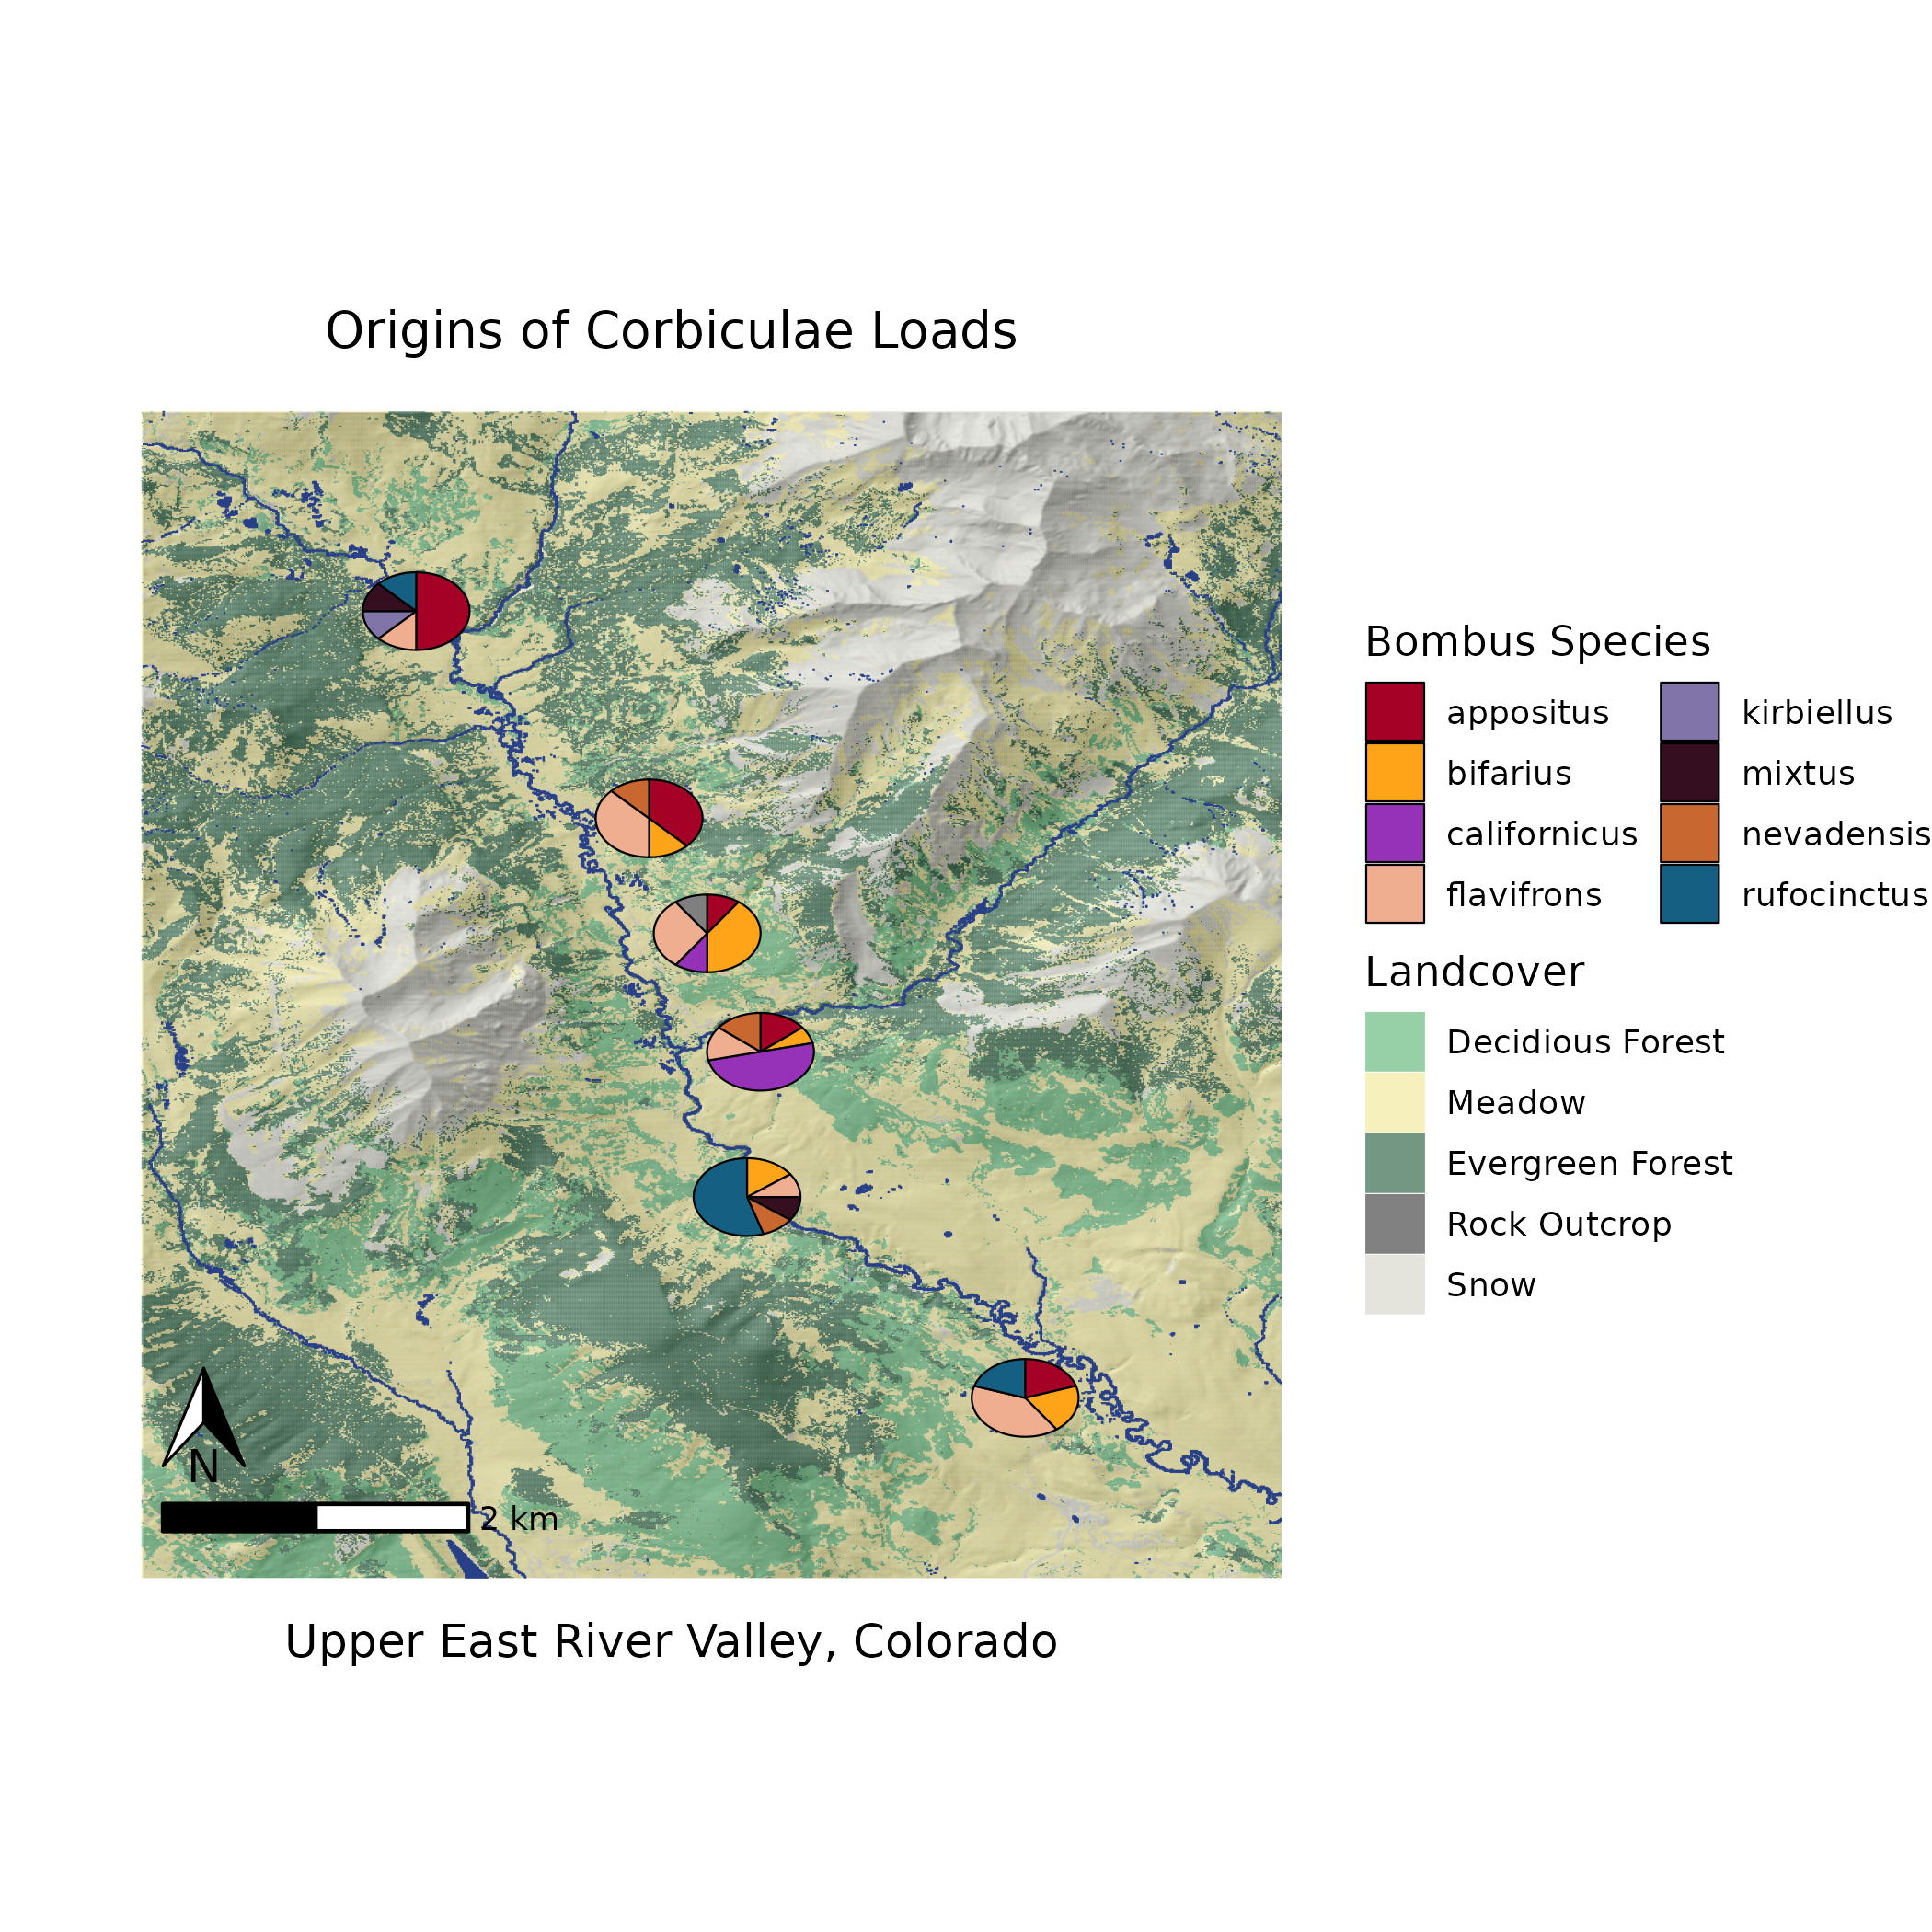
\includegraphics[width=27.01in]{../graphics/plots/siteMaps}

\newpage

Appendix 2 - Species Distribution Models Predictors

\begin{longtable}[]{@{}lccc@{}}
\toprule()
Layer & LM & Description & Source \\
\midrule()
\endhead
1. & N & Mean annual cloudiness - MODIS & Wilson et al.~2016 \\
2. & Y & Cloudiness seasonality 1 - MODIS & Wilson et al.~2016 \\
3. & N & Cloudiness seasonality 2 - MODIS & Wilson et al.~2016 \\
4. & Y & Cloudiness seasonality 3 - MODIS & Wilson et al.~2016 \\
5. & N & Beginning of the frost-free period & Wang et al. \\
6. & N & Climatic moisture deficit & Wang et al. \\
7. & N & Degree-days above 5C & Wang et al. \\
8. & N & Mean annual precipitation & Wang et al. \\
9. & Y & Mean annual precipitation as snow & Wang et al. \\
10. & Y & Temperature seasonality & Wang et al. \\
11. & Y & 2015 Percent Grass/Herbaceous cover - MODIS & (MOD44B) \\
12. & Y & 2015 Percent Tree cover from Landsat 7/8 & (GLCF) \\
13. & Y & Soil probability of bedrock (R Horizon) & SoilGrids \\
14. & N & Soil organic carbon (Tonnes / ha) & SoilGrids \\
15. & N & Surface soil pH in H\textsubscript{2}O & SoilGrids \\
16. & Y & Surface soil percent sand & SoilGrids \\
17. & Y & Soil USDA class & SoilGrids \\
18. & N & Topographic elevation & EarthEnv DEM \\
19. & Y & Topographic elevation, moving window. & EarthEnv DEM \\
20. & Y & Topographic percent slope & EarthEnv DEM \\
21. & Y & Topographic wetness index & EarthEnv DEM \\
22. & Y & Topographic aspect & EarthEnv DEM \\
23. & Y & Annual potential solar radiation computed & r.sun \\
24. & N & Estimated actual (w/-cloud) solar radiation & r.sun / Wilson
et al.~2016 \\
25. & Y & Log-transformed distance to surface water & Global Surface
Water Explorer \\
26. & Y & Percent surface water & Global Surface Water Explorer \\
\bottomrule()
\end{longtable}

\newpage

Appendix 3 - Molecular Reference Specimen Table

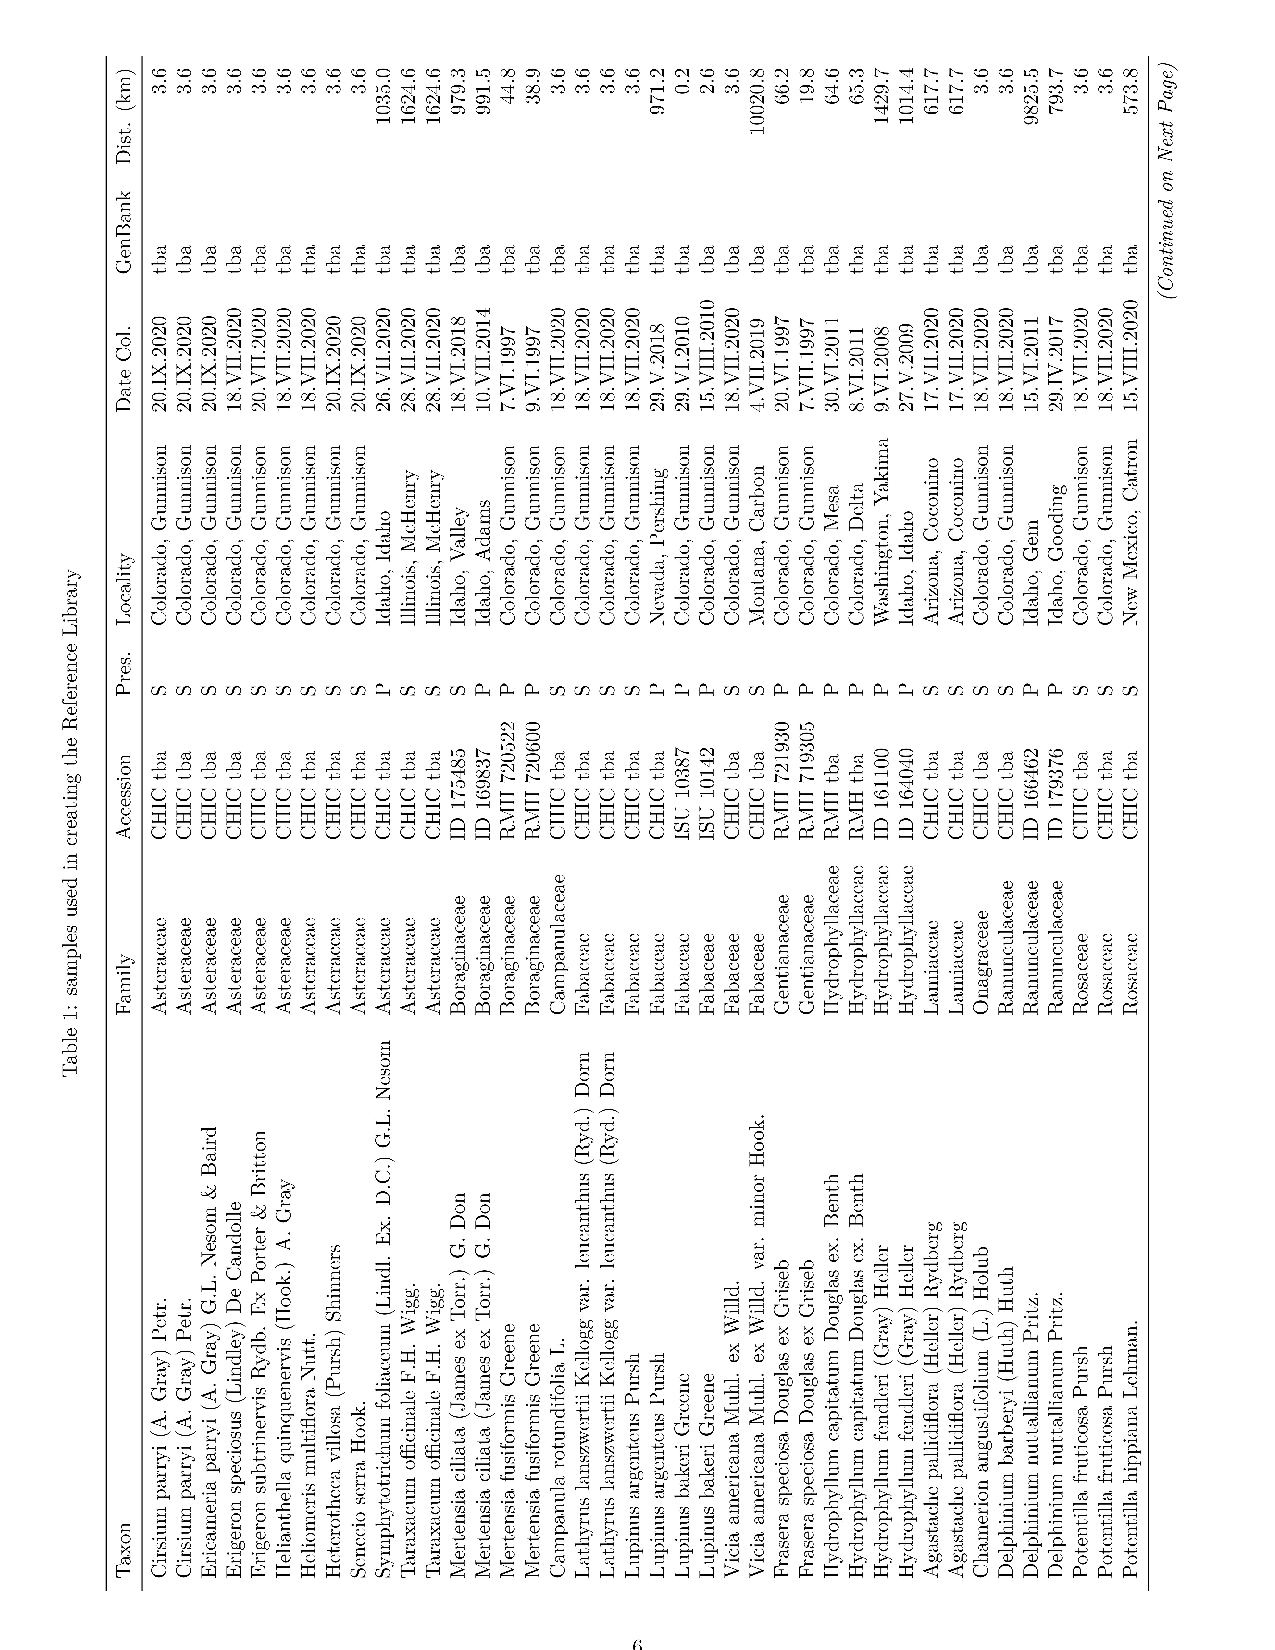
\includegraphics{../graphics/tables/specimen_tables-1.pdf}

\newpage

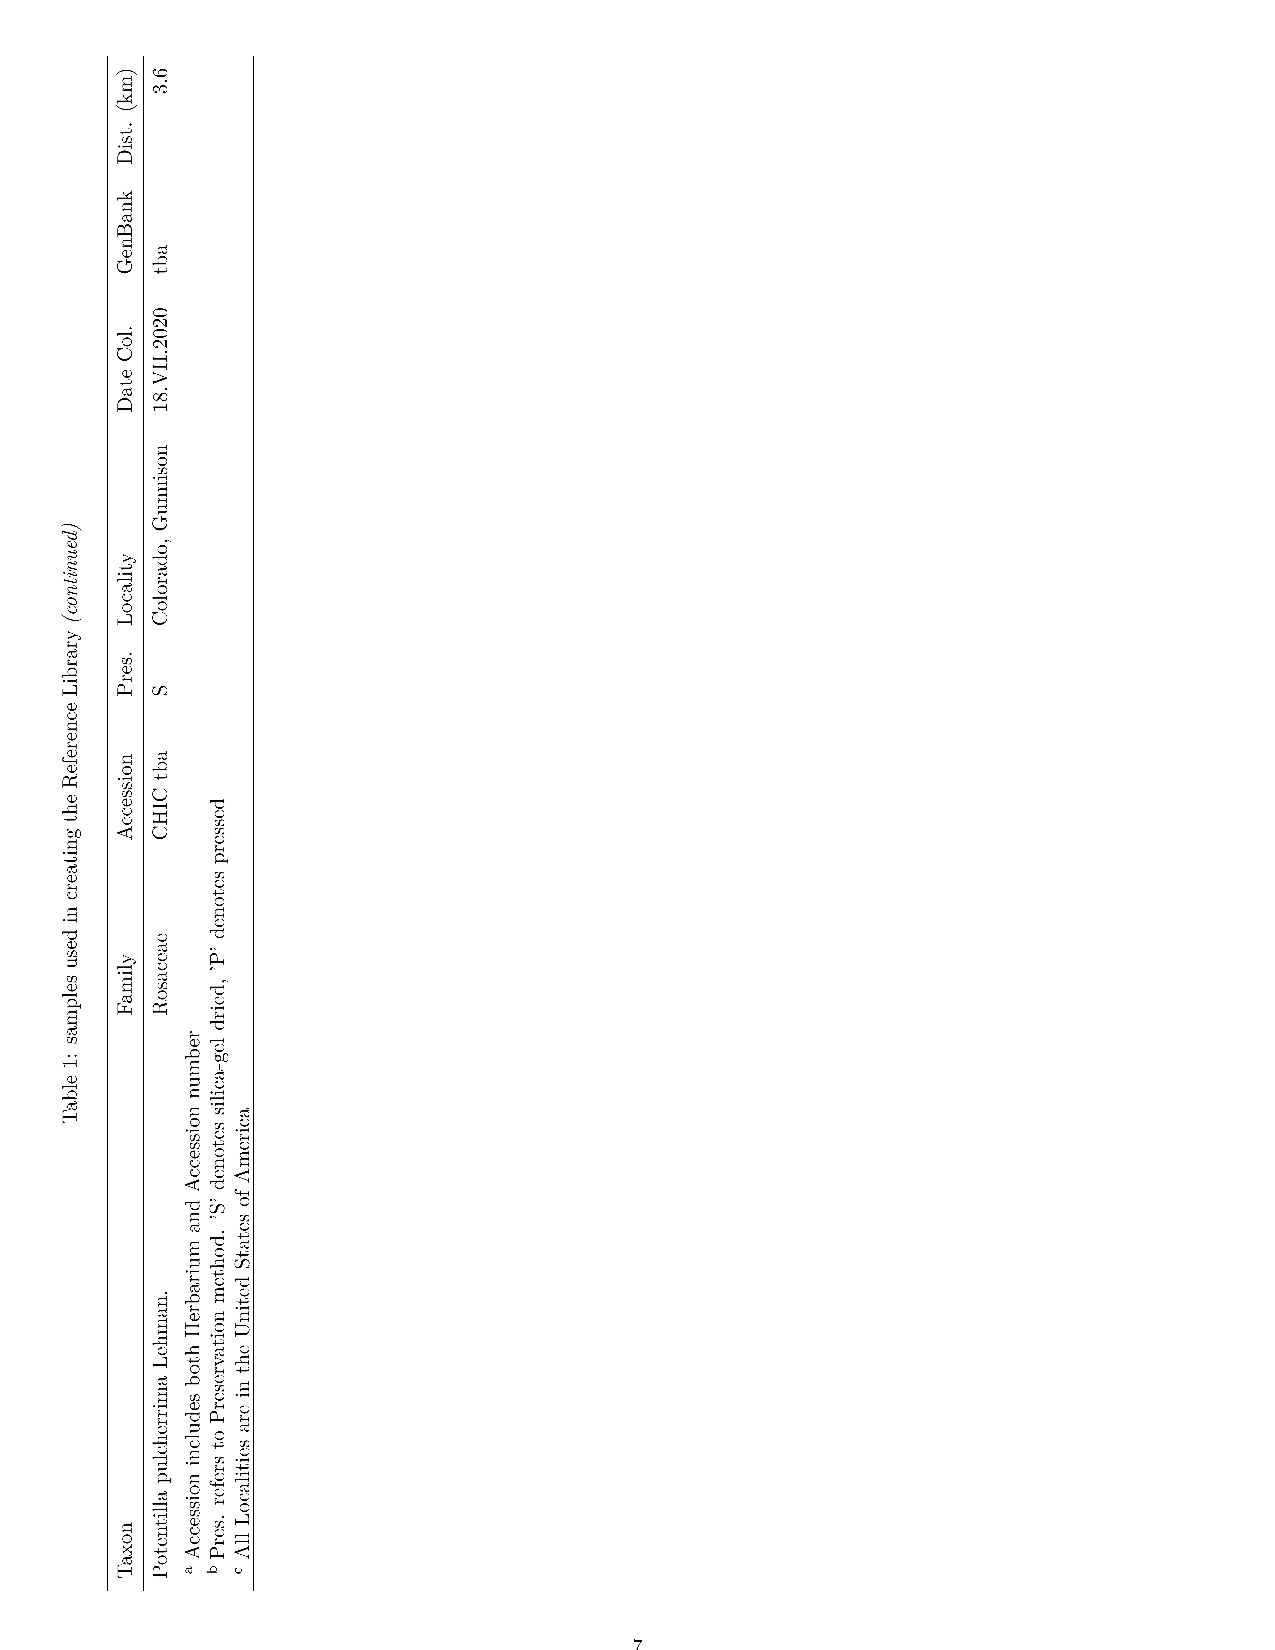
\includegraphics{../graphics/tables/specimen_tables-2.pdf}

\newpage

Appendix 4 - All Pollen Reference Slides Used to Establish Morphotypes

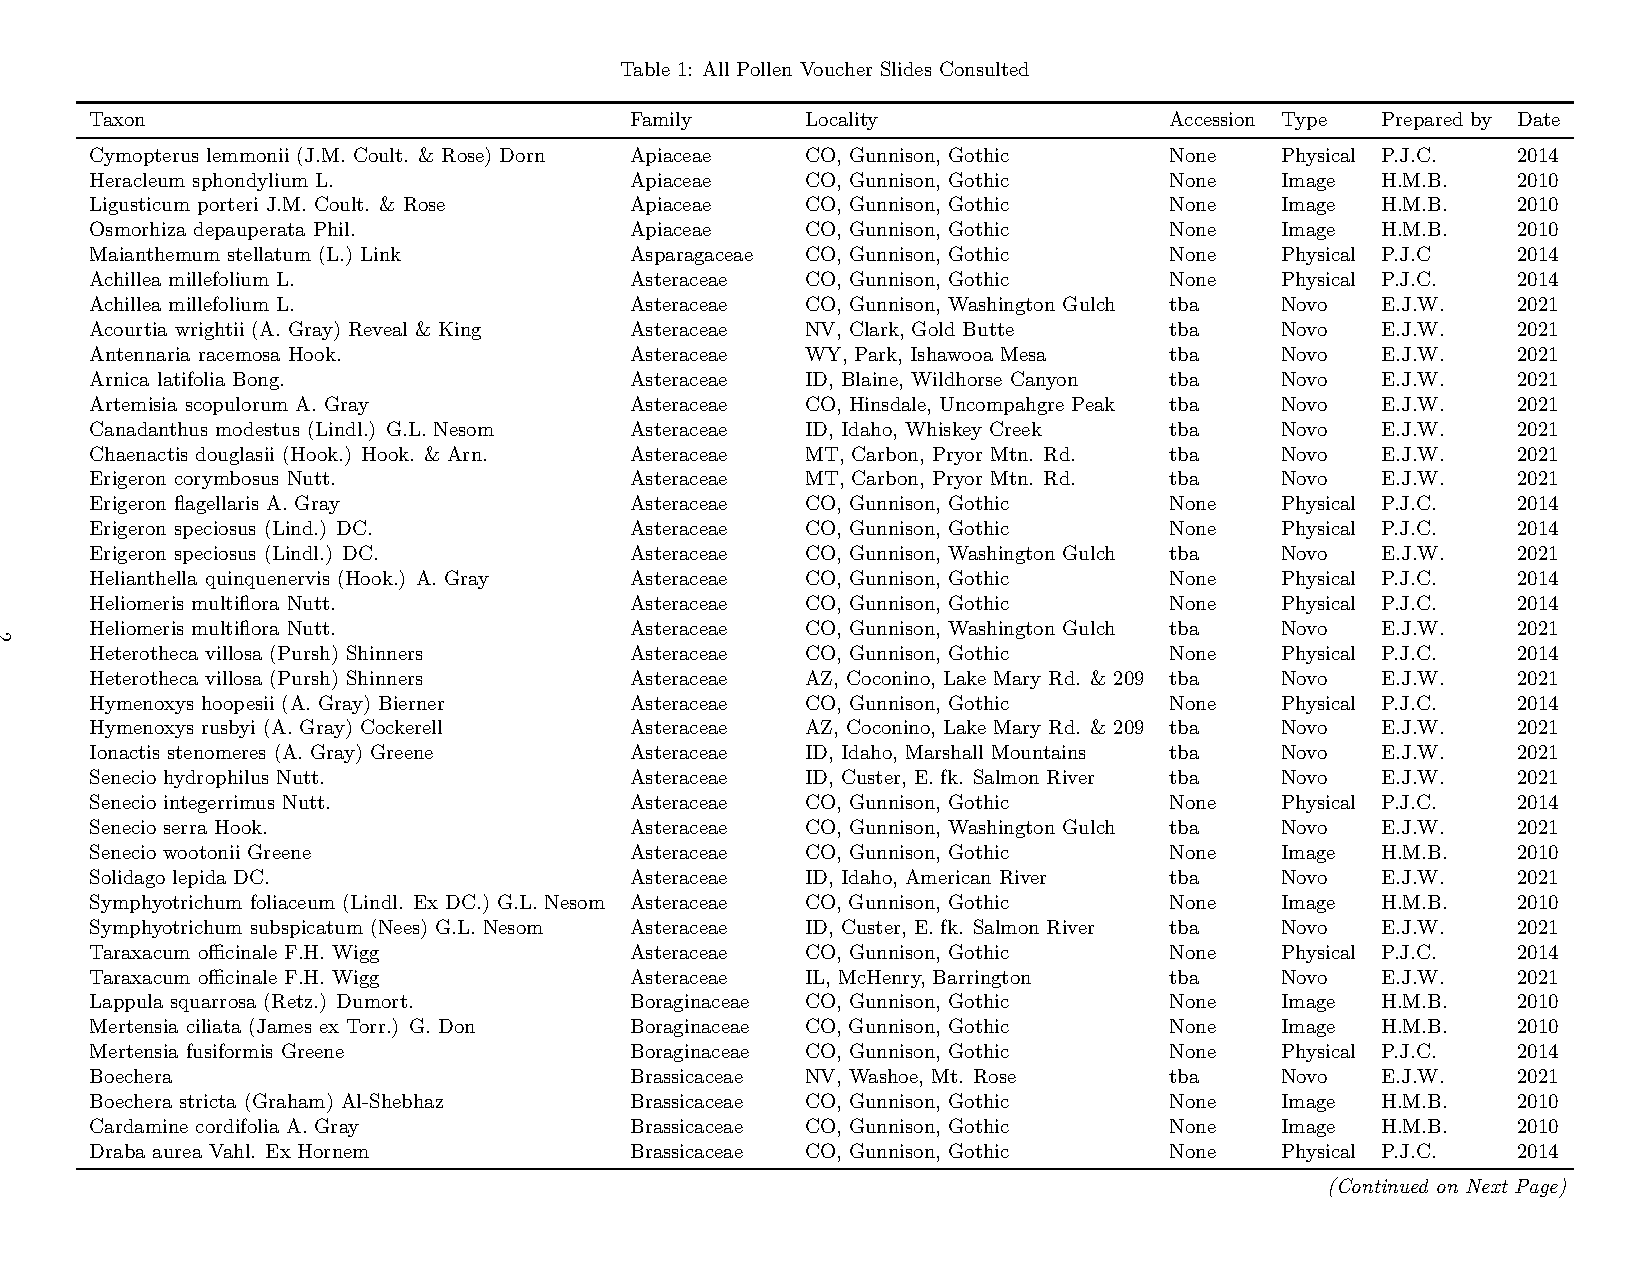
\includegraphics{../graphics/assorted/pollen_slide_table_reduced-1.pdf}

\newpage

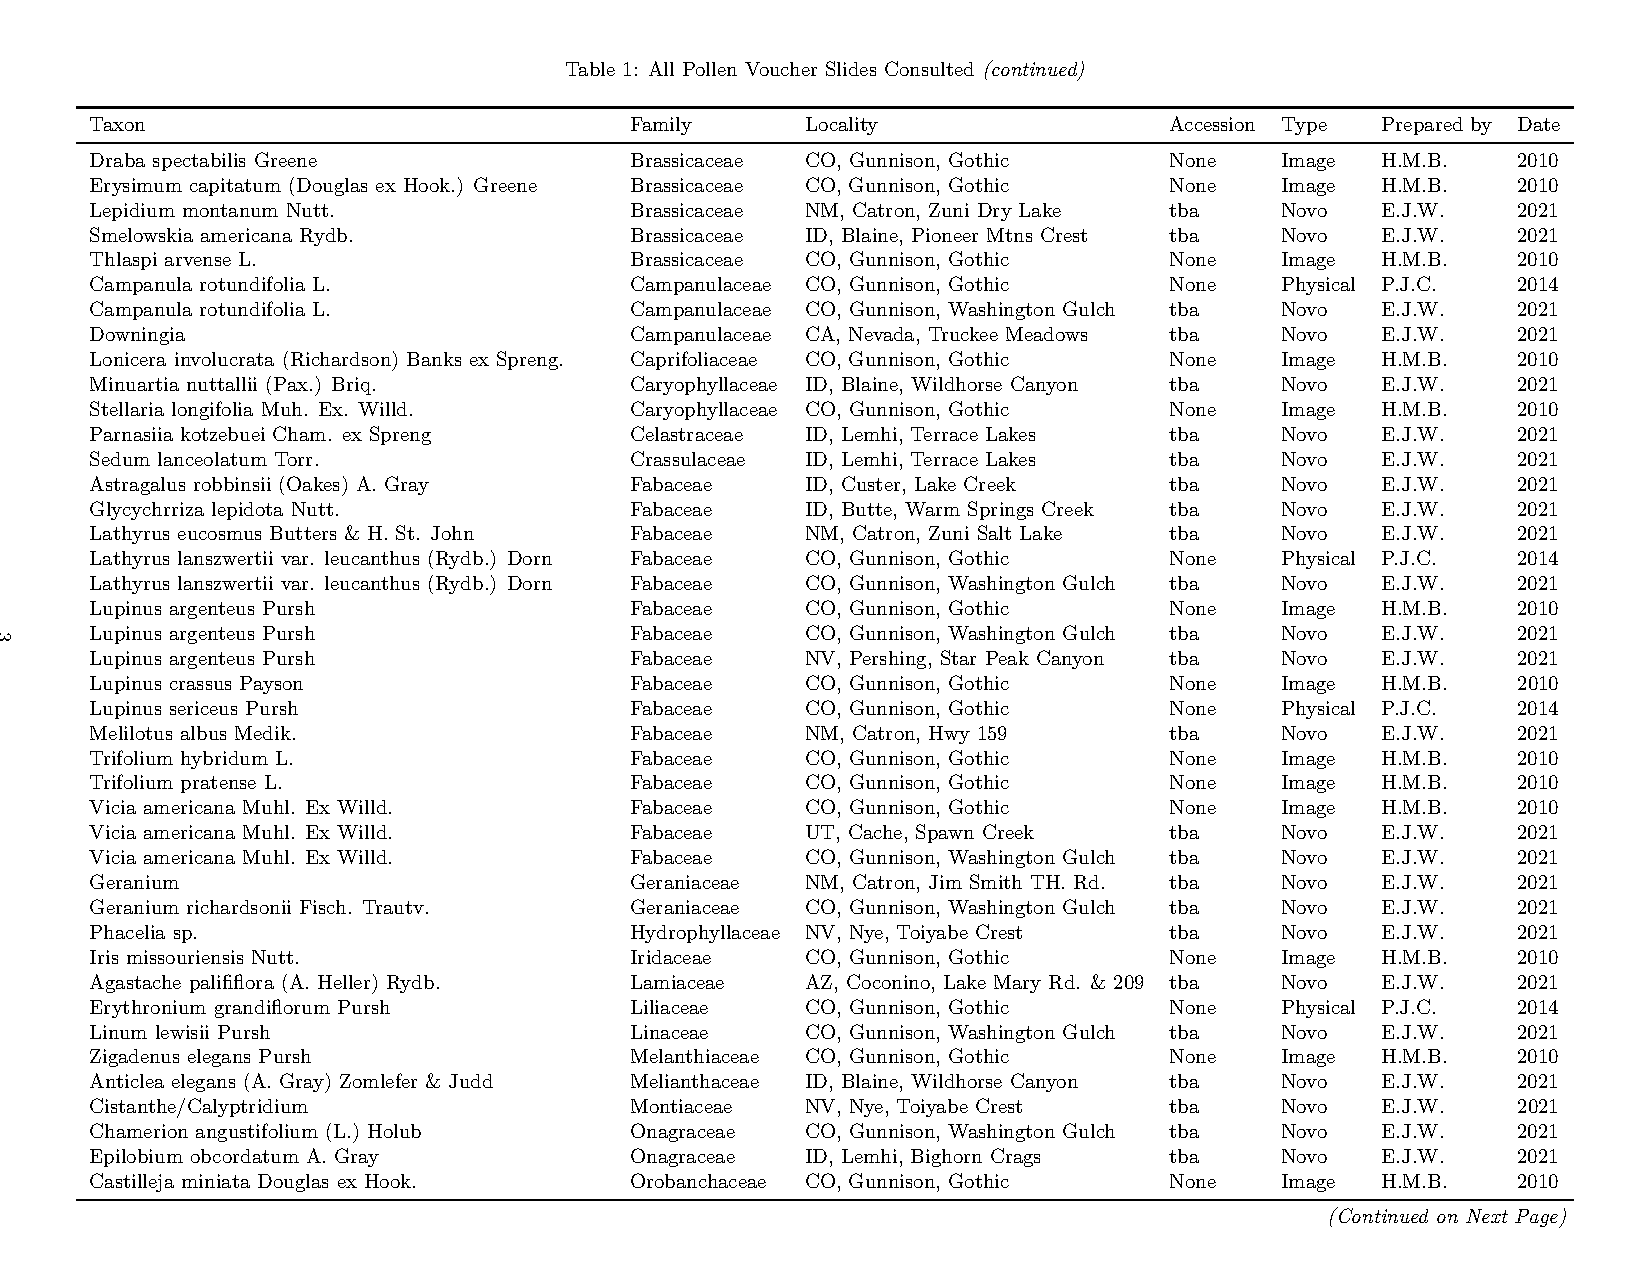
\includegraphics{../graphics/assorted/pollen_slide_table_reduced-2.pdf}

\newpage

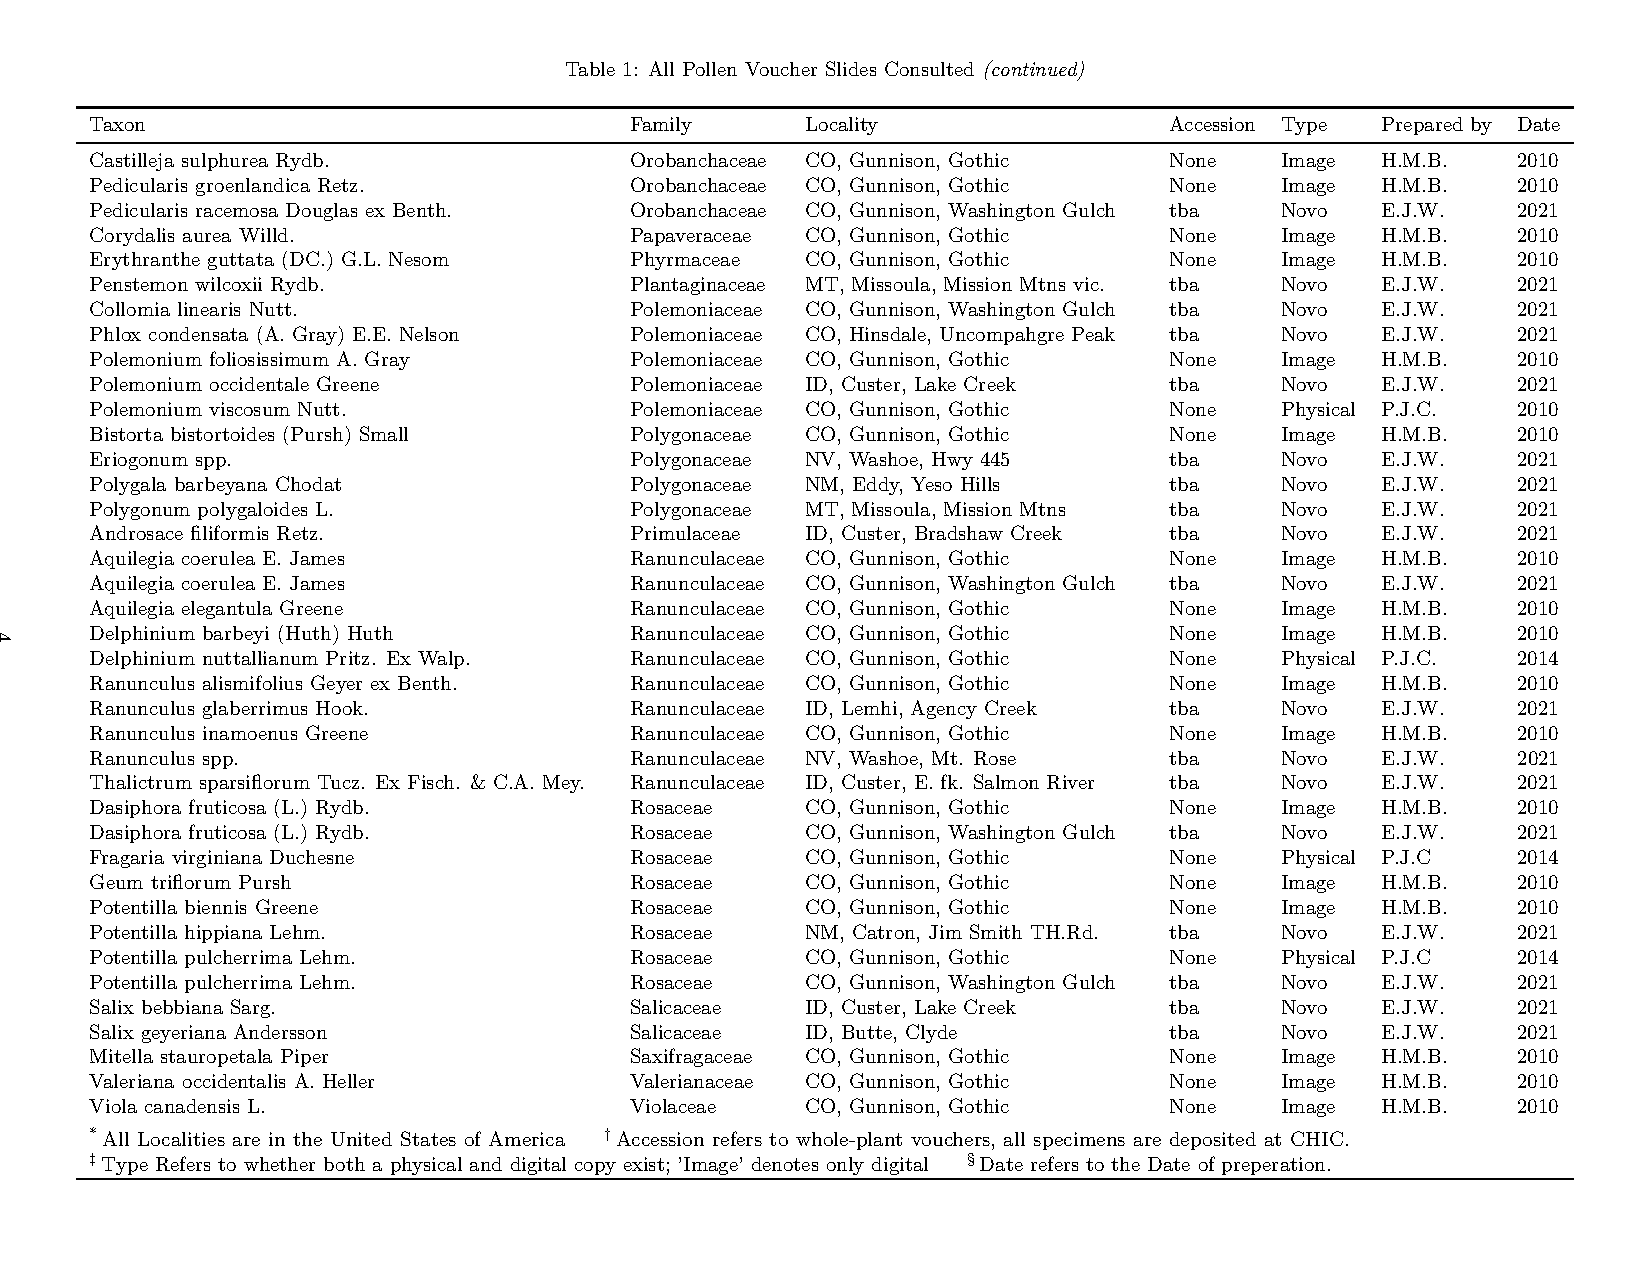
\includegraphics{../graphics/assorted/pollen_slide_table_reduced-3.pdf}

\newpage

\hypertarget{pollen-cluster-results-should-be-here}{%
\subsubsection{POLLEN CLUSTER RESULTS SHOULD BE
HERE}\label{pollen-cluster-results-should-be-here}}

\newpage

Appendix XX - Pollen Key

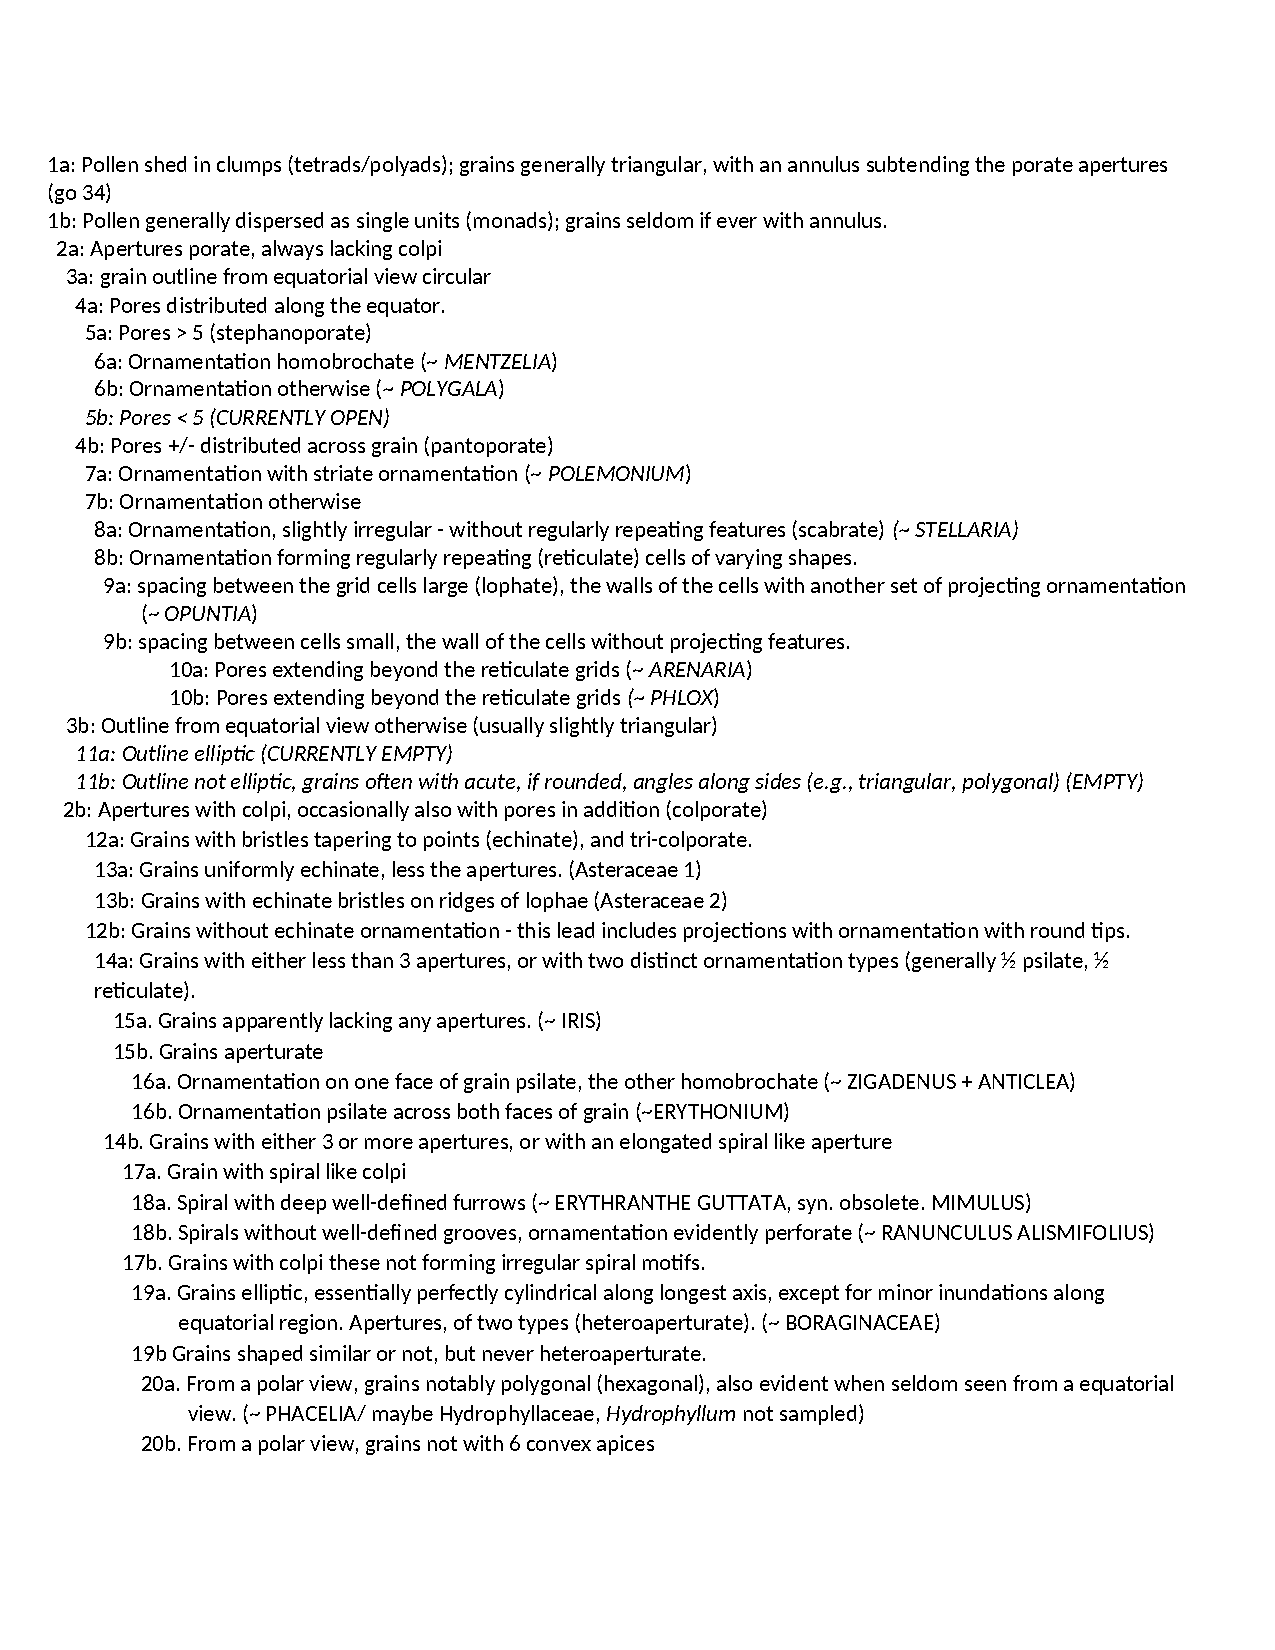
\includegraphics{../graphics/assorted/RMBL_pollen_key-1.pdf}

\newpage

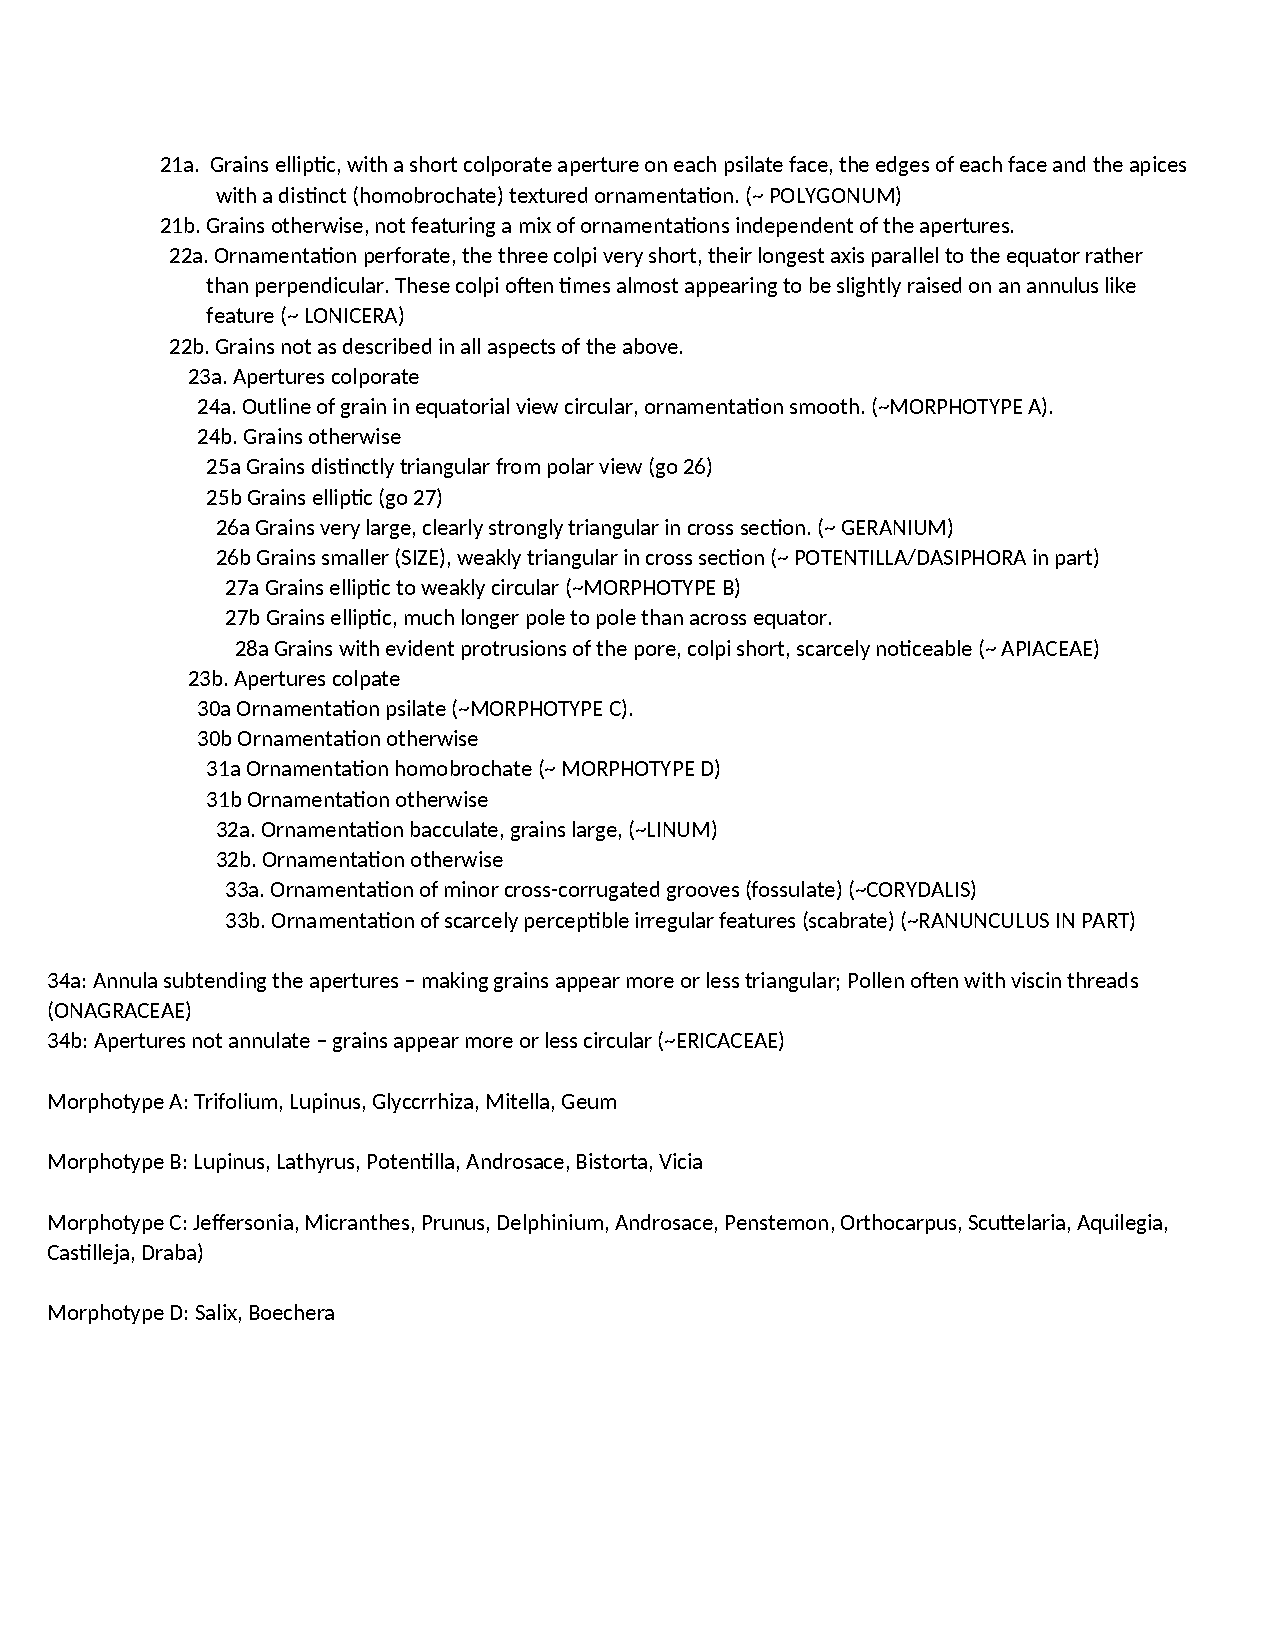
\includegraphics{../graphics/assorted/RMBL_pollen_key-2.pdf}

\newpage

APPENDIX XX - Pollen Morphotype Richness Rarefaction Curves

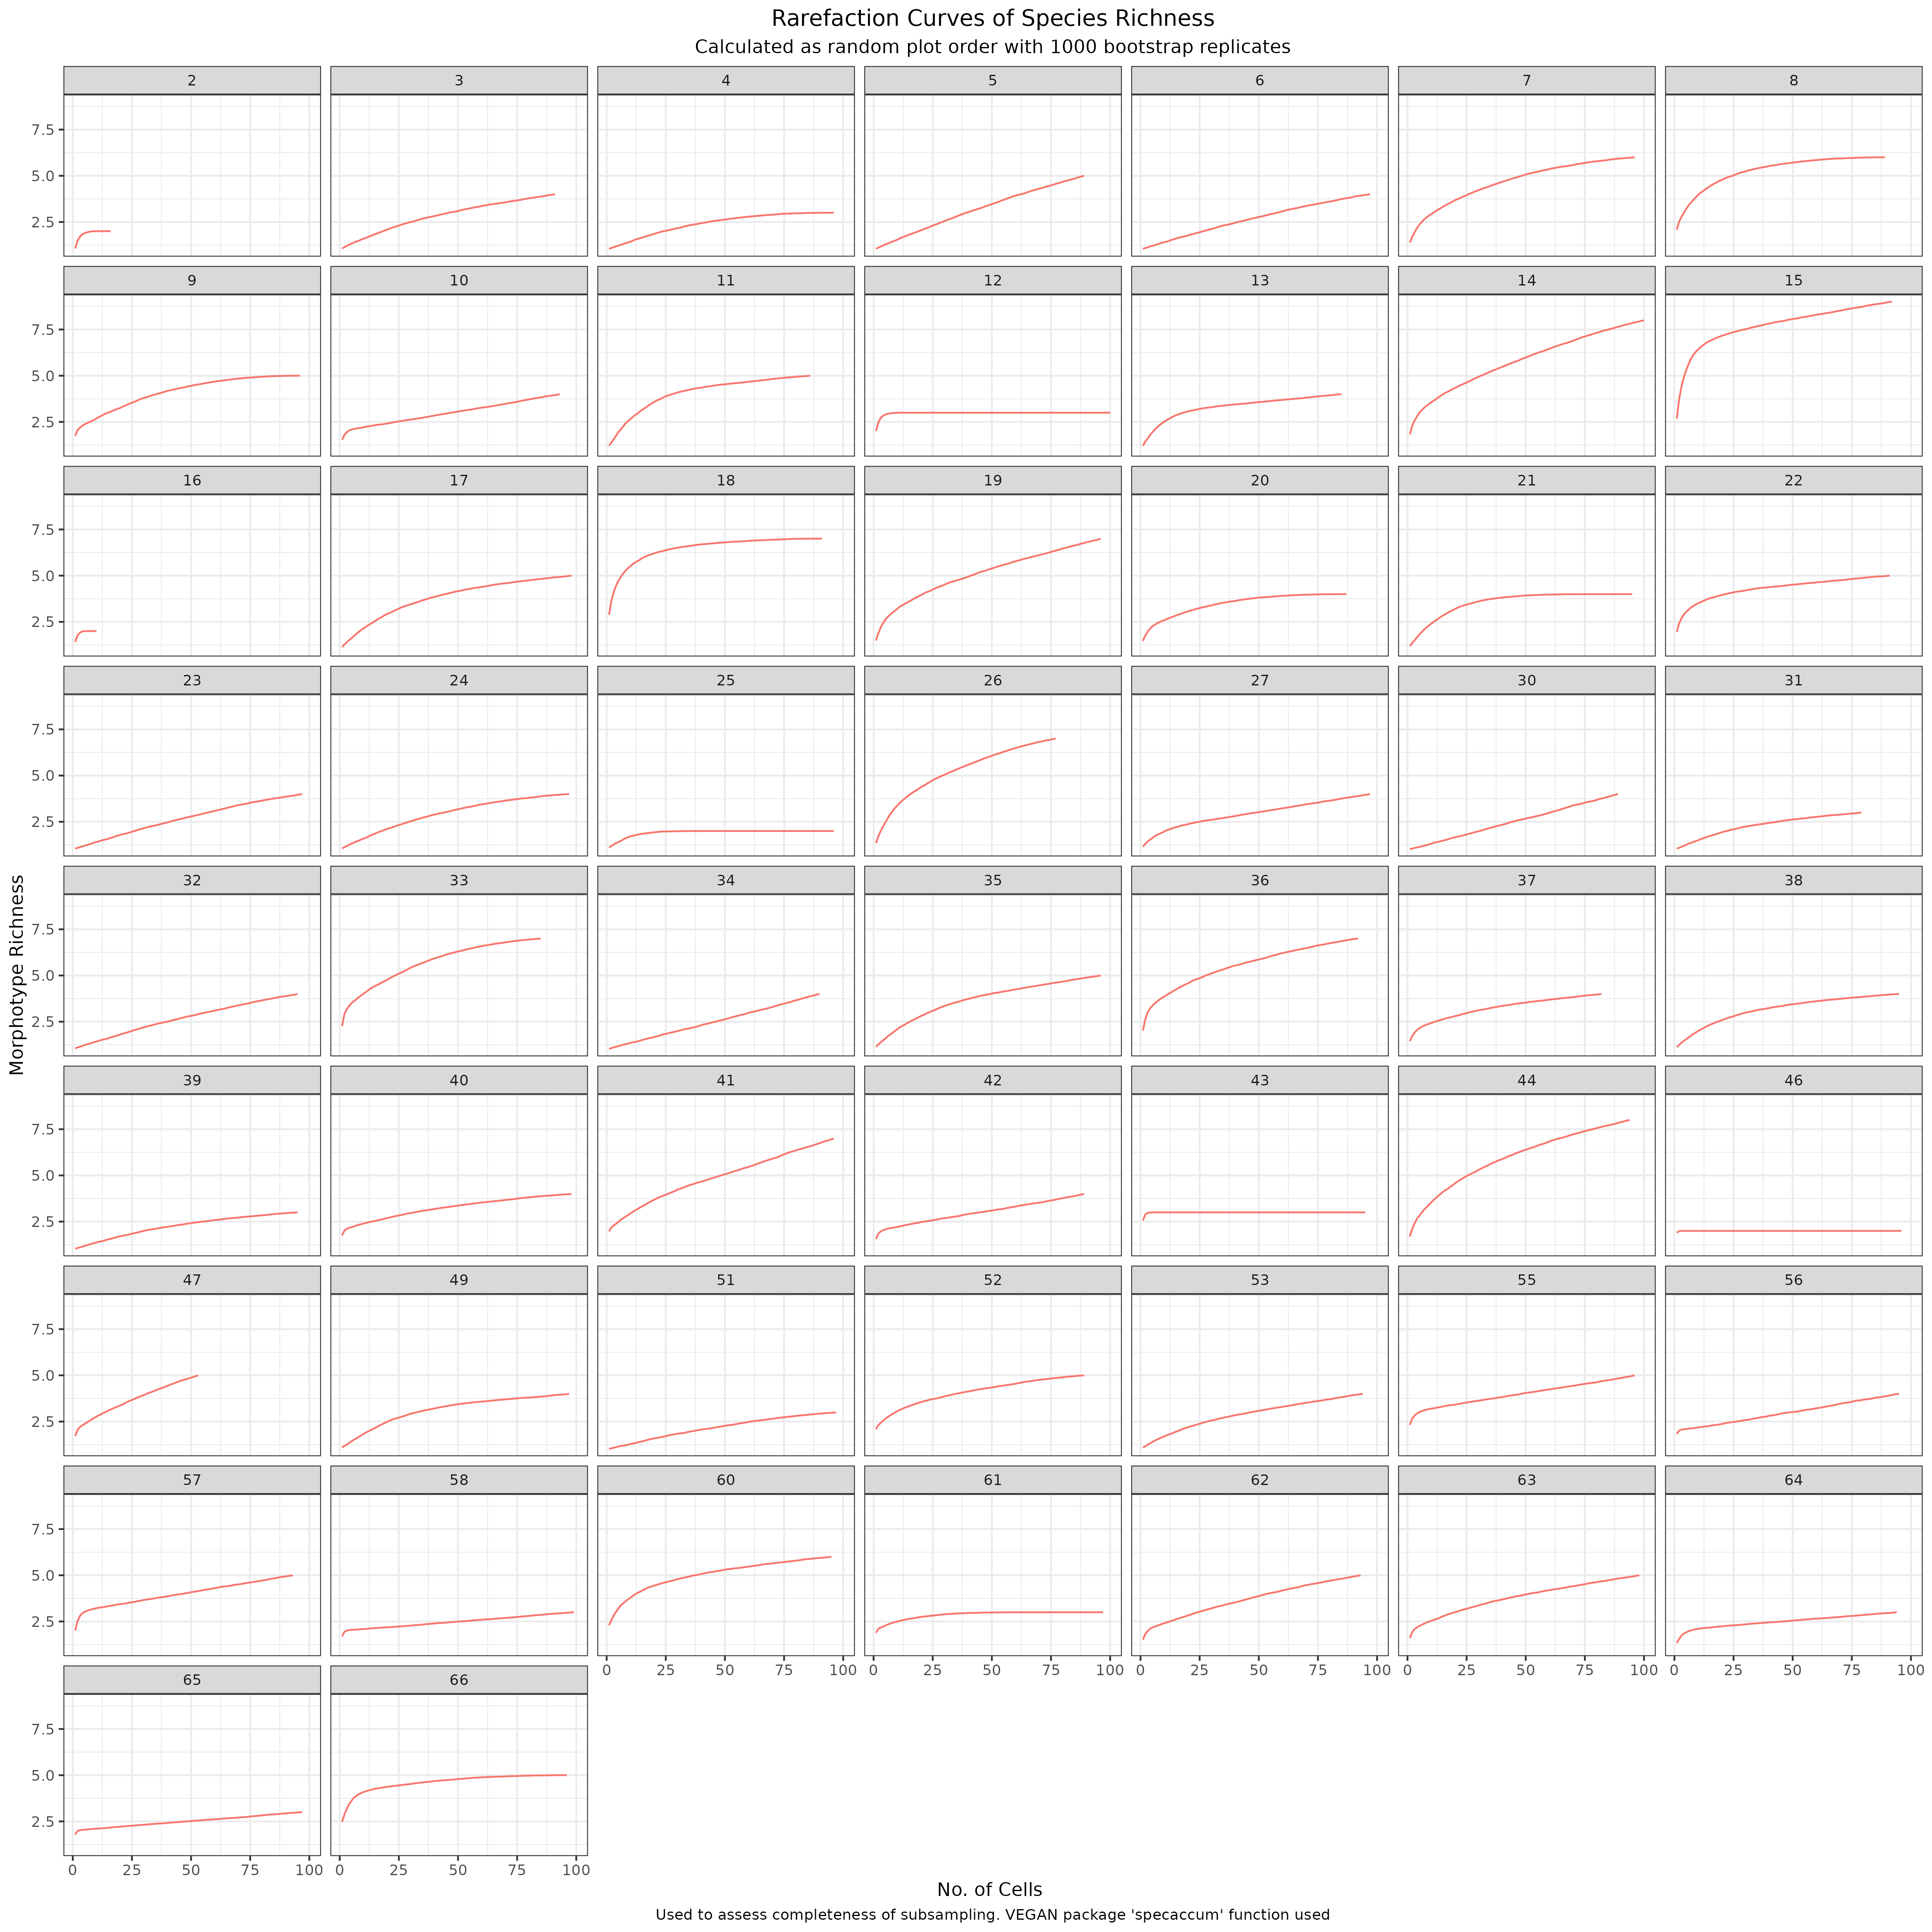
\includegraphics[width=0.95\linewidth]{../graphics/plots/species_richness_rarefaction}

\newpage

Appendix XX - Pollen Morphotype Abundance Rarefaction Curves

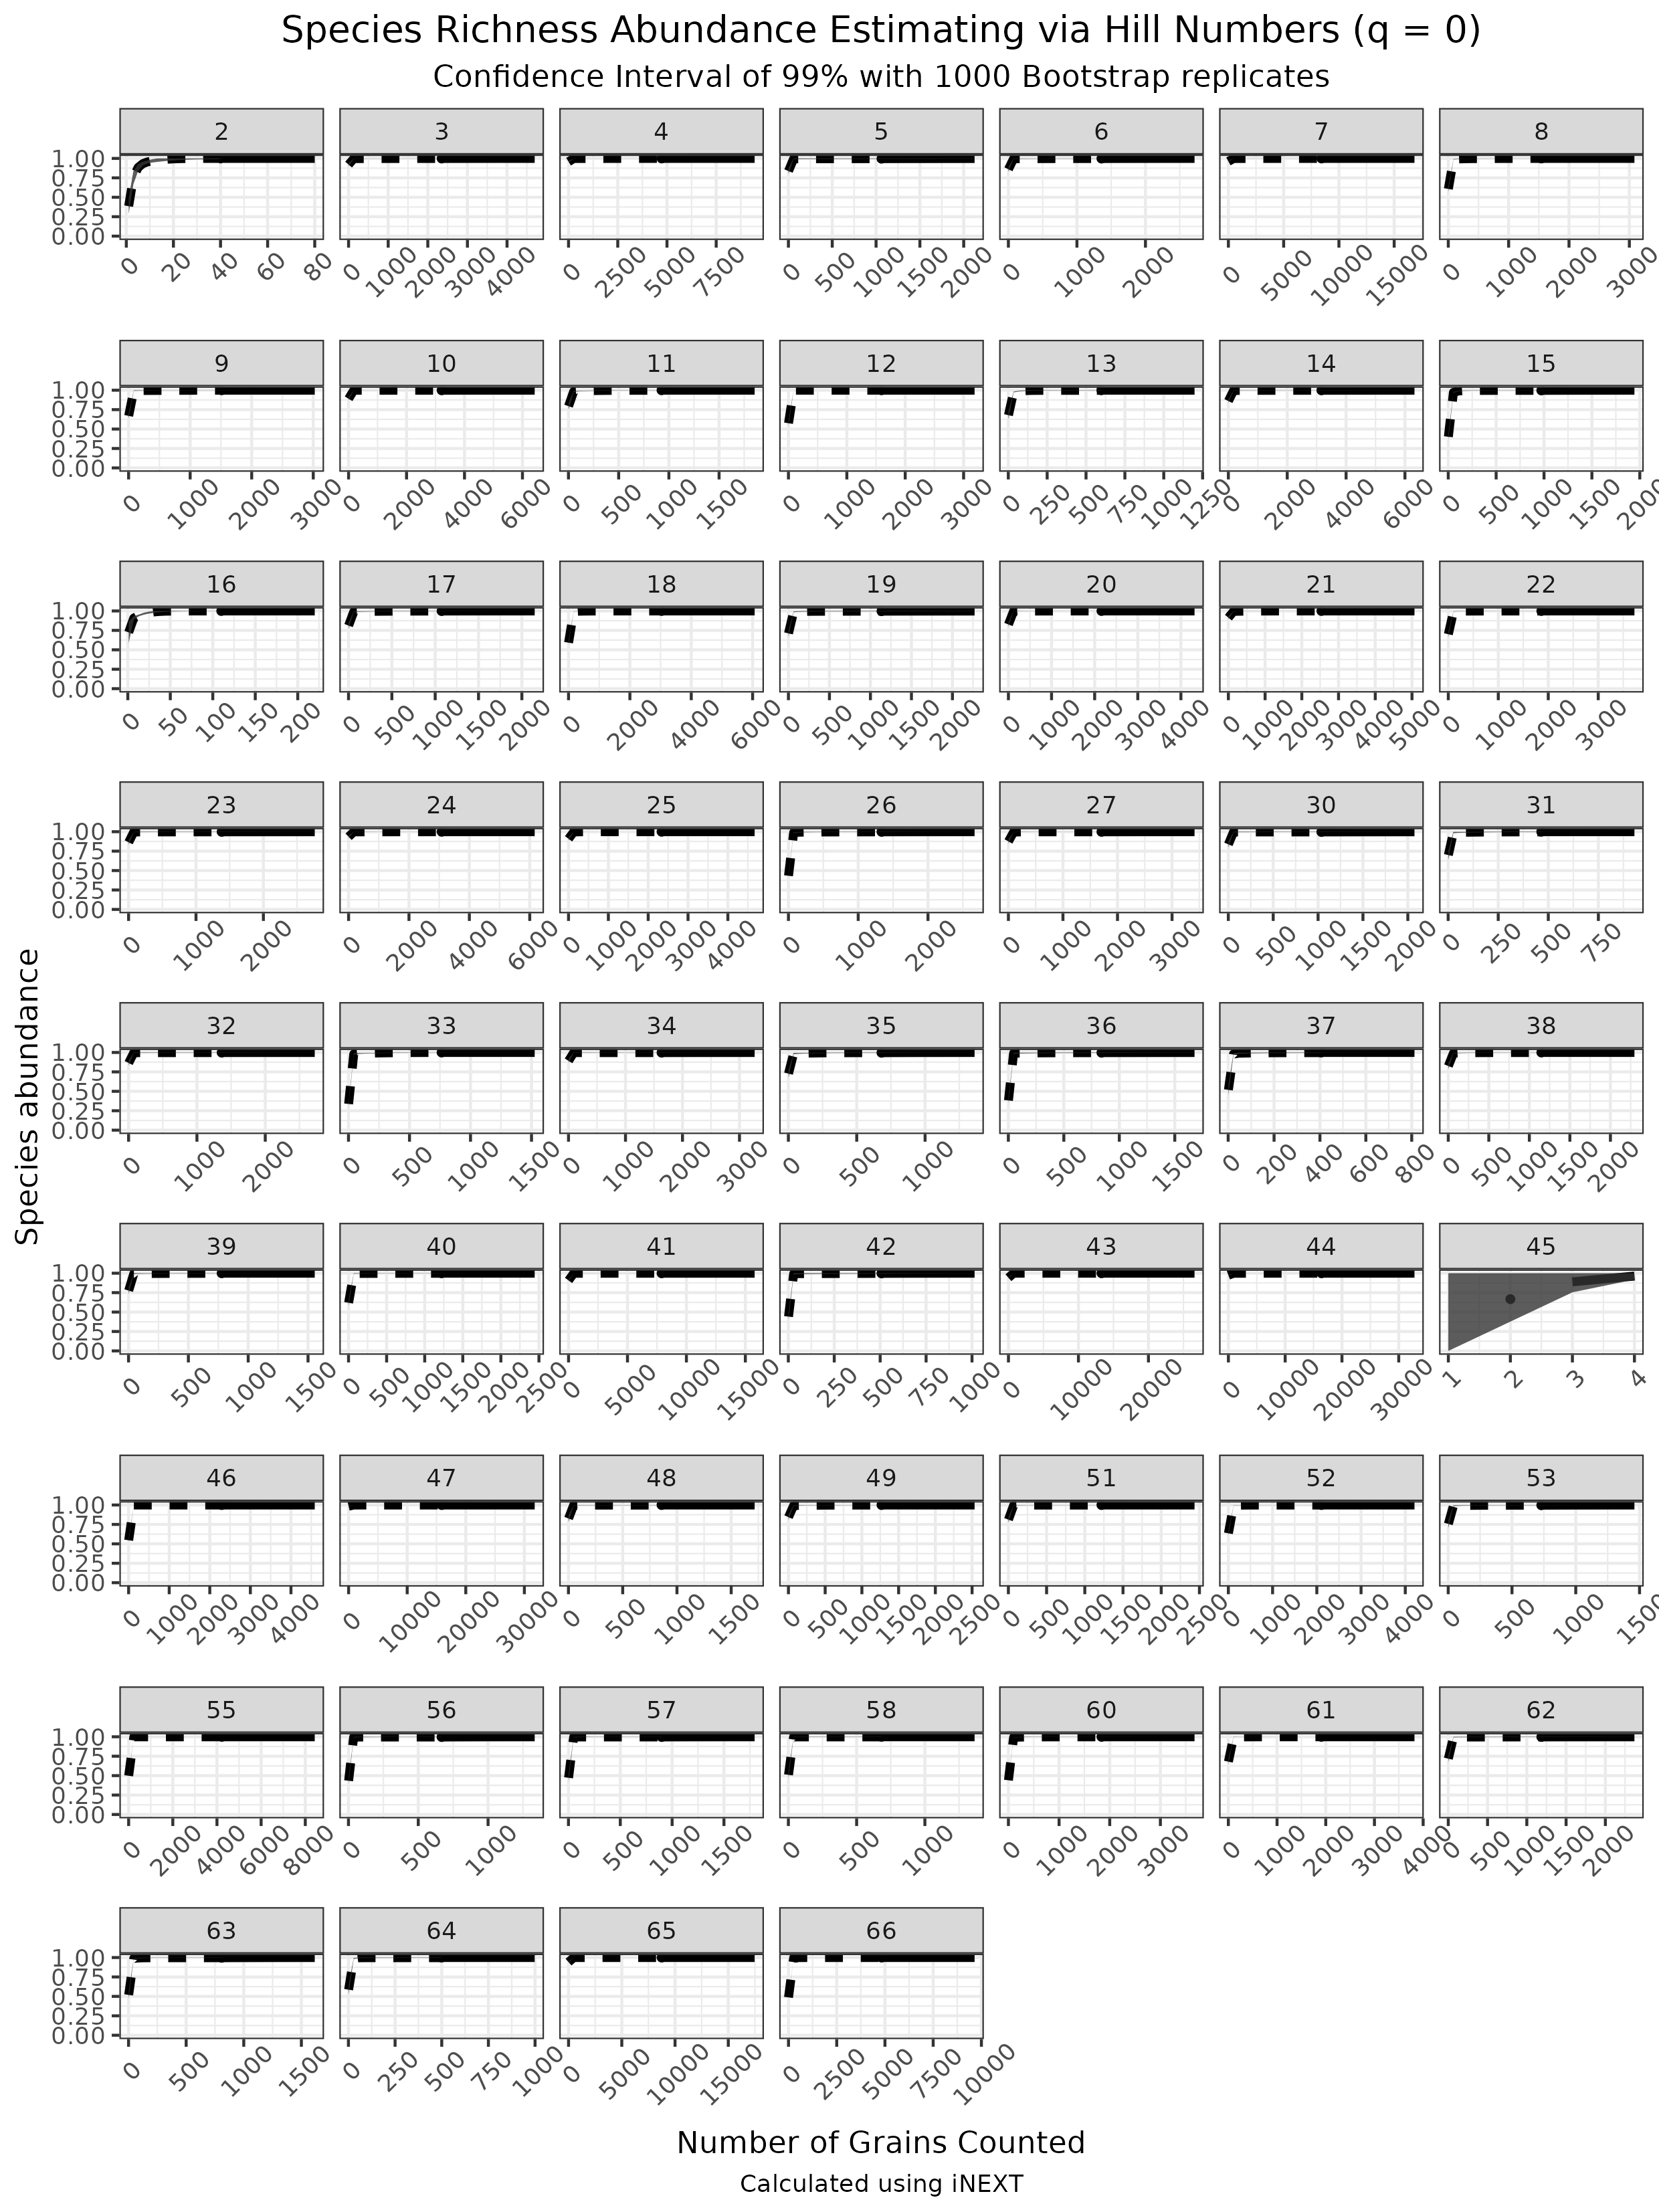
\includegraphics[width=0.99\linewidth]{../graphics/plots/SppAbundance}

\newpage

Appendix XX - All Species in the Sequence Databases

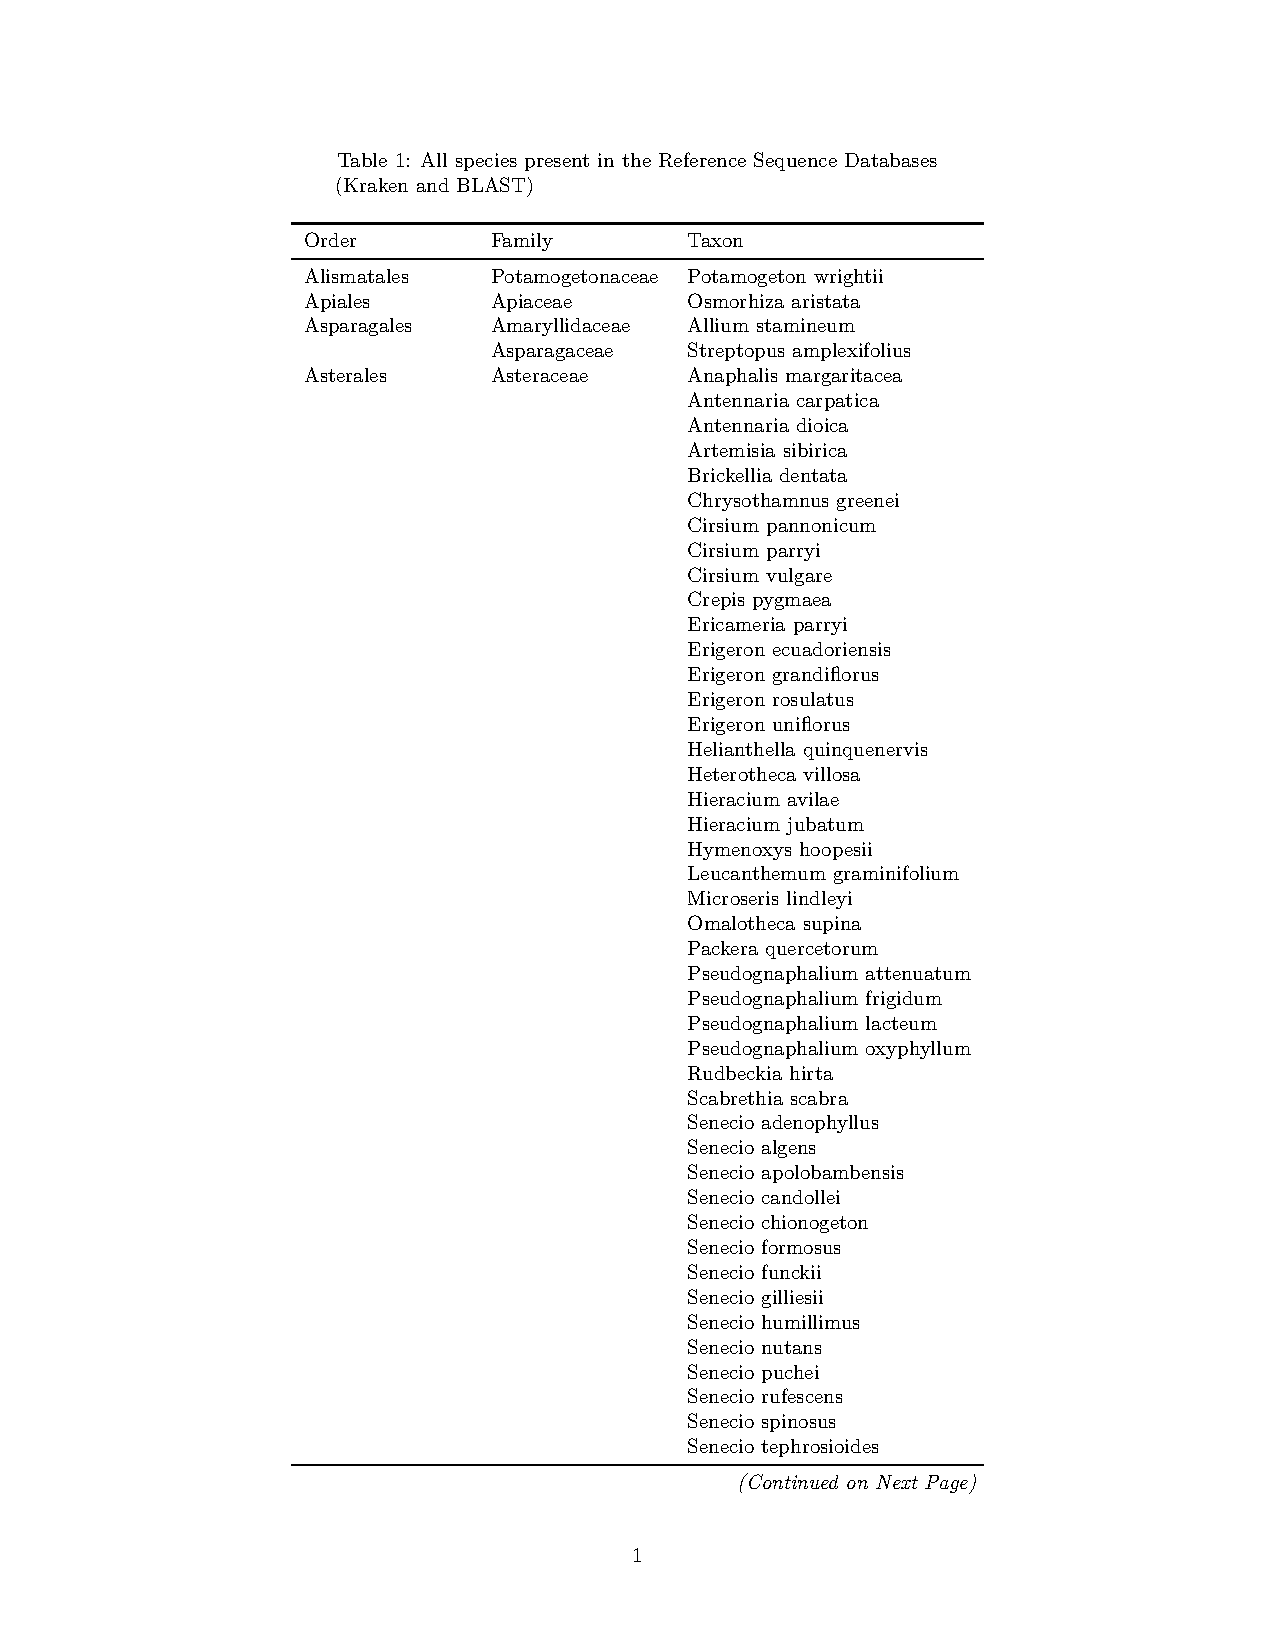
\includegraphics{../graphics/assorted/kraken_db_spp_table-1.pdf}

\newpage

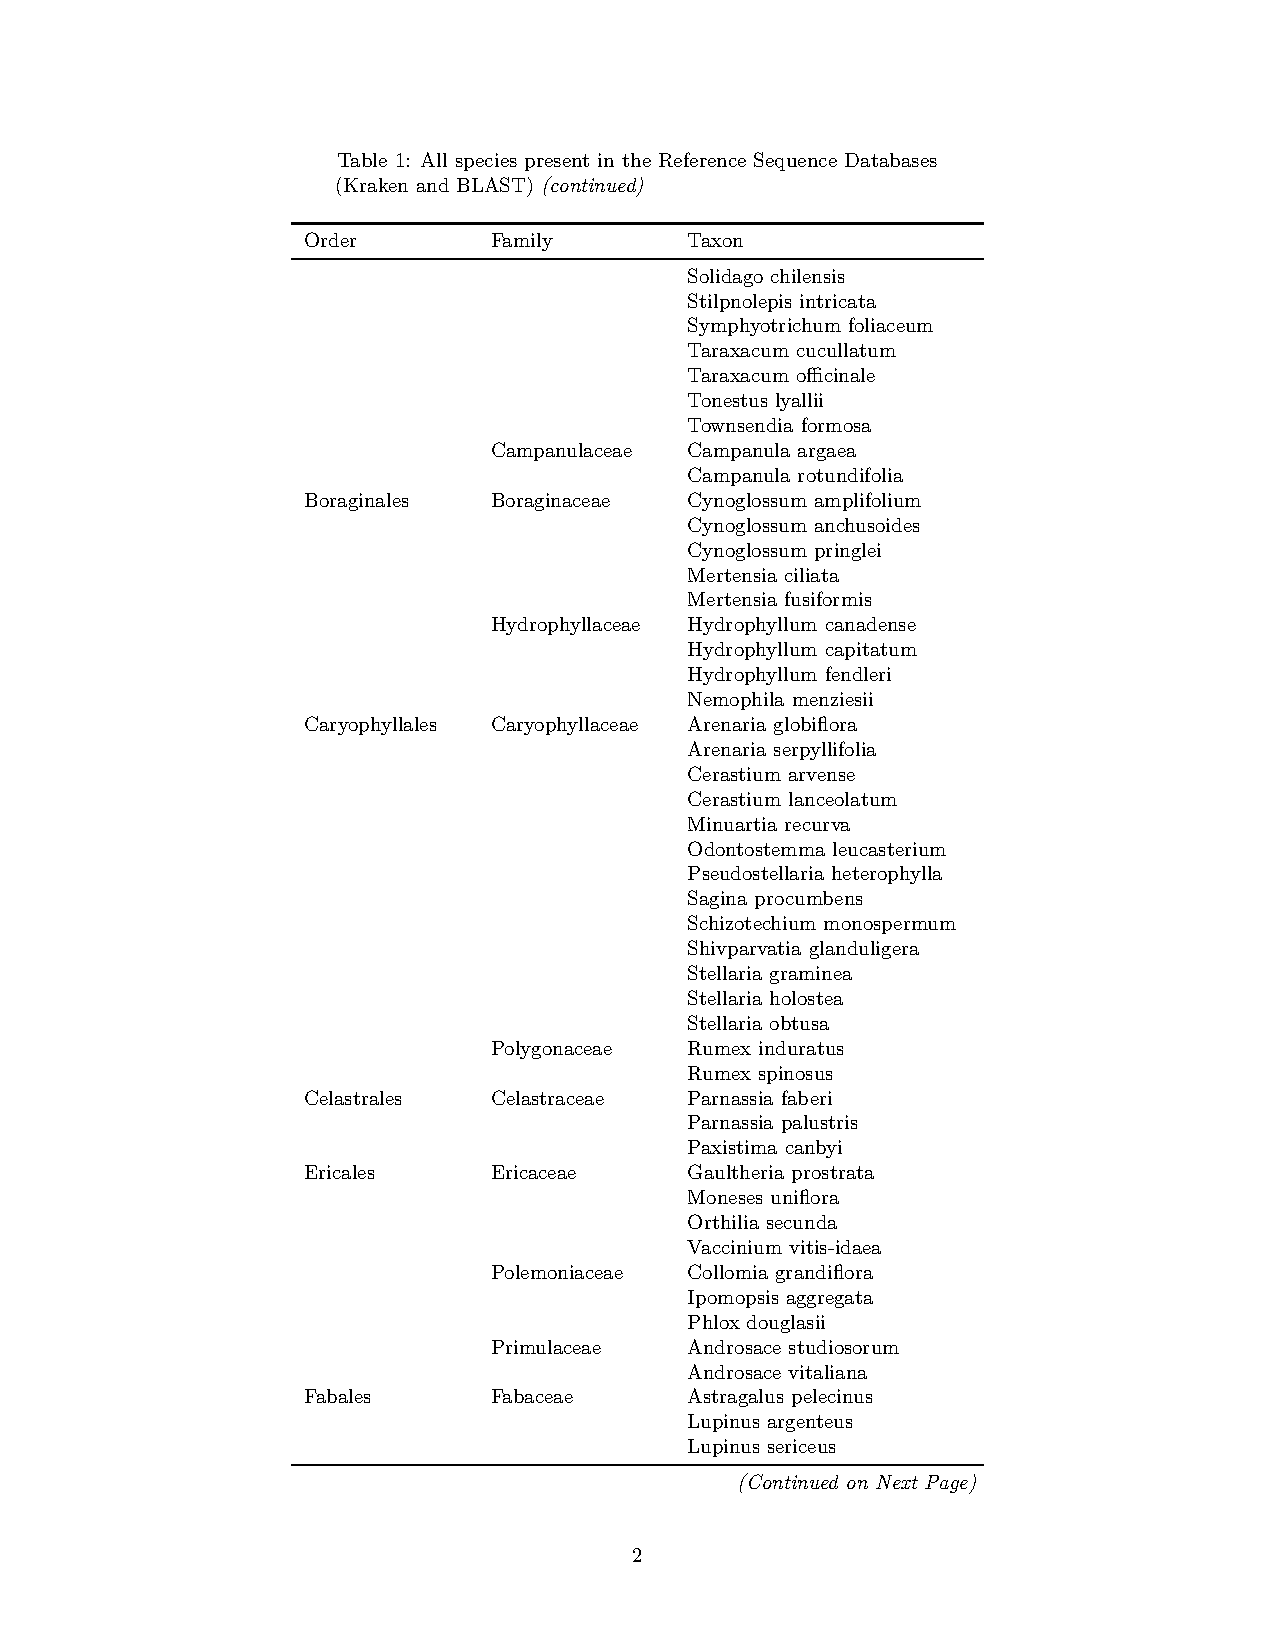
\includegraphics{../graphics/assorted/kraken_db_spp_table-2.pdf}

\newpage

Appendix XX - All Species in the Sequence Databases (con't)

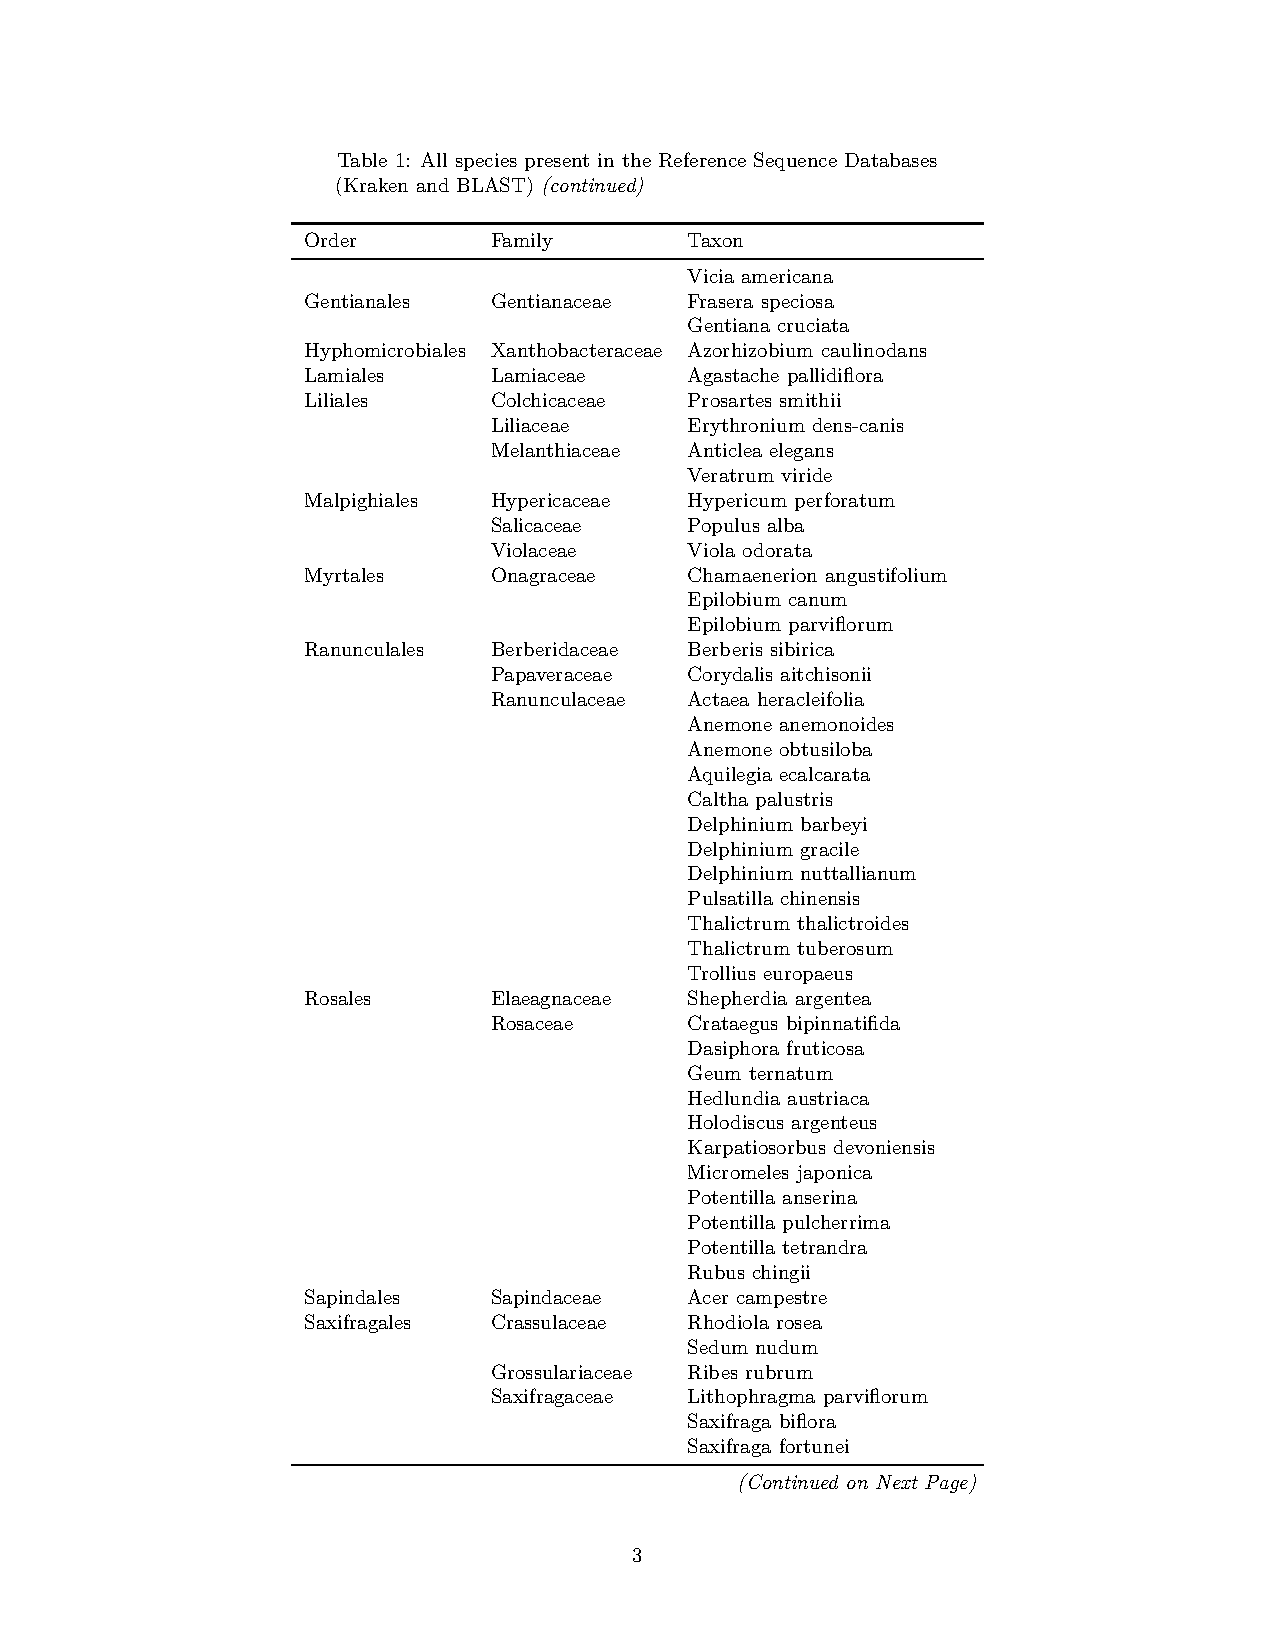
\includegraphics{../graphics/assorted/kraken_db_spp_table-3.pdf}

\newpage

Appendix XX - All Species in the Sequence Databases (con't)


\includegraphics{../graphics/assorted/kraken_db_spp_table-4.pdf}

\newpage

Appendix XX - Reads Per Loci

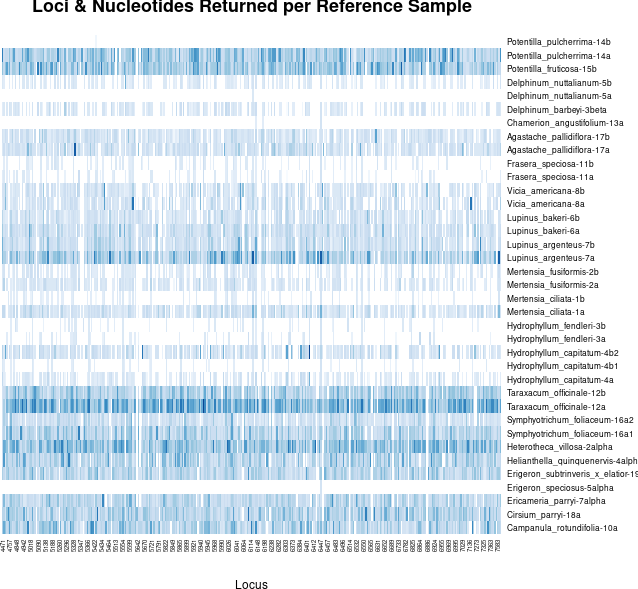
\includegraphics[width=0.98\linewidth]{../graphics/plots/Loci_Reference_Samples}

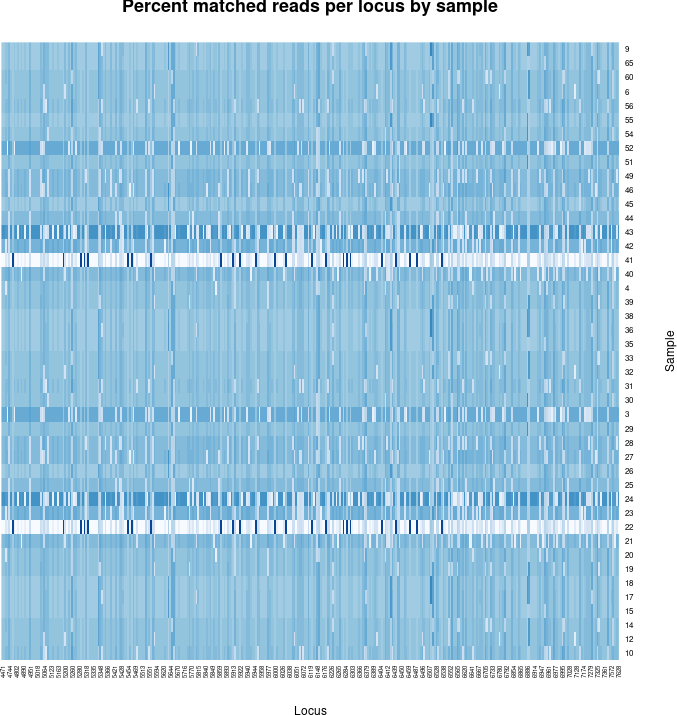
\includegraphics[width=0.98\linewidth]{../graphics/plots/Percent_loci_matched_by_sample}

\newpage

Appendix XX - Comparison of Kraken2, Bracken, and BLAST

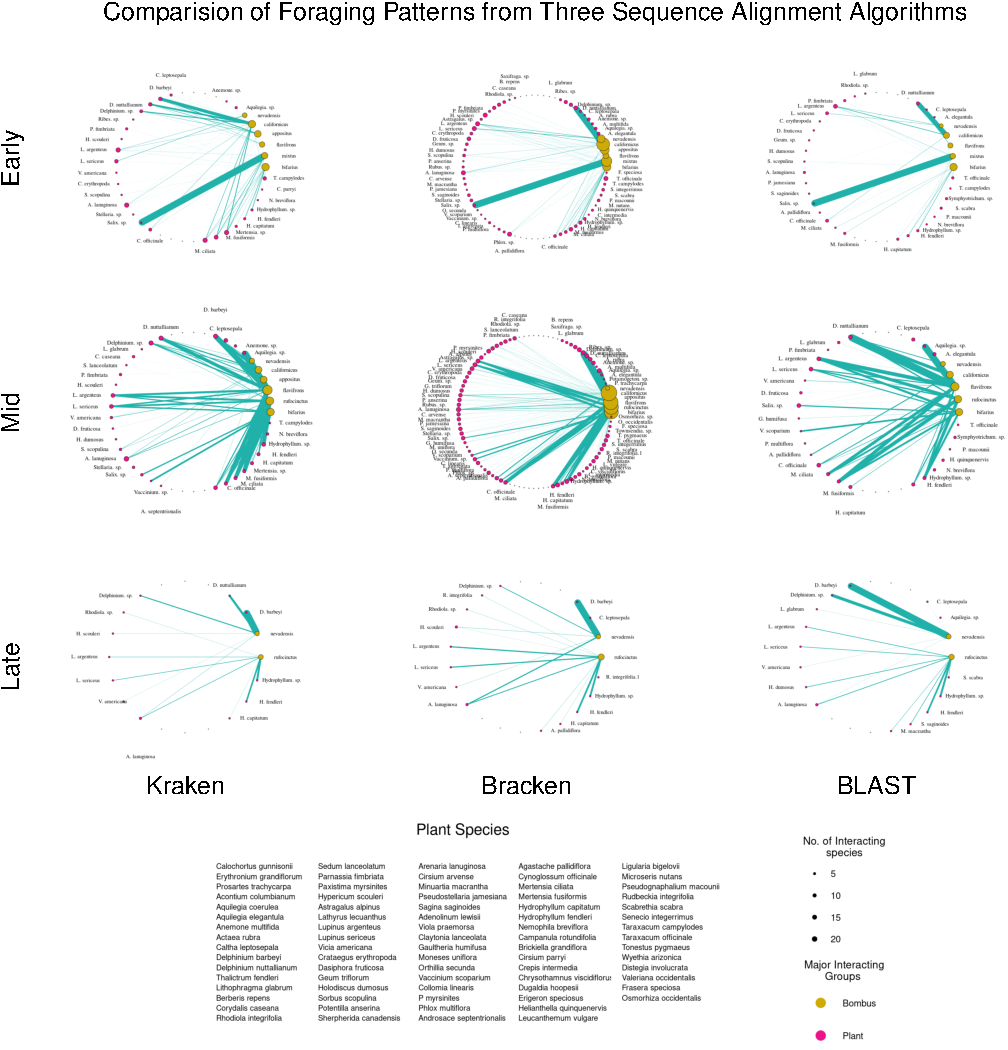
\includegraphics[width=1.1\linewidth]{../graphics/plots/Molecular_nets-crop}

\newpage

Appendix XX - Models used for Species Distribution Model Ensembles

The two machine learning models utilize Ensemble learning.

\textbf{Ensemble learning} utilizes many sets of trees, each tree being
composed of many binary decisions, to create a single model. Each
independent variable ( - or \emph{feature}) may become a node on the
tree - i.e.~a location on the tree where a binary decision will move
towards a predicted outcome. Each of the decision tree models which
ensemble learning utilizes is a weak model, each of which may suffer due
to high variance or bias, but which produce better outcomes than would
be expected via chance. When ensembled these models generate a strong
model, a model which should have more appropriately balanced variance
and bias and predicts outcomes which are more strongly correlated with
the expected values than the individual weak models.

\emph{\textbf{Random Forest (RF)}} the training data are continually
bootstrap re-sampled, in combination with random subsets of features, to
create nodes which attempt to optimally predict a known outcome. A large
number of trees are then aggregated, via the most common predictions, to
generate a final classification prediction tree. Each individual
prediction tree is generated independently of the others.

\emph{\textbf{Boosted Regression Tree (BRT)}} (or Gradient Boosted tree)
An initial tree is grown, and all other trees are derived sequentially
from it, as each new tree is grown the errors in responses from the last
tree are weighed more heavily so that the model focuses on selecting
dependent variables which refine predictions. All response data and
predictor variables are kept available to all trees.

\emph{\textbf{Bias}} predictions from an algorithm are systematically in
error due to being prejudiced for or against certain results, due to
assumptions during learning.

\emph{\textbf{Variance}} errors in models due to an over-reliance and
sensitivity of training to outliers in training data.

In general, Random Forest models have high bias and low variance, where
boosted regressions trees have lower bias and higher variance.
Theoretically, the weaknesses and strengths of bootstrap aggregation
(bagging) as implemented by Random Forests are supplemented by the
boosting.

\newpage

APPENDIX XX - Time Spent Generating Species Distribution Models

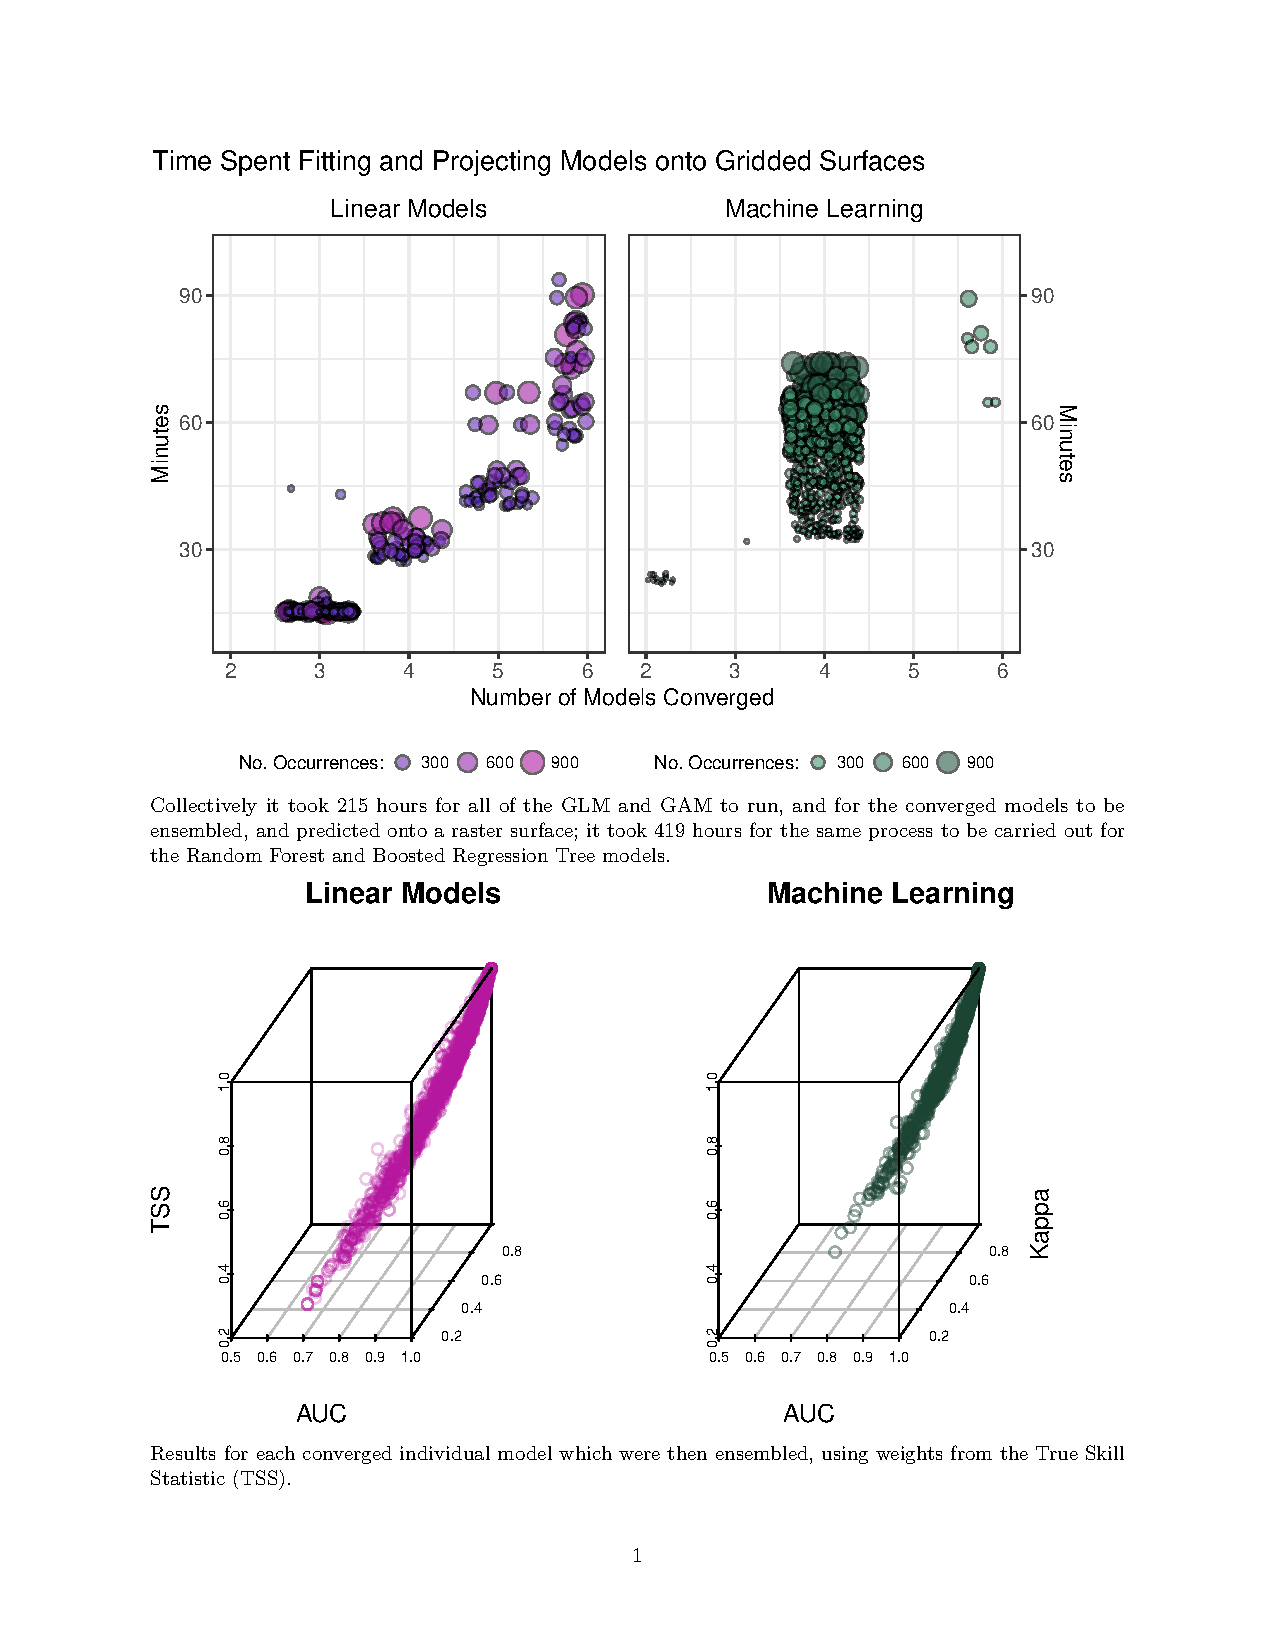
\includegraphics{../graphics/assorted/individual_model_runs.pdf}

\newpage

APPENDIX XX - Review Classified Reads and Reassign

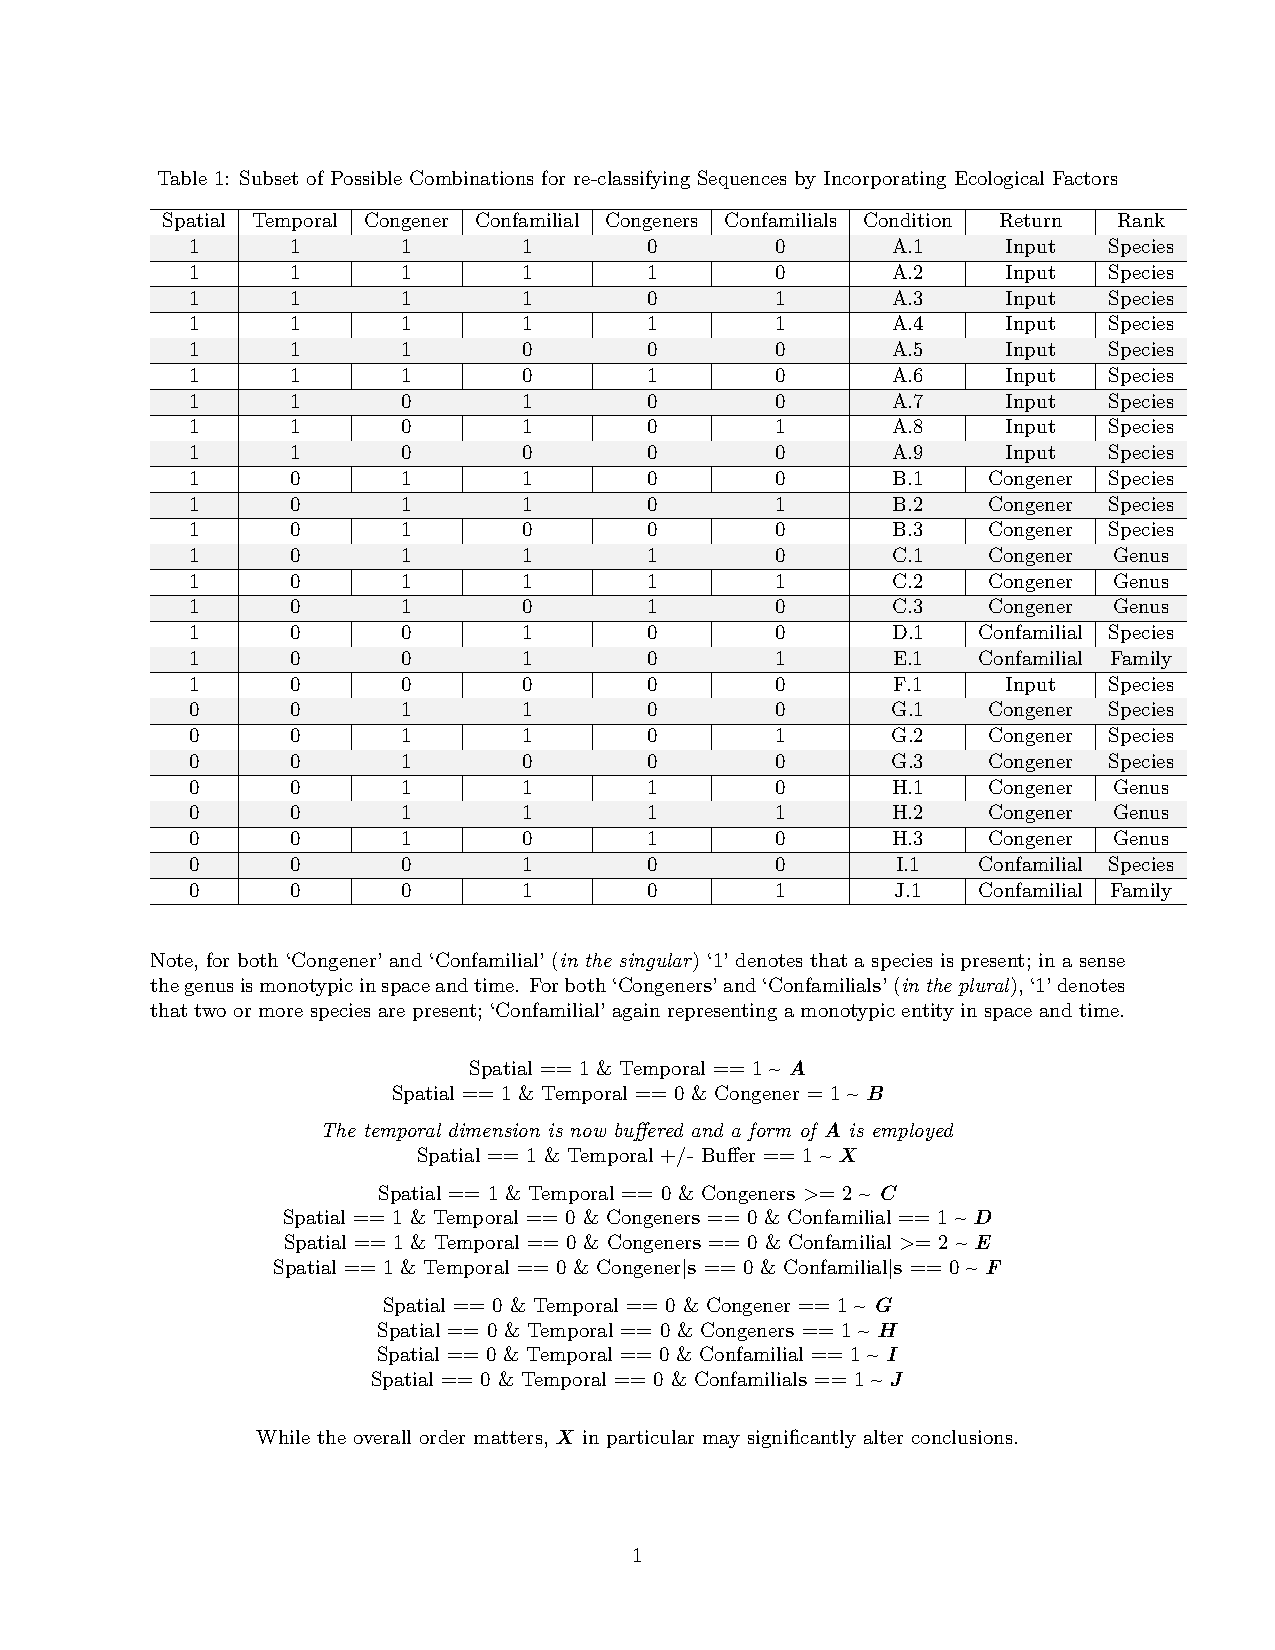
\includegraphics{../graphics/tables/reclassify_reads_table.pdf}

\newpage

APPENDIX XX - Tips and tricks for implementing plant metagenomic
sequencing

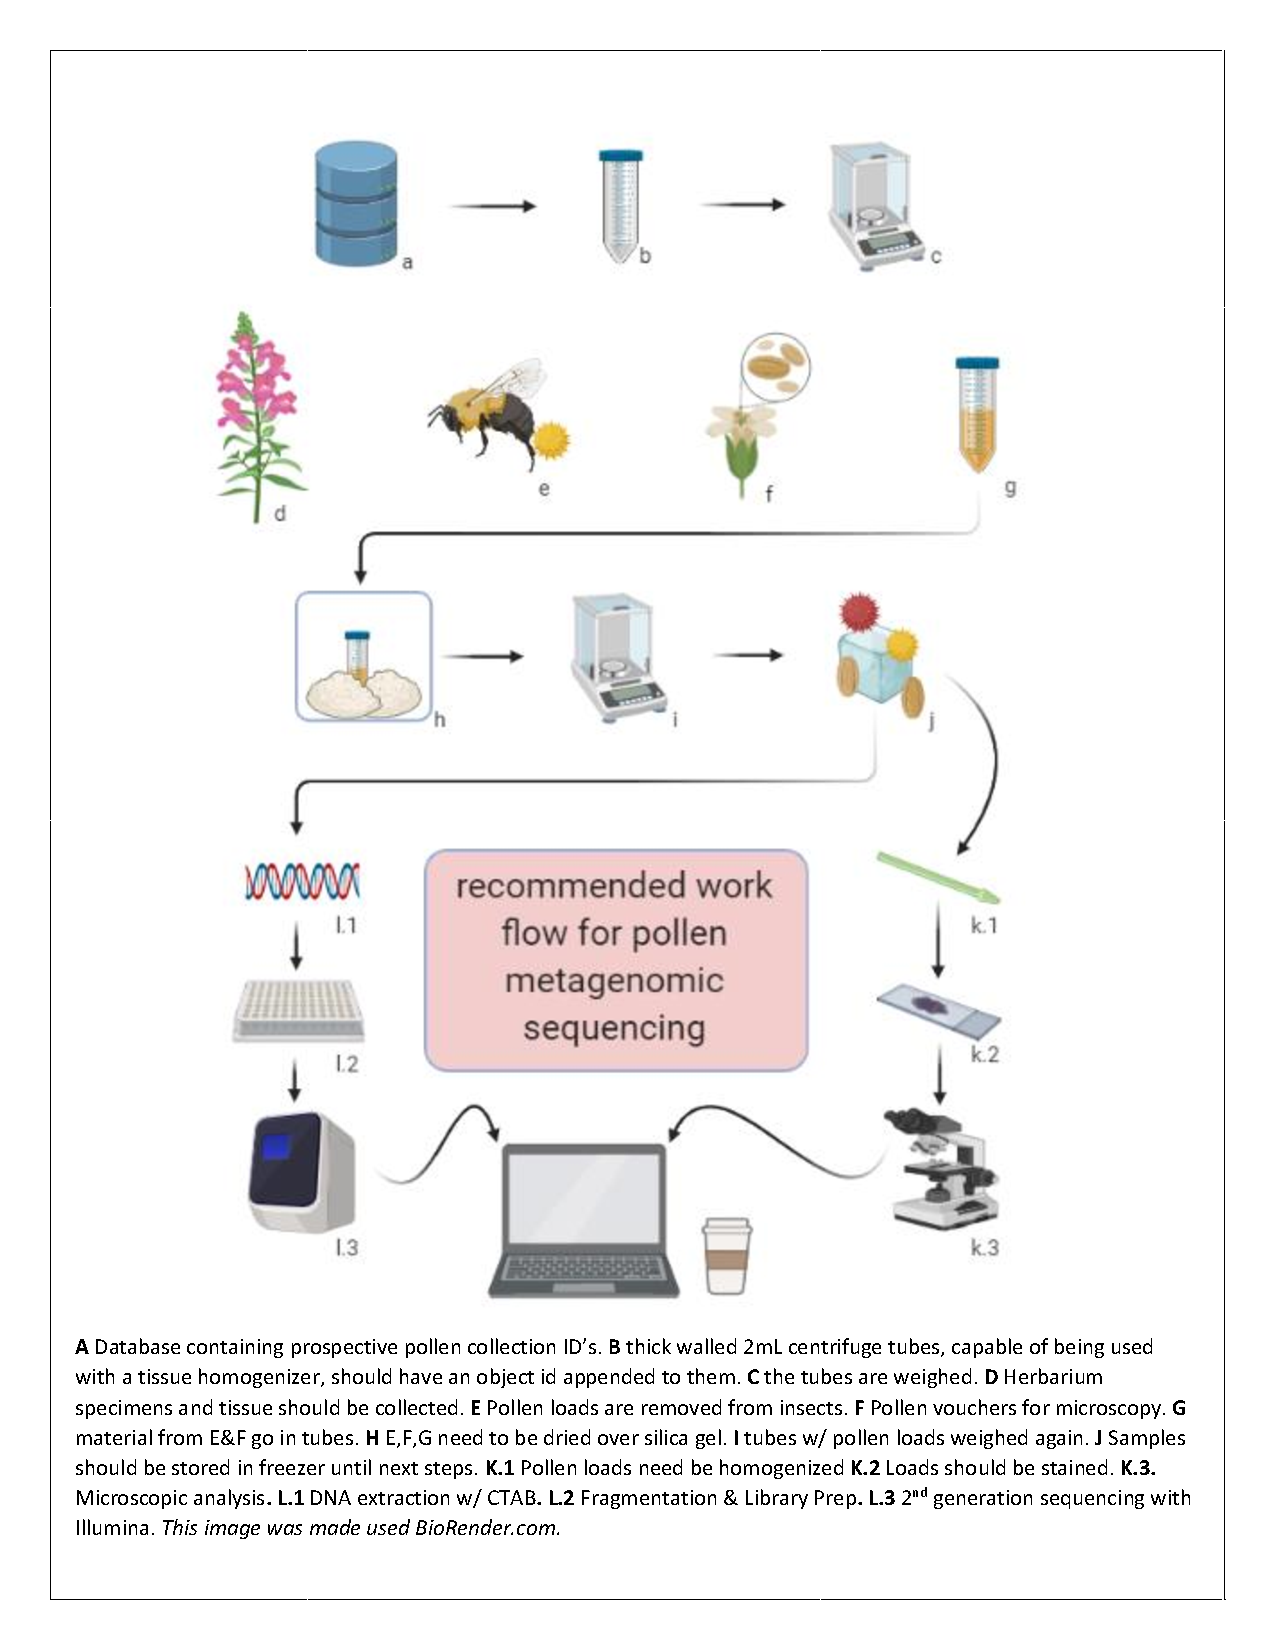
\includegraphics{../graphics/assorted/overall_metagenomic_workflow.pdf}

\newpage

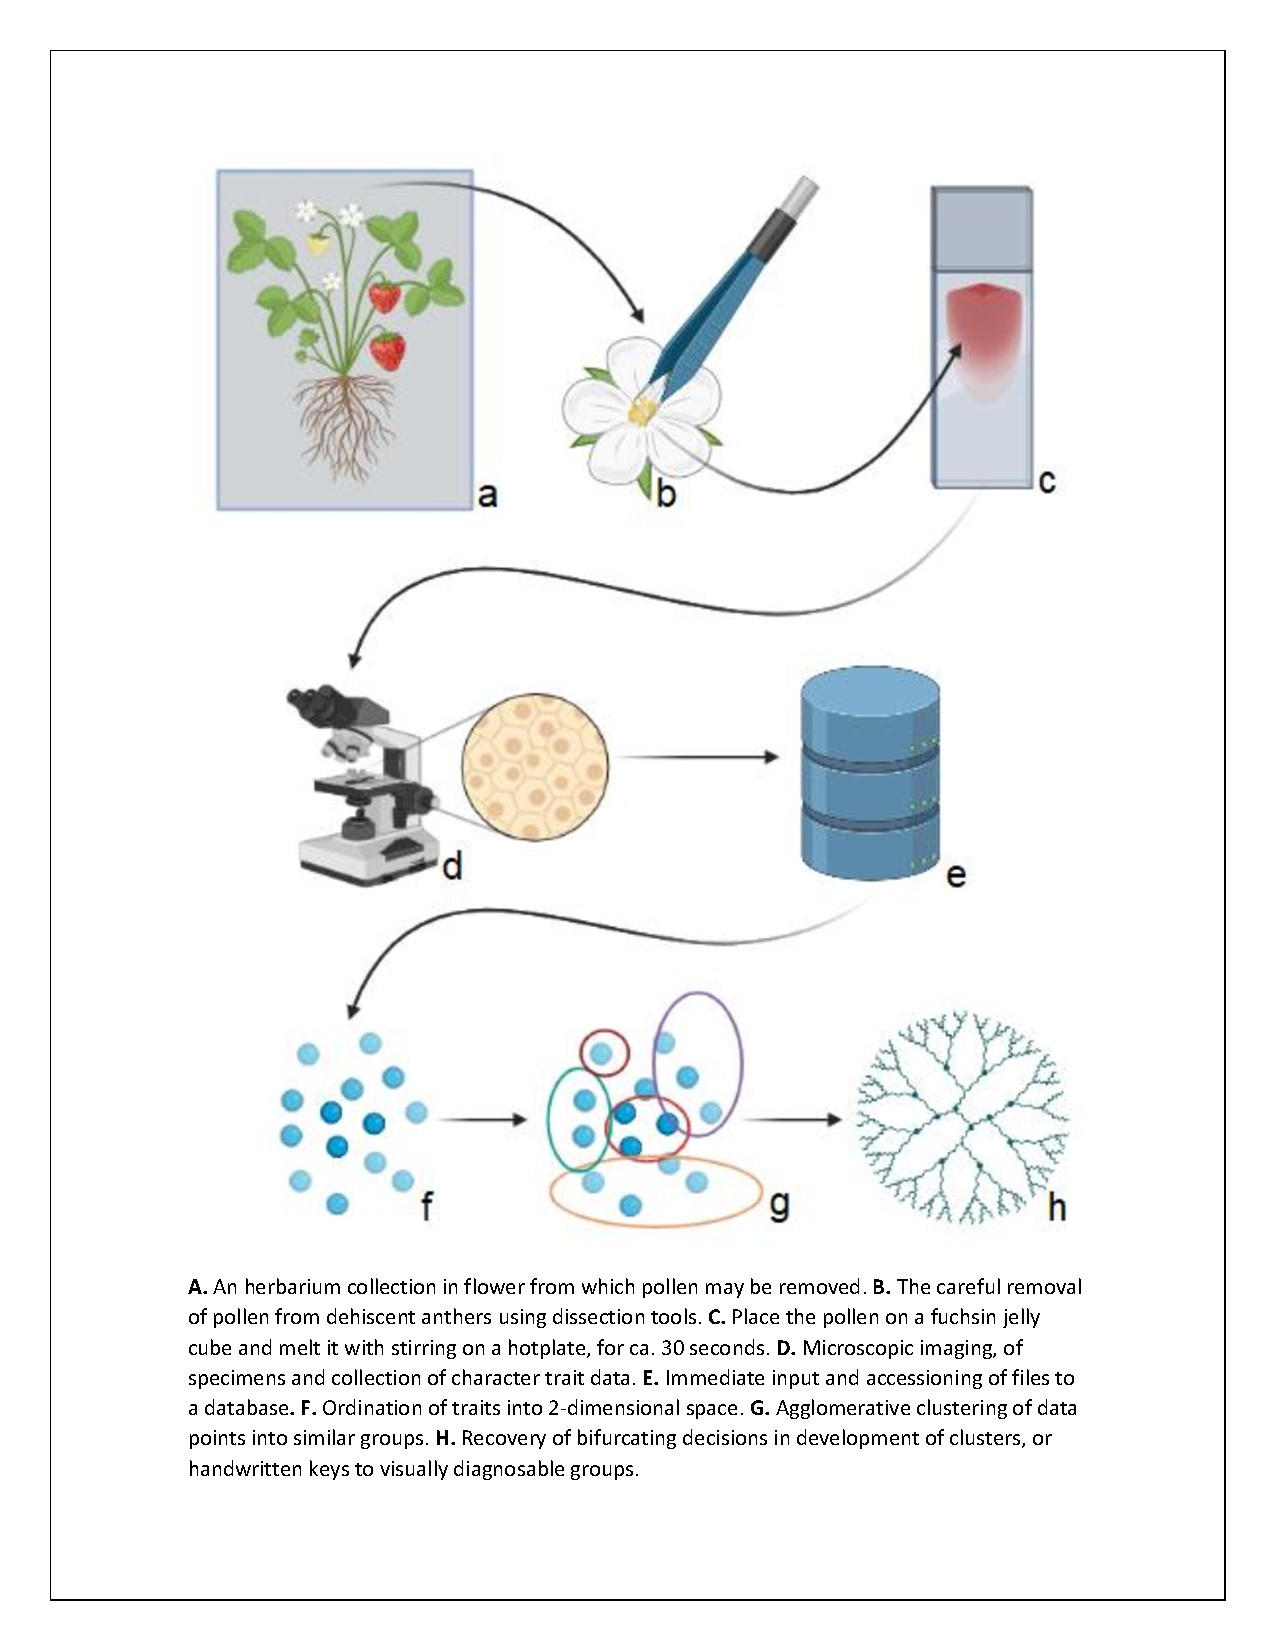
\includegraphics{../graphics/assorted/microscopy_workflow.pdf}

\newpage

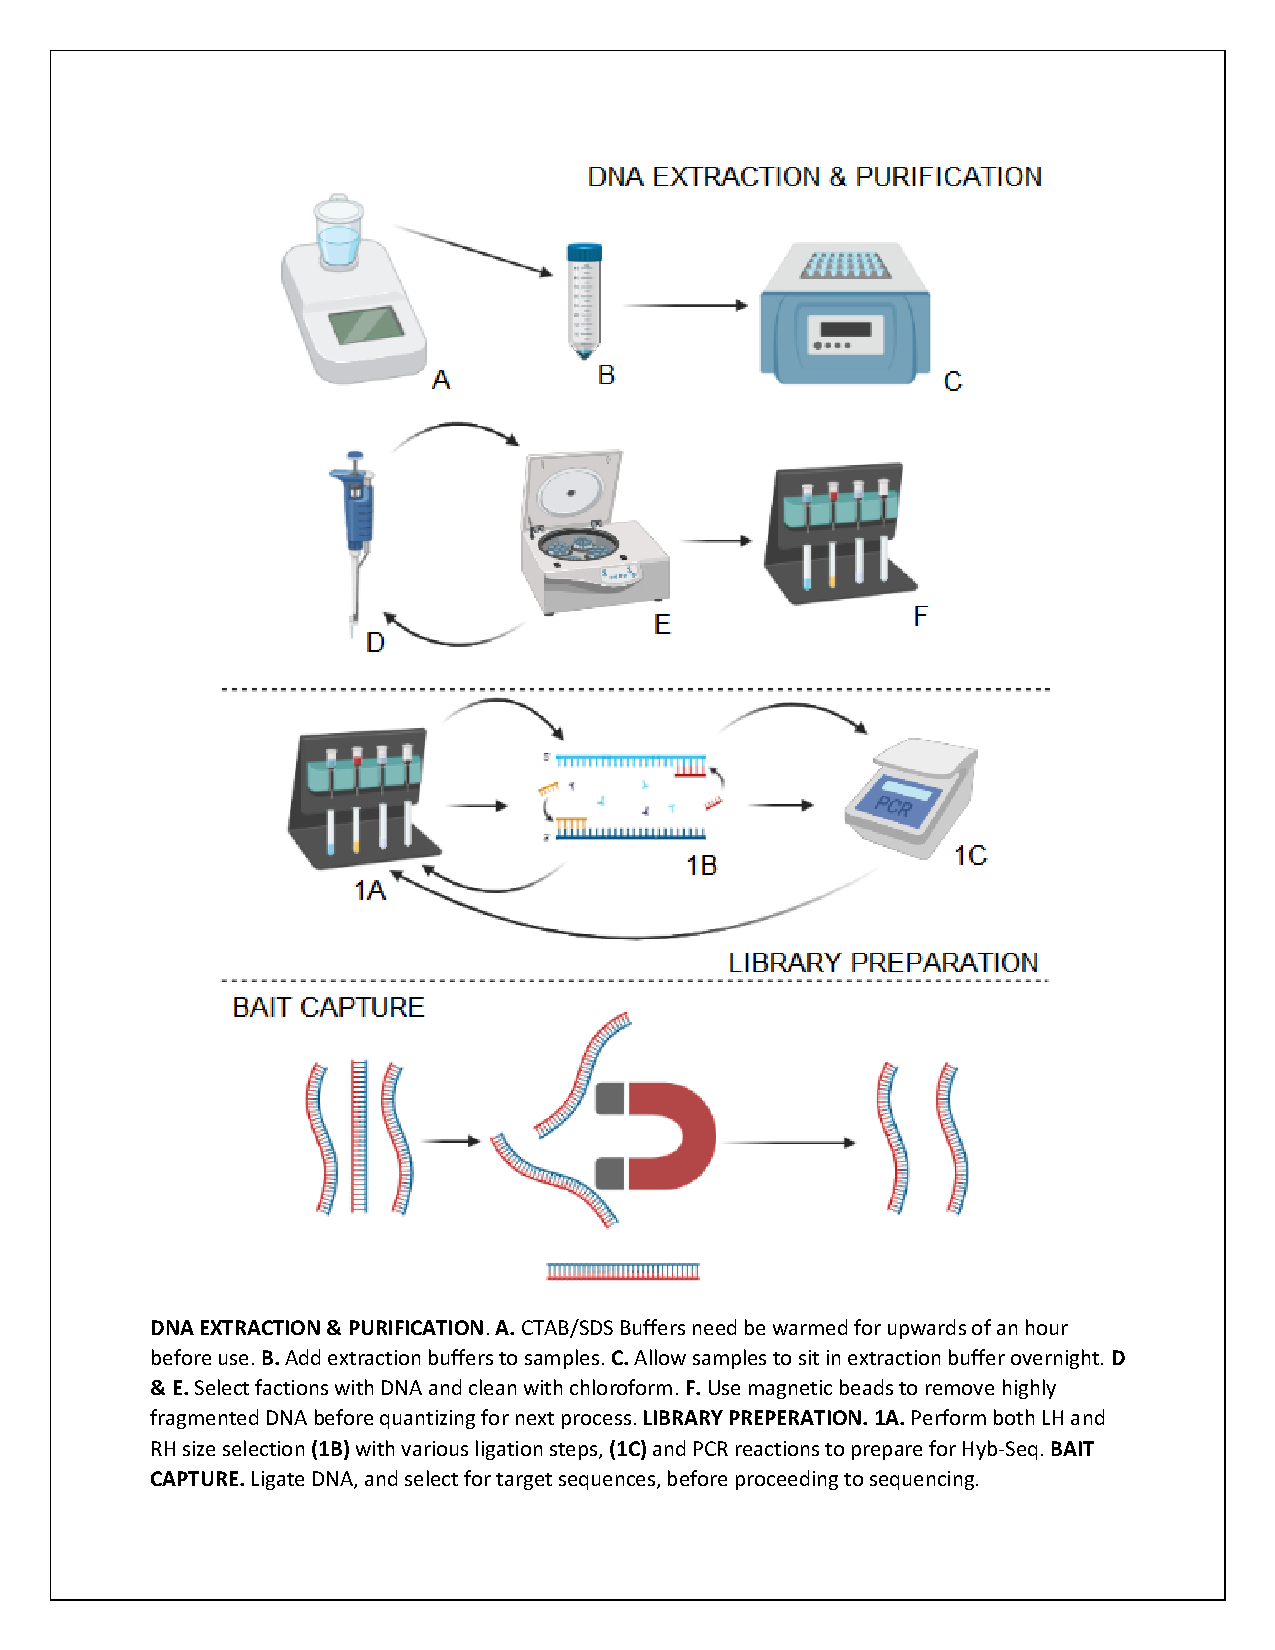
\includegraphics{../graphics/assorted/molecular_workflow.pdf}

\newpage

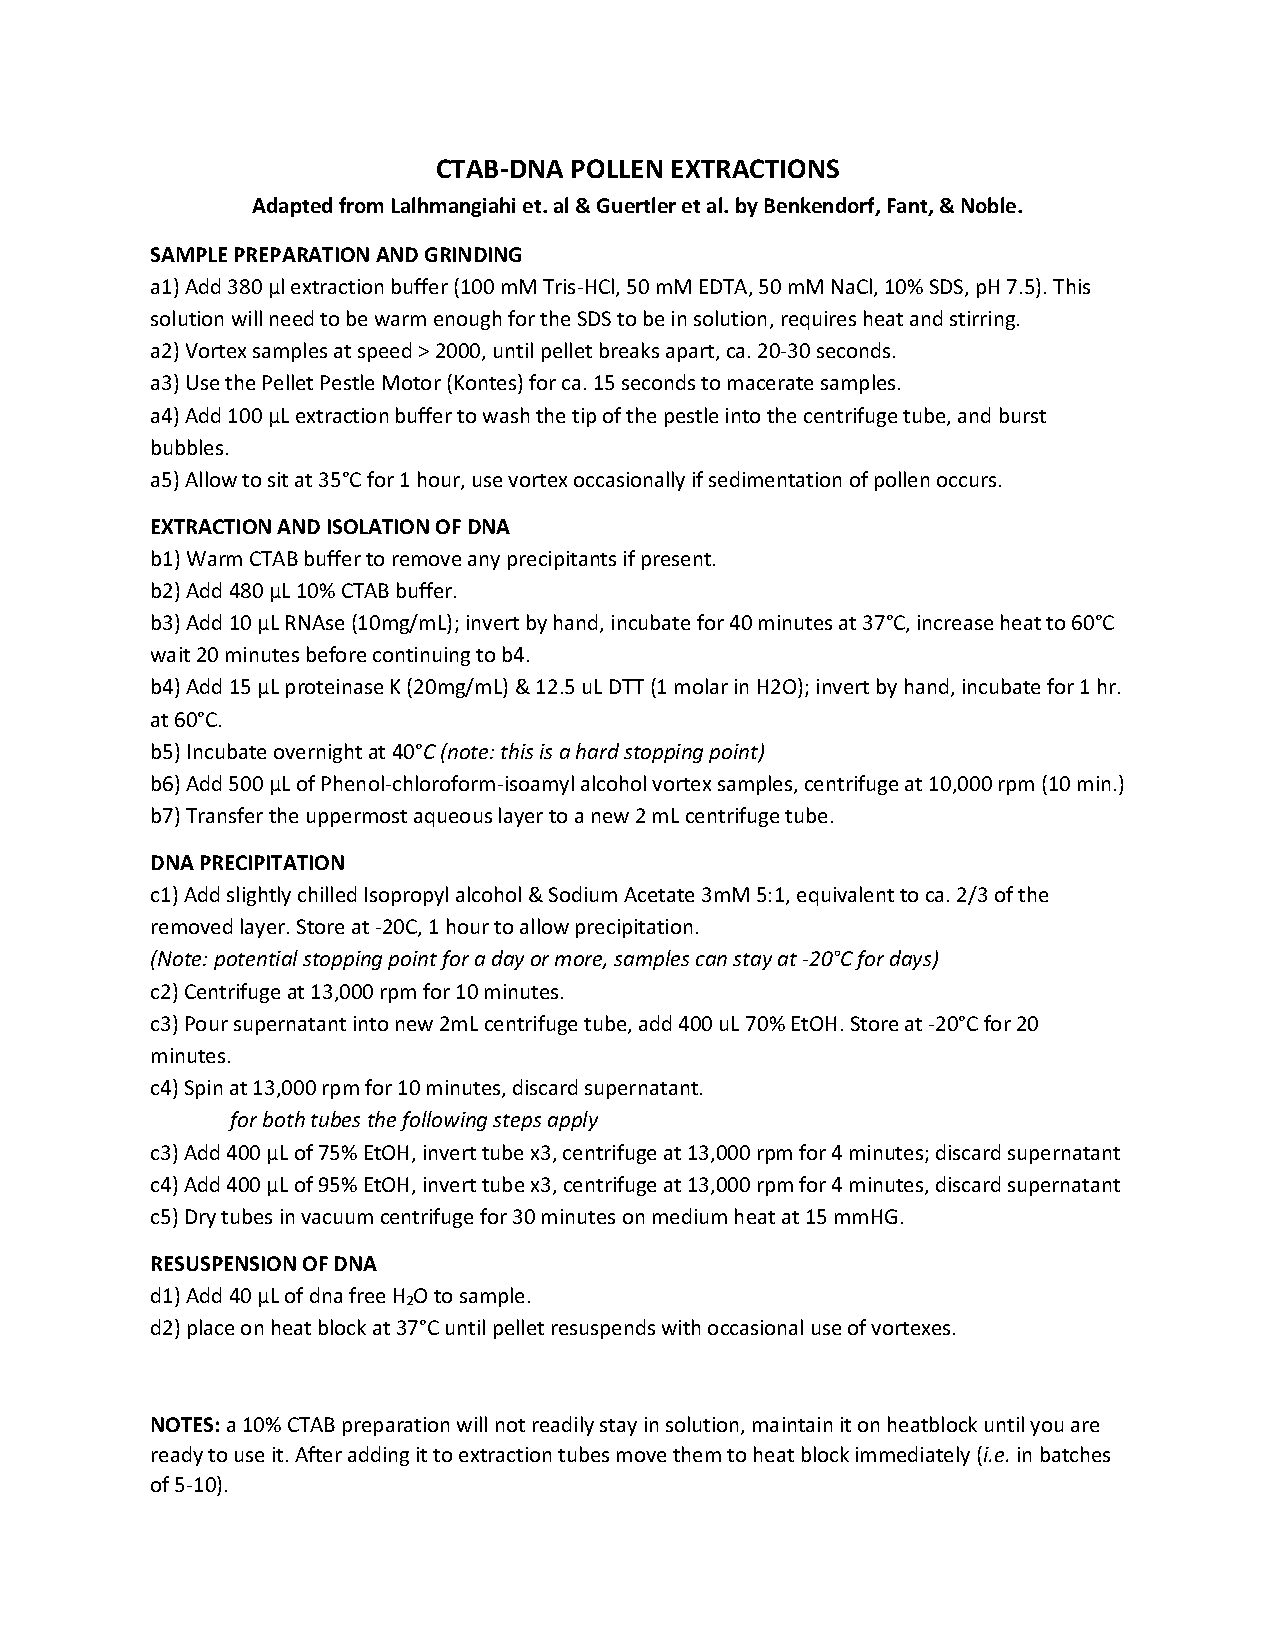
\includegraphics{../graphics/assorted/pollen_ctab.pdf}

\newpage

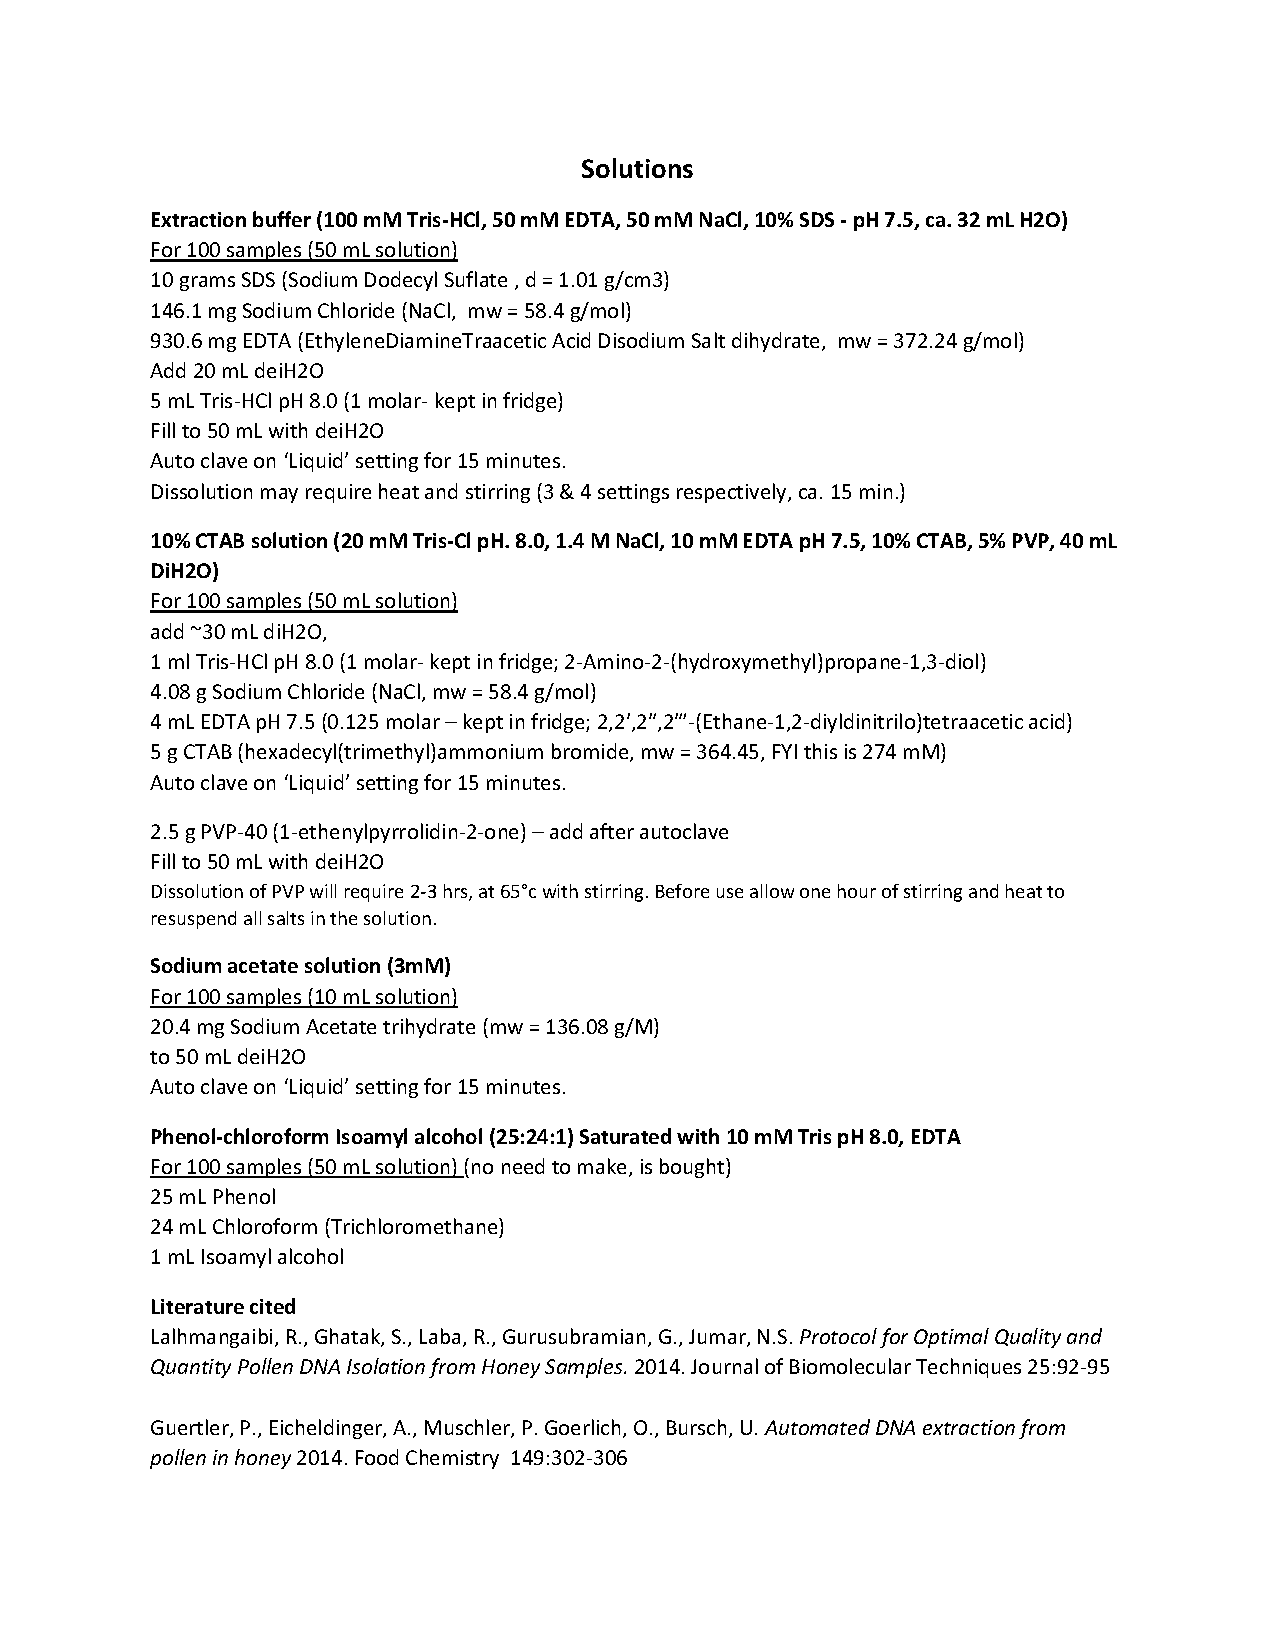
\includegraphics{../graphics/assorted/pollen_ctab-1.pdf}

\newpage

THIS SHOULD BE TURNED INTO A SMALLER PNG, AND HAVE THE NUMBER OF
SEQUENCED METAGENOMIC SAMPLES PLACED INTO THAT COLUMN AND INCLUDED IN
TEXT \textasciitilde\textasciitilde\textasciitilde{} NEED THIS !!!!

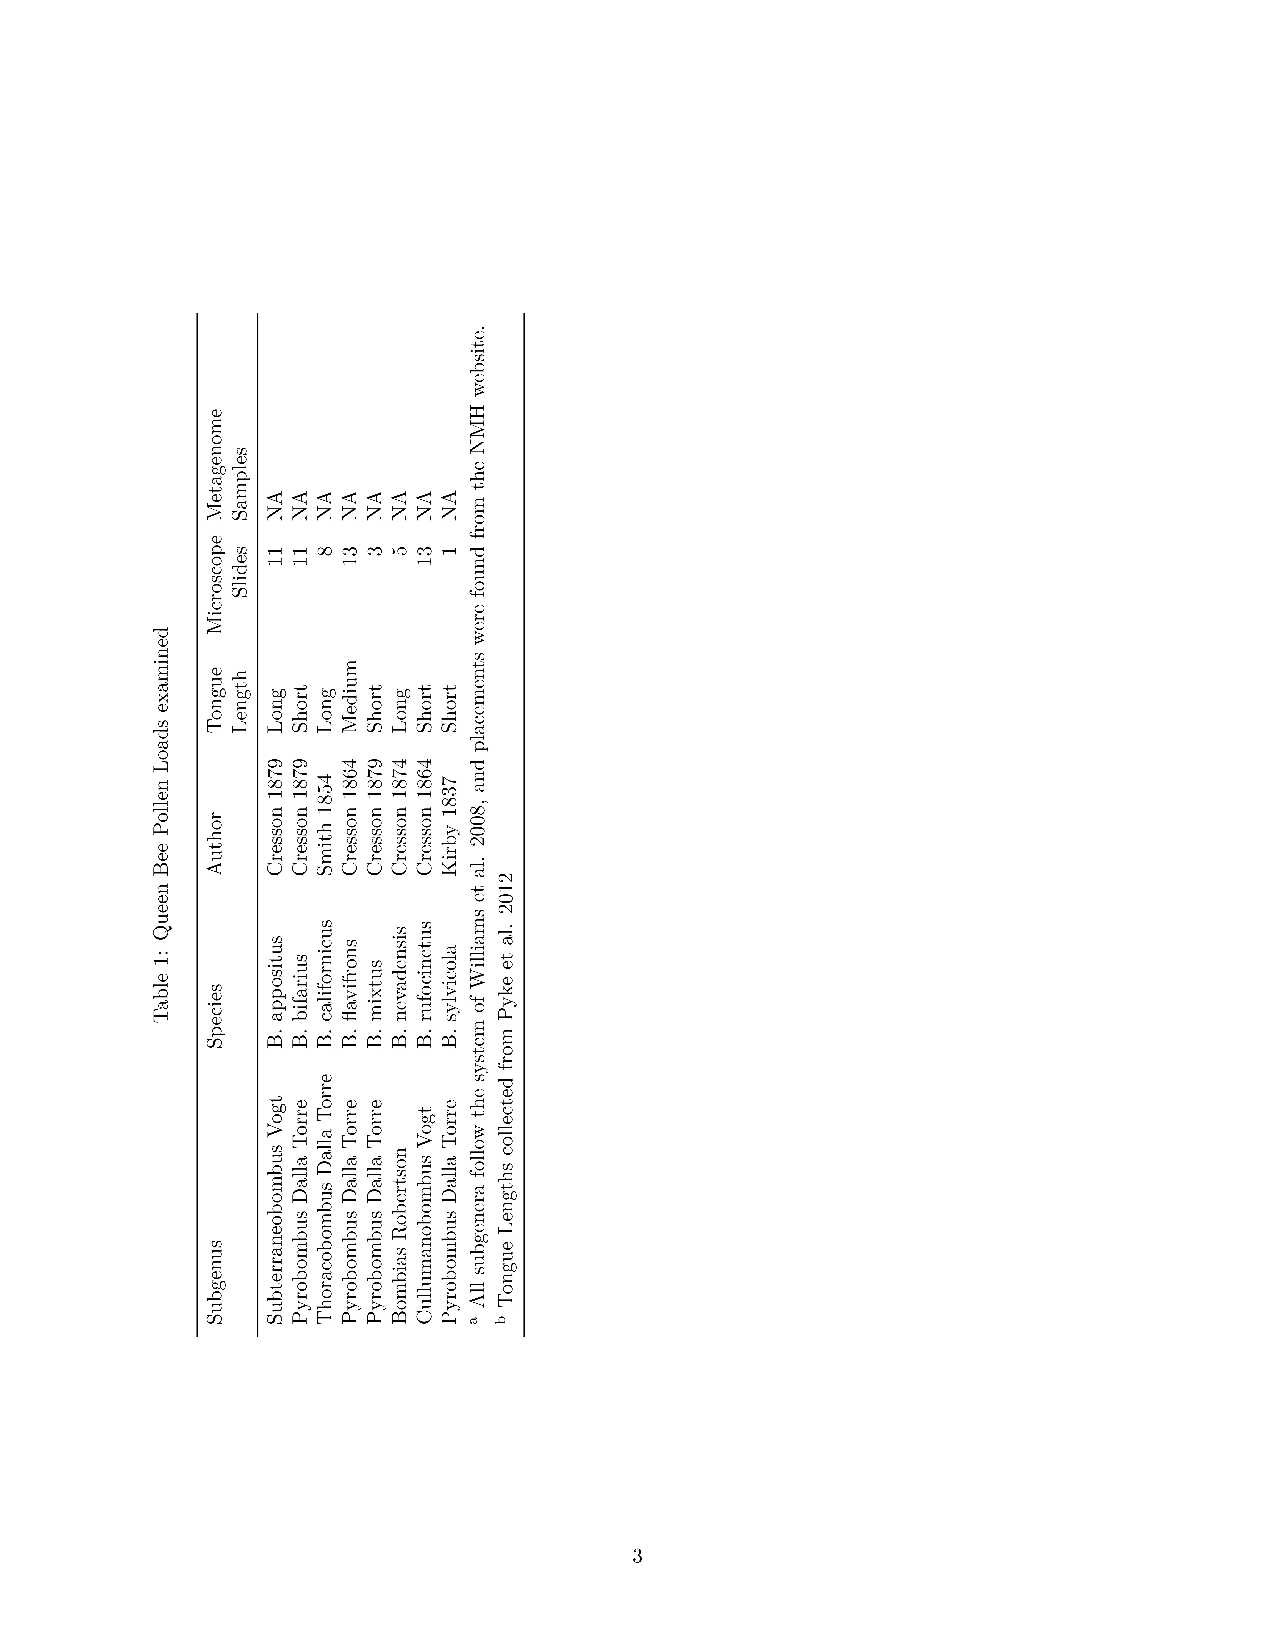
\includegraphics{../graphics/tables/bombus_samples.pdf}

\newpage

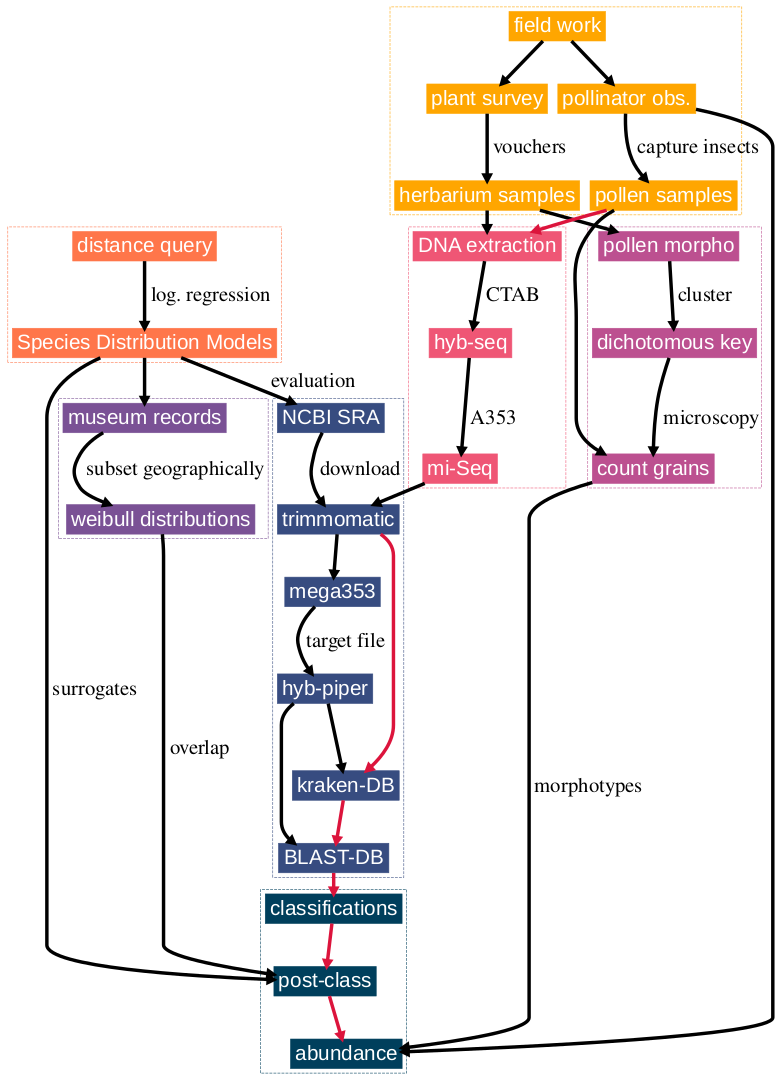
\includegraphics[width=5.83in,height=1.25\textheight]{../graphics/plots/flowchart}

\newpage

\hypertarget{references-1}{%
\section*{References}\label{references-1}}
\addcontentsline{toc}{section}{References}

\hypertarget{refs}{}
\begin{CSLReferences}{1}{0}
\leavevmode\vadjust pre{\hypertarget{ref-ackerfield2015flora}{}}%
Ackerfield, J. (2015). \emph{Flora of colorado}. BRIT Press Fort Worth.

\leavevmode\vadjust pre{\hypertarget{ref-alarcon2010congruence}{}}%
Alarcón, R. (2010). Congruence between visitation and pollen-transport
networks in a california plant--pollinator community. \emph{Oikos},
\textbf{119}, 35--44. Retrieved from
\url{https://onlinelibrary.wiley.com/doi/abs/10.1111/j.1600-0706.2009.17694.x}

\leavevmode\vadjust pre{\hypertarget{ref-aldous1919eradicating}{}}%
Aldous, A.E. (1919). \emph{Eradicating tall larkspur on cattle ranges in
the national forest}. US Department of Agriculture.

\leavevmode\vadjust pre{\hypertarget{ref-allouche2006assessing}{}}%
Allouche, O., Tsoar, A. \& Kadmon, R. (2006). Assessing the accuracy of
species distribution models: Prevalence, kappa and the true skill
statistic (TSS). \emph{Journal of applied ecology}, \textbf{43},
1223--1232.

\leavevmode\vadjust pre{\hypertarget{ref-allred2012flora}{}}%
Allred, K.W. \& Ivey, R. (2012). Flora neomexicana III: An illustrated
identification manual. \emph{Lulu. com}.

\leavevmode\vadjust pre{\hypertarget{ref-araujo2007ensemble}{}}%
Araujo, M.B. \& New, M. (2007). Ensemble forecasting of species
distributions. \emph{Trends in ecology \& evolution}, \textbf{22},
42--47.

\leavevmode\vadjust pre{\hypertarget{ref-augspurger2020concordance}{}}%
Augspurger, C.K. \& Zaya, D.N. (2020). Concordance of long-term shifts
with climate warming varies among phenological events and herbaceous
species. \emph{Ecological Monographs}, \textbf{90}, e01421.

\leavevmode\vadjust pre{\hypertarget{ref-baker2021PAFTOL}{}}%
Baker, W.J., Bailey, P., Barber, V., Barker, A., Bellot, S., Bishop, D.,
Botigué, L.R., Brewer, G., Carruthers, T., Clarkson, J.J., Cook, J.,
Cowan, R.S., Dodsworth, S., Epitawalage, N., Françoso, E., Gallego, B.,
Johnson, M.G., Kim, J.T., Leempoel, K., Maurin, O., Mcginnie, C.,
Pokorny, L., Roy, S., Stone, M., Toledo, E., Wickett, N.J., Zuntini,
A.R., Eiserhardt, W.L., Kersey, P.J., Leitch, I.J. \& Forest, F.
(2021a). {A Comprehensive Phylogenomic Platform for Exploring the
Angiosperm Tree of Life}. \emph{Systematic Biology}, \textbf{71},
301--319. Retrieved from \url{https://doi.org/10.1093/sysbio/syab035}

\leavevmode\vadjust pre{\hypertarget{ref-baker2021exploring}{}}%
Baker, W., Dodsworth, S., Forest, F., Graham, S., Johnson, M.,
McDonnell, A., Pokorny, L., Tate, J., Wicke, S. \& Wickett, N. (2021b).
\href{https://doi.org/10.1002/ajb2.1703}{Exploring Angiosperms353: An
open, community toolkit for collaborative phylogenomic research on
flowering plants}. \emph{American Journal of Botany}, \textbf{108}.

\leavevmode\vadjust pre{\hypertarget{ref-barbet2012selecting}{}}%
Barbet-Massin, M., Jiguet, F., Albert, C.H. \& Thuiller, W. (2012).
Selecting pseudo-absences for species distribution models: How, where
and how many? \emph{Methods in ecology and evolution}, \textbf{3},
327--338.

\leavevmode\vadjust pre{\hypertarget{ref-barker2021pollen}{}}%
Barker, D.A. \& Arceo-Gomez, G. (2021). {Pollen transport networks
reveal highly diverse and temporally stable plant--pollinator
interactions in an Appalachian floral community}. \emph{AoB PLANTS},
\textbf{13}. Retrieved from \url{https://doi.org/10.1093/aobpla/plab062}

\leavevmode\vadjust pre{\hypertarget{ref-basey2015producing}{}}%
Basey, A.C., Fant, J.B. \& Kramer, A.T. (2015). Producing native plant
materials for restoration: 10 rules to collect and maintain genetic
diversity. \emph{Native Plants Journal}, \textbf{16}, 37--53.

\leavevmode\vadjust pre{\hypertarget{ref-beattie1971technique}{}}%
Beattie, A. (1971). A technique for the study of insect-borne pollen.
\emph{The Pan-Pacific Entomologist}, \textbf{47}, 82.

\leavevmode\vadjust pre{\hypertarget{ref-beck2021palmer}{}}%
Beck, J.B., Markley, M.L., Zielke, M.G., Thomas, J.R., Hale, H.J.,
Williams, L.D. \& Johnson, M.G. (2021). Are palmer's elm-leaf goldenrod
and the smooth elm-leaf goldenrod real? The Angiosperms353 kit provides
within-species signal in solidago ulmifolia sl. \emph{Systematic
Botany}, \textbf{46}, 1107--1113.

\leavevmode\vadjust pre{\hypertarget{ref-belitz2020accuracy}{}}%
Belitz, M.W., Larsen, E.A., Ries, L. \& Guralnick, R.P. (2020). The
accuracy of phenology estimators for use with sparsely sampled
presence-only observations. \emph{Methods in Ecology and Evolution},
\textbf{11}, 1273--1285.

\leavevmode\vadjust pre{\hypertarget{ref-bell2019quantitative}{}}%
Bell, K.L., Burgess, K.S., Botsch, J.C., Dobbs, E.K., Read, T.D. \&
Brosi, B.J. (2019). Quantitative and qualitative assessment of pollen
DNA metabarcoding using constructed species mixtures. \emph{Molecular
Ecology}, \textbf{28}, 431--455.

\leavevmode\vadjust pre{\hypertarget{ref-bell2017applying}{}}%
Bell, K.L., Fowler, J., Burgess, K.S., Dobbs, E.K., Gruenewald, D.,
Lawley, B., Morozumi, C. \& Brosi, B.J. (2017). Applying pollen DNA
metabarcoding to the study of plant--pollinator interactions.
\emph{Applications in plant sciences}, \textbf{5}, 1600124.

\leavevmode\vadjust pre{\hypertarget{ref-bell2021comparing}{}}%
Bell, K.L., Petit III, R.A., Cutler, A., Dobbs, E.K., Macpherson, J.M.,
Read, T.D., Burgess, K.S. \& Brosi, B.J. (2021). Comparing whole-genome
shotgun sequencing and DNA metabarcoding approaches for species
identification and quantification of pollen species mixtures.
\emph{Ecology and Evolution}, \textbf{11}, 16082--16098.

\leavevmode\vadjust pre{\hypertarget{ref-bell2022plants}{}}%
Bell, K.L., Turo, K.J., Lowe, A., Nota, K., Keller, A., Encinas-Viso,
F., Parducci, L., Richardson, R.T., Leggett, R.M., Brosi, B.J. \&
others. (2022). Plants, pollinators and their interactions under global
ecological change: The role of pollen DNA metabarcoding. \emph{Molecular
ecology}.

\leavevmode\vadjust pre{\hypertarget{ref-belsky1999survey}{}}%
Belsky, A.J., Matzke, A. \& Uselman, S. (1999). Survey of livestock
influences on stream and riparian ecosystems in the western united
states. \emph{Journal of Soil and water Conservation}, \textbf{54},
419--431.

\leavevmode\vadjust pre{\hypertarget{ref-bergman1996micrometeorological}{}}%
Bergman, P., Molau, U. \& Holmgren, B. (1996). Micrometeorological
impacts on insect activity and plant reproductive success in an alpine
environment, swedish lapland. \emph{Arctic and alpine research},
\textbf{28}, 196--202.

\leavevmode\vadjust pre{\hypertarget{ref-betancourt2005implementing}{}}%
Betancourt, J.L., Schwartz, M.D., Breshears, D.D., Cayan, D.R.,
Dettinger, M.D., Inouye, D.W., Post, E. \& Reed, B.C. (2005).
Implementing a US national phenology network.

\leavevmode\vadjust pre{\hypertarget{ref-bingham1998efficient}{}}%
Bingham, R.A. \& Orthner, A.R. (1998). Efficient pollination of alpine
plants. \emph{Nature}, \textbf{391}, 238--239.

\leavevmode\vadjust pre{\hypertarget{ref-bolger2014trimmomatic}{}}%
Bolger, A. \& Giorgi, F. (2014). Trimmomatic: A flexible read trimming
tool for illumina NGS data. \emph{Bioinformatics}, \textbf{30},
2114--2120.

\leavevmode\vadjust pre{\hypertarget{ref-bontvsutvsnaja2021bumble}{}}%
Bontsutsnaja, A., Karise, R., Mand, M. \& Smagghe, G. (2021). Bumble bee
foraged pollen analyses in spring time in southern estonia shows
abundant food sources. \emph{Insects}, \textbf{12}, 922.

\leavevmode\vadjust pre{\hypertarget{ref-bortolus2008error}{}}%
Bortolus, A. (2008). Error cascades in the biological sciences: The
unwanted consequences of using bad taxonomy in ecology. \emph{AMBIO: A
journal of the human environment}, \textbf{37}, 114--118.

\leavevmode\vadjust pre{\hypertarget{ref-brewen202176}{}}%
Brewen, C.J., Berrill, J.-P., Ritchie, M.W., Boston, K., Dagley, C.M.,
Jones, B., Coppoletta, M. \& Burnett, C.L. (2021). 76-year decline and
recovery of aspen mediated by contrasting fire regimes: Long-unburned,
infrequent and frequent mixed-severity wildfire. \emph{Plos one},
\textbf{16}, e0232995.

\leavevmode\vadjust pre{\hypertarget{ref-brito2018climate}{}}%
Brito-Morales, I., Molinos, J.G., Schoeman, D.S., Burrows, M.T.,
Poloczanska, E.S., Brown, C.J., Ferrier, S., Harwood, T.D., Klein, C.J.,
McDonald-Madden, E. \& others. (2018). Climate velocity can inform
conservation in a warming world. \emph{Trends in ecology \& evolution},
\textbf{33}, 441--457.

\leavevmode\vadjust pre{\hypertarget{ref-brosi2013single}{}}%
Brosi, B.J. \& Briggs, H.M. (2013). Single pollinator species losses
reduce floral fidelity and plant reproductive function.
\emph{Proceedings of the National Academy of Sciences}, \textbf{110},
13044--13048.

\leavevmode\vadjust pre{\hypertarget{ref-calabrese2014stacking}{}}%
Calabrese, J.M., Certain, G., Kraan, C. \& Dormann, C.F. (2014).
Stacking species distribution models and adjusting bias by linking them
to macroecological models. \emph{Global Ecology and Biogeography},
\textbf{23}, 99--112.

\leavevmode\vadjust pre{\hypertarget{ref-camacho2009blast}{}}%
Camacho, C., Coulouris, G., Avagyan, V., Ma, N., Papadopoulos, J.,
Bealer, K. \& Madden, T.L. (2009). BLAST+: Architecture and
applications. \emph{BMC bioinformatics}, \textbf{10}, 1--9.

\leavevmode\vadjust pre{\hypertarget{ref-cameron2020global}{}}%
Cameron, S.A. \& Sadd, B.M. (2020). Global trends in bumble bee health.
\emph{Annual review of entomology}, \textbf{65}, 209--232.

\leavevmode\vadjust pre{\hypertarget{ref-caradonna2021seeing}{}}%
CaraDonna, P.J., Burkle, L.A., Schwarz, B., Resasco, J., Knight, T.M.,
Benadi, G., Bluthgen, N., Dormann, C.F., Fang, Q., Frund, J. \& others.
(2021). Seeing through the static: The temporal dimension of
plant--animal mutualistic interactions. \emph{Ecology Letters},
\textbf{24}, 149--161.

\leavevmode\vadjust pre{\hypertarget{ref-caradonna2014shifts}{}}%
CaraDonna, P.J., Iler, A.M. \& Inouye, D.W. (2014). Shifts in flowering
phenology reshape a subalpine plant community. \emph{Proceedings of the
National Academy of Sciences}, \textbf{111}, 4916--4921.

\leavevmode\vadjust pre{\hypertarget{ref-caradonna2017interaction}{}}%
CaraDonna, P.J., Petry, W.K., Brennan, R.M., Cunningham, J.L.,
Bronstein, J.L., Waser, N.M. \& Sanders, N.J. (2017). Interaction
rewiring and the rapid turnover of plant--pollinator networks.
\emph{Ecology letters}, \textbf{20}, 385--394.

\leavevmode\vadjust pre{\hypertarget{ref-inextArticle}{}}%
Chao, A., Gotelli, N.J., Hsieh, T.C., Sande, E.L., Ma, K.H., Colwell,
R.K. \& Ellison, A.M. (2014). Rarefaction and extrapolation with hill
numbers: A framework for sampling and estimation in species diversity
studies. \emph{Ecological Monographs}, \textbf{84}, 45--67.

\leavevmode\vadjust pre{\hypertarget{ref-cheng2018tenkp}{}}%
Cheng, S., Melkonian, M., Smith, S.A., Brockington, S., Archibald, J.M.,
Delaux, P.-M., Li, F.-W., Melkonian, B., Mavrodiev, E.V., Sun, W., Fu,
Y., Yang, H., Soltis, D.E., Graham, S.W., Soltis, P.S., Liu, X., Xu, X.
\& Wong, G.K.-S. (2018). {10KP: A phylodiverse genome sequencing plan}.
\emph{GigaScience}, \textbf{7}. Retrieved from
\url{https://doi.org/10.1093/gigascience/giy013}

\leavevmode\vadjust pre{\hypertarget{ref-coissac2016barcodes}{}}%
Coissac, E., Hollingsworth, P.M., Lavergne, S. \& Taberlet, P. (2016).
From barcodes to genomes: Extending the concept of DNA barcoding.

\leavevmode\vadjust pre{\hypertarget{ref-coissac2012bioinformatic}{}}%
Coissac, E., Riaz, T. \& Puillandre, N. (2012). Bioinformatic challenges
for DNA metabarcoding of plants and animals. \emph{Molecular ecology},
\textbf{21}, 1834--1847.

\leavevmode\vadjust pre{\hypertarget{ref-colla2012assessing}{}}%
Colla, S.R., Gadallah, F., Richardson, L., Wagner, D. \& Gall, L.
(2012). Assessing declines of north american bumble bees (bombus spp.)
Using museum specimens. \emph{Biodiversity and Conservation},
\textbf{21}, 3585--3595.

\leavevmode\vadjust pre{\hypertarget{ref-cooke1976arroyos}{}}%
Cooke, R.U. \& Reeves, R.W. (1976). \emph{Arroyos and environmental
change in the american south-west}. Clarendon Press.

\leavevmode\vadjust pre{\hypertarget{ref-crisci2020end}{}}%
Crisci, J.V., Katinas, L., Apodaca, M.J. \& Hoch, P.C. (2020). The end
of botany. \emph{Trends in Plant Science}, \textbf{25}, 1173--1176.

\leavevmode\vadjust pre{\hypertarget{ref-cronquist1977intermountain}{}}%
Cronquist, A., Holmgren, A.H., Holmgren, N.H., Reveal, J.L., Holmgren,
P.K., Barneby, R \& others. (1977+). \emph{Intermountain flora. Vascular
plants of the intermountain west, USA volume six. The monocotyledons.}
Columbia University.

\leavevmode\vadjust pre{\hypertarget{ref-dahl1990wetlands}{}}%
Dahl, T.E. (1990). \emph{Wetlands losses in the united states, 1780's to
1980's}. US Department of the Interior, Fish; Wildlife Service.

\leavevmode\vadjust pre{\hypertarget{ref-davis2022new}{}}%
Davis, C.C., Lyra, G.M., Park, D.S., Asprino, R., Maruyama, R.,
Torquato, D., Cook, B.I. \& Ellison, A.M. (2022). New directions in
tropical phenology. \emph{Trends in Ecology \& Evolution}.

\leavevmode\vadjust pre{\hypertarget{ref-dobrowski2016climate}{}}%
Dobrowski, S.Z. \& Parks, S.A. (2016). Climate change velocity
underestimates climate change exposure in mountainous regions.
\emph{Nature Communications}, \textbf{7}, 1--8.

\leavevmode\vadjust pre{\hypertarget{ref-doylesCTAB}{}}%
Doyle, J.J. \& Doyle, J.L. (1987). A rapid DNA isolation procedure for
small quantities of fresh leaf tissue. \emph{Phytochemical Bulletin},
\textbf{19}, 11--15.

\leavevmode\vadjust pre{\hypertarget{ref-dubuis2011predicting}{}}%
Dubuis, A., Pottier, J., Rion, V., Pellissier, L., Theurillat, J.-P. \&
Guisan, A. (2011). Predicting spatial patterns of plant species
richness: A comparison of direct macroecological and species stacking
modelling approaches. \emph{Diversity and Distributions}, \textbf{17},
1122--1131.

\leavevmode\vadjust pre{\hypertarget{ref-elith2006novel}{}}%
Elith*, J., H. Graham*, C., P. Anderson, R., Dudik, M., Ferrier, S.,
Guisan, A., J. Hijmans, R., Huettmann, F., R. Leathwick, J., Lehmann, A.
\& others. (2006). Novel methods improve prediction of species'
distributions from occurrence data. \emph{Ecography}, \textbf{29},
129--151.

\leavevmode\vadjust pre{\hypertarget{ref-fazekas2009plant}{}}%
Fazekas, A.J., Kesanakurti, P.R., Burgess, K.S., Percy, D.M., Graham,
S.W., Barrett, S.C., Newmaster, S.G., Hajibabaei, M. \& Husband, B.C.
(2009). Are plant species inherently harder to discriminate than animal
species using DNA barcoding markers? \emph{Molecular Ecology Resources},
\textbf{9}, 130--139.

\leavevmode\vadjust pre{\hypertarget{ref-fenn2003ecological}{}}%
Fenn, M.E., Baron, J.S., Allen, E.B., Rueth, H.M., Nydick, K.R., Geiser,
L., Bowman, W.D., Sickman, J.O., Meixner, T., Johnson, D.W. \& others.
(2003). Ecological effects of nitrogen deposition in the western united
states. \emph{BioScience}, \textbf{53}, 404--420.

\leavevmode\vadjust pre{\hypertarget{ref-flora1993flora}{}}%
Flora of North America Editorial Committee, eds. (1993+). \emph{Flora of
north america north of mexico {[}online{]}}. Oxford University Press on
Demand.

\leavevmode\vadjust pre{\hypertarget{ref-fraser2007vpc}{}}%
Frase, Barbara A. \& Buck, P. (2007). {Vascular Plants of the Gothic
Area}. Retrieved from
\url{https://www.digitalrmbl.org/wp-content/uploads/2016/05/vascularplantlist_20071.pdf}

\leavevmode\vadjust pre{\hypertarget{ref-Gage2013HistoricalRO}{}}%
Gage, E. \& Cooper, D.J. (2013). Historical range of variation
assessment for wetland and riparian ecosystems, u.s. Forest service
rocky mountain region

\leavevmode\vadjust pre{\hypertarget{ref-goulson2010bumblebees}{}}%
Goulson, D. (2010). \emph{Bumblebees: Behaviour, ecology, and
conservation}. Oxford University Press on Demand.

\leavevmode\vadjust pre{\hypertarget{ref-goulson2005causes}{}}%
Goulson, D., Hanley, M.E., Darvill, B., Ellis, J. \& Knight, M.E.
(2005). Causes of rarity in bumblebees. \emph{Biological conservation},
\textbf{122}, 1--8.

\leavevmode\vadjust pre{\hypertarget{ref-goulson2008decline}{}}%
Goulson, D., Lye, G. \& Darvill, B. (2008). The decline and conservation
of bumblebees. \emph{Annual review of entomology}, \textbf{53},
191--208.

\leavevmode\vadjust pre{\hypertarget{ref-grixti2009decline}{}}%
Grixti, J.C., Wong, L.T., Cameron, S.A. \& Favret, C. (2009). Decline of
bumble bees (bombus) in the north american midwest. \emph{Biological
conservation}, \textbf{142}, 75--84.

\leavevmode\vadjust pre{\hypertarget{ref-cbol2009dna}{}}%
Group, C.P.W., Hollingsworth, P.M., Forrest, L.L., Spouge, J.L.,
Hajibabaei, M., Ratnasingham, S., Bank, M. van der, Chase, M.W., Cowan,
R.S., Erickson, D.L. \& others. (2009). A DNA barcode for land plants.
\emph{Proceedings of the National Academy of Sciences}, \textbf{106},
12794--12797.

\leavevmode\vadjust pre{\hypertarget{ref-china2011comparative}{}}%
Group, C.P.B., Li, D.-Z., Gao, L.-M., Li, H.-T., Wang, H., Ge, X.-J.,
Liu, J.-Q., Chen, Z.-D., Zhou, S.-L., Chen, S.-L. \& others. (2011).
Comparative analysis of a large dataset indicates that internal
transcribed spacer (ITS) should be incorporated into the core barcode
for seed plants. \emph{Proceedings of the National Academy of Sciences},
\textbf{108}, 19641--19646.

\leavevmode\vadjust pre{\hypertarget{ref-havens2007chicago}{}}%
Havens, K., Vitt, P., Schwarz, J., Orr, B. \& Crimmins, T. (2007).
Chicago botanic garden's conservation and outreach efforts on climate
change. \emph{BGjournal}, \textbf{4}, 13--16.

\leavevmode\vadjust pre{\hypertarget{ref-hebert2003biological}{}}%
Hebert, P.D., Cywinska, A., Ball, S.L. \& DeWaard, J.R. (2003).
Biological identifications through DNA barcodes. \emph{Proceedings of
the Royal Society of London. Series B: Biological Sciences},
\textbf{270}, 313--321.

\leavevmode\vadjust pre{\hypertarget{ref-hengl2017soilgrids250m}{}}%
Hengl, T., Mendes de Jesus, J., Heuvelink, G.B., Ruiperez Gonzalez, M.,
Kilibarda, M., Blagotić, A., Shangguan, W., Wright, M.N., Geng, X.,
Bauer-Marschallinger, B. \& others. (2017). SoilGrids250m: Global
gridded soil information based on machine learning. \emph{PLoS one},
\textbf{12}, e0169748.

\leavevmode\vadjust pre{\hypertarget{ref-fpc2022}{}}%
Hennig, C. (2020). \emph{Fpc: Flexible procedures for clustering}.
Retrieved from \url{https://CRAN.R-project.org/package=fpc}

\leavevmode\vadjust pre{\hypertarget{ref-hinchliff2015synthesis}{}}%
Hinchliff, C.E., Smith, S.A., Allman, J.F., Burleigh, J.G., Chaudhary,
R., Coghill, L.M., Crandall, K.A., Deng, J., Drew, B.T., Gazis, R. \&
others. (2015). Synthesis of phylogeny and taxonomy into a comprehensive
tree of life. \emph{Proceedings of the National Academy of Sciences},
\textbf{112}, 12764--12769.

\leavevmode\vadjust pre{\hypertarget{ref-hitchcock2018flora}{}}%
Hitchcock, C.L. \& Cronquist, A. (2018). \emph{Flora of the pacific
northwest: An illustrated manual}. University of Washington Press.

\leavevmode\vadjust pre{\hypertarget{ref-hollingsworth2016telling}{}}%
Hollingsworth, P.M., Li, D.-Z., Bank, M. van der \& Twyford, A.D.
(2016). Telling plant species apart with DNA: From barcodes to genomes.
\emph{Philosophical Transactions of the Royal Society B: Biological
Sciences}, \textbf{371}, 20150338.

\leavevmode\vadjust pre{\hypertarget{ref-inextPackage}{}}%
Hsieh, T.C., Ma, K.H. \& Chao, A. (2020). \emph{iNEXT: Interpolation and
extrapolation for species diversity}. Retrieved from
\url{http://chao.stat.nthu.edu.tw/wordpress/software_download/}

\leavevmode\vadjust pre{\hypertarget{ref-iler2021conceptual}{}}%
Iler, A.M., Humphrey, P.T., Ogilvie, J.E. \& CaraDonna, P.J. (2021).
Conceptual and practical issues limit the utility of statistical
estimators of phenological events. \emph{Ecosphere}, \textbf{12},
e03828.

\leavevmode\vadjust pre{\hypertarget{ref-janzen1967synchronization}{}}%
Janzen, D.H. (1967). Synchronization of sexual reproduction of trees
within the dry season in central america. \emph{Evolution}, \textbf{21},
620--637.

\leavevmode\vadjust pre{\hypertarget{ref-janzen2017nuclear}{}}%
Janzen, D.H., Burns, J.M., Cong, Q., Hallwachs, W., Dapkey, T.,
Manjunath, R., Hajibabaei, M., Hebert, P.D. \& Grishin, N.V. (2017).
Nuclear genomes distinguish cryptic species suggested by their DNA
barcodes and ecology. \emph{Proceedings of the National Academy of
Sciences}, \textbf{114}, 8313--8318.

\leavevmode\vadjust pre{\hypertarget{ref-jepson2022online}{}}%
\emph{Jepson flora project}. (2020).

\leavevmode\vadjust pre{\hypertarget{ref-johnson2021airborne}{}}%
Johnson, M.D., Fokar, M., Cox, R.D. \& Barnes, M.A. (2021). Airborne
environmental DNA metabarcoding detects more diversity, with less
sampling effort, than a traditional plant community survey. \emph{BMC
Ecology and Evolution}, \textbf{21}, 1--15.

\leavevmode\vadjust pre{\hypertarget{ref-johnson2016hybpiper}{}}%
Johnson, M.G., Gardner, E.M., Liu, Y., Medina, R., Goffinet, B., Shaw,
A.J., Zerega, N.J. \& Wickett, N.J. (2016). HybPiper: Extracting coding
sequence and introns for phylogenetics from high-throughput sequencing
reads using target enrichment. \emph{Applications in plant sciences},
\textbf{4}, 1600016.

\leavevmode\vadjust pre{\hypertarget{ref-johnson2019universal}{}}%
Johnson, M.G., Pokorny, L., Dodsworth, S., Botigue, L.R., Cowan, R.S.,
Devault, A., Eiserhardt, W.L., Epitawalage, N., Forest, F., Kim, J.T. \&
others. (2019). A universal probe set for targeted sequencing of 353
nuclear genes from any flowering plant designed using k-medoids
clustering. \emph{Systematic biology}, \textbf{68}, 594--606.

\leavevmode\vadjust pre{\hypertarget{ref-joshi2001local}{}}%
Joshi, J., Schmid, B., Caldeira, M., Dimitrakopoulos, P., Good, J.,
Harris, R., Hector, A., Huss-Danell, K., Jumpponen, A., Minns, A. \&
others. (2001). Local adaptation enhances performance of common plant
species. \emph{Ecology Letters}, \textbf{4}, 536--544.

\leavevmode\vadjust pre{\hypertarget{ref-keane2002cascading}{}}%
Keane, R.E. (2002). Cascading effects of fire exclusion in rocky
mountain ecosystems: A literature review.

\leavevmode\vadjust pre{\hypertarget{ref-kearns2001natural}{}}%
Kearns, C.A., Thomson, J.D. \& others. (2001). \emph{Natural history of
bumblebees}. University Press of Colorado.

\leavevmode\vadjust pre{\hypertarget{ref-kramer2015report}{}}%
Kramer, A.T. \& Havens, K. (2015). Report in brief: Assessing botanical
capacity to address grand challenges in the united states. \emph{Natural
Areas Journal}, \textbf{35}, 83--89.

\leavevmode\vadjust pre{\hypertarget{ref-kress2017plant}{}}%
Kress, W.J. (2017). Plant DNA barcodes: Applications today and in the
future. \emph{Journal of systematics and evolution}, \textbf{55},
291--307.

\leavevmode\vadjust pre{\hypertarget{ref-kress2007two}{}}%
Kress, W.J. \& Erickson, D.L. (2007). A two-locus global DNA barcode for
land plants: The coding rbcL gene complements the non-coding trnH-psbA
spacer region. \emph{PLoS one}, \textbf{2}, e508.

\leavevmode\vadjust pre{\hypertarget{ref-caret}{}}%
Kuhn, M. (2022). \emph{Caret: Classification and regression training}.
Retrieved from \url{https://CRAN.R-project.org/package=caret}

\leavevmode\vadjust pre{\hypertarget{ref-lamb2019quantitative}{}}%
Lamb, P.D., Hunter, E., Pinnegar, J.K., Creer, S., Davies, R.G. \&
Taylor, M.I. (2019). How quantitative is metabarcoding: A
meta-analytical approach. \emph{Molecular ecology}, \textbf{28},
420--430.

\leavevmode\vadjust pre{\hypertarget{ref-aim2019database}{}}%
Land Management, B. of. (2019). U.s. Department of interior bureau of
land management, BLM - assessment, inventory, and monitoring (AIM)
terrestrial indicators raw dataset. Retrieved from
\url{https://gbp-blm-egis.hub.arcgis.com/pages/aim}

\leavevmode\vadjust pre{\hypertarget{ref-lang2019genome}{}}%
Lang, D., Tang, M., Hu, J. \& Zhou, X. (2019). Genome-skimming provides
accurate quantification for pollen mixtures. \emph{Molecular Ecology
Resources}, \textbf{19}, 1433--1446.

\leavevmode\vadjust pre{\hypertarget{ref-lesica2012manual}{}}%
Lesica, P., Lavin, M. \& Stickney, P.F. (2012). \emph{Manual of montana
vascular plants}. Brit Press.

\leavevmode\vadjust pre{\hypertarget{ref-lewin2022biogenome}{}}%
Lewin, H.A., Richards, S., Aiden, E.L., Allende, M.L., Archibald, J.M.,
Bálint, M., Barker, K.B., Baumgartner, B., Belov, K., Bertorelle, G.,
Blaxter, M.L., Cai, J., Caperello, N.D., Carlson, K., Castilla-Rubio,
J.C., Chaw, S.-M., Chen, L., Childers, A.K., Coddington, J.A., Conde,
D.A., Corominas, M., Crandall, K.A., Crawford, A.J., DiPalma, F.,
Durbin, R., Ebenezer, T.E., Edwards, S.V., Fedrigo, O., Flicek, P.,
Formenti, G., Gibbs, R.A., Gilbert, M.T.P., Goldstein, M.M., Graves,
J.M., Greely, H.T., Grigoriev, I.V., Hackett, K.J., Hall, N., Haussler,
D., Helgen, K.M., Hogg, C.J., Isobe, S., Jakobsen, K.S., Janke, A.,
Jarvis, E.D., Johnson, W.E., Jones, S.J.M., Karlsson, E.K., Kersey,
P.J., Kim, J.-H., Kress, W.J., Kuraku, S., Lawniczak, M.K.N.,
Leebens-Mack, J.H., Li, X., Lindblad-Toh, K., Liu, X., Lopez, J.V.,
Marques-Bonet, T., Mazard, S., Mazet, J.A.K., Mazzoni, C.J., Myers,
E.W., O'Neill, R.J., Paez, S., Park, H., Robinson, G.E., Roquet, C.,
Ryder, O.A., Sabir, J.S.M., Shaffer, H.B., Shank, T.M., Sherkow, J.S.,
Soltis, P.S., Tang, B., Tedersoo, L., Uliano-Silva, M., Wang, K., Wei,
X., Wetzer, R., Wilson, J.L., Xu, X., Yang, H., Yoder, A.D. \& Zhang, G.
(2022). The earth BioGenome project 2020: Starting the clock.
\emph{Proceedings of the National Academy of Sciences}, \textbf{119},
e2115635118. Retrieved from
\url{https://www.pnas.org/doi/abs/10.1073/pnas.2115635118}

\leavevmode\vadjust pre{\hypertarget{ref-liang2021evolutionary}{}}%
Liang, H., Zhao, Y.-H., Rafferty, N.E., Ren, Z.-X., Zhong, L., Li,
H.-D., Li, D.-Z. \& Wang, H. (2021). Evolutionary and ecological factors
structure a plant--bumblebee network in a biodiversity hotspot, the
himalaya--hengduan mountains. \emph{Functional Ecology}, \textbf{35},
2523--2535.

\leavevmode\vadjust pre{\hypertarget{ref-darwin2022project}{}}%
Life Project Consortium, D.T. of, Blaxter, M., Mieszkowska, N., Palma,
F.D., Holland, P., Durbin, R., Richards, T., Berriman, M., Kersey, P.,
Hollingsworth, P., Wilson, W., Twyford, A., Gaya, E., Lawniczak, M.,
Lewis, O., Broad, G., Howe, K., Hart, M., Flicek, P. \& Barnes, I.
(2022). Sequence locally, think globally: The darwin tree of life
project. \emph{Proceedings of the National Academy of Sciences},
\textbf{119}, e2115642118. Retrieved from
\url{https://www.pnas.org/doi/abs/10.1073/pnas.2115642118}

\leavevmode\vadjust pre{\hypertarget{ref-li2016responses}{}}%
Li, X., Jiang, L., Meng, F., Wang, S., Niu, H., Iler, A.M., Duan, J.,
Zhang, Z., Luo, C., Cui, S. \& others. (2016). Responses of sequential
and hierarchical phenological events to warming and cooling in alpine
meadows. \emph{Nature Communications}, \textbf{7}, 1--8.

\leavevmode\vadjust pre{\hypertarget{ref-liu2014identification}{}}%
Liu, J., Shi, L., Han, J., Li, G., Lu, H., Hou, J., Zhou, X., Meng, F.
\& Downie, S.R. (2014). Identification of species in the angiosperm
family apiaceae using DNA barcodes. \emph{Molecular ecology resources},
\textbf{14}, 1231--1238.

\leavevmode\vadjust pre{\hypertarget{ref-li2015plant}{}}%
Li, X., Yang, Y., Henry, R.J., Rossetto, M., Wang, Y. \& Chen, S.
(2015). Plant DNA barcoding: From gene to genome. \emph{Biological
Reviews}, \textbf{90}, 157--166.

\leavevmode\vadjust pre{\hypertarget{ref-loarie2009velocity}{}}%
Loarie, S.R., Duffy, P.B., Hamilton, H., Asner, G.P., Field, C.B. \&
Ackerly, D.D. (2009). The velocity of climate change. \emph{Nature},
\textbf{462}, 1052--1055.

\leavevmode\vadjust pre{\hypertarget{ref-lu2017bracken}{}}%
Lu, J., Breitwieser, F.P., Thielen, P. \& Salzberg, S.L. (2017).
Bracken: Estimating species abundance in metagenomics data. \emph{PeerJ
Computer Science}, \textbf{3}, e104.

\leavevmode\vadjust pre{\hypertarget{ref-cluster2022}{}}%
Maechler, M., Rousseeuw, P., Struyf, A., Hubert, M. \& Hornik, K.
(2022). \emph{Cluster: Cluster analysis basics and extensions}.
Retrieved from \url{https://CRAN.R-project.org/package=cluster}

\leavevmode\vadjust pre{\hypertarget{ref-mainali2022alpha}{}}%
Mainali, K. \& Slud, E. (2022). \emph{CooccurrenceAffinity: Affinity in
cooccrrence data}.

\leavevmode\vadjust pre{\hypertarget{ref-mainali2022better}{}}%
Mainali, K.P., Slud, E., Singer, M.C. \& Fagan, W.F. (2022). A better
index for analysis of co-occurrence and similarity. \emph{Science
Advances}, \textbf{8}, eabj9204.

\leavevmode\vadjust pre{\hypertarget{ref-bien2022}{}}%
Maitner, B. (2022). \emph{BIEN: Tools for accessing the botanical
information and ecology network database}. Retrieved from
\url{https://CRAN.R-project.org/package=BIEN}

\leavevmode\vadjust pre{\hypertarget{ref-manzano2021flippant}{}}%
Manzano, S. (2021). Flippant attitudes towards plant identification
jeopardize early career botanists. \emph{Trends in Plant Science},
\textbf{26}, 987--988.

\leavevmode\vadjust pre{\hypertarget{ref-mclay2021new}{}}%
McLay, T.G., Birch, J.L., Gunn, B.F., Ning, W., Tate, J.A., Nauheimer,
L., Joyce, E.M., Simpson, L., Schmidt-Lebuhn, A.N., William J \& others.
(2021). New targets acquired: Improving locus recovery from the
Angiosperms353 probe set. \emph{Applications in plant sciences},
\textbf{9}.

\leavevmode\vadjust pre{\hypertarget{ref-mohlenbrock2002vascular}{}}%
Mohlenbrock, R.H. (2002). \emph{Vascular flora of illinois}. SIU Press.

\leavevmode\vadjust pre{\hypertarget{ref-moore2003its}{}}%
Moore, A.J. \& Bohs, L. (2003). An ITS phylogeny of balsamorhiza and
wyethia (asteraceae: heliantheae). \emph{American Journal of Botany},
\textbf{90}, 1653--1660.

\leavevmode\vadjust pre{\hypertarget{ref-naiman1988alteration}{}}%
Naiman, R.J., Johnston, C.A. \& Kelley, J.C. (1988). Alteration of north
american streams by beaver. \emph{BioScience}, \textbf{38}, 753--762.

\leavevmode\vadjust pre{\hypertarget{ref-sdmPackage}{}}%
Naimi, B. \& Araujo, M.B. (2016).
\href{https://doi.org/10.1111/ecog.01881}{Sdm: A reproducible and
extensible r platform for species distribution modelling}.
\emph{Ecography}, \textbf{39}, 368--375.

\leavevmode\vadjust pre{\hypertarget{ref-usdm2014}{}}%
Naimi, B., Hamm, N. a.s., Groen, T.A., Skidmore, A.K. \& Toxopeus, A.G.
(2014). \href{https://doi.org/10.1111/j.1600-0587.2013.00205.x}{Where is
positional uncertainty a problem for species distribution modelling}.
\emph{Ecography}, \textbf{37}, 191--203.

\leavevmode\vadjust pre{\hypertarget{ref-nazaire2014phylogenetic}{}}%
Nazaire, M. \& Hufford, L. (2014). Phylogenetic systematics of the genus
mertensia (boraginaceae). \emph{Systematic Botany}, \textbf{39},
268--303.

\leavevmode\vadjust pre{\hypertarget{ref-nevado2016widespread}{}}%
Nevado, B., Atchison, G.W., Hughes, C.E. \& Filatov, D.A. (2016).
Widespread adaptive evolution during repeated evolutionary radiations in
new world lupins. \emph{Nature communications}, \textbf{7}, 1--9.

\leavevmode\vadjust pre{\hypertarget{ref-Newstrom1994ANC}{}}%
Newstrom, L.E., Frankie, G.W. \& Baker, H.G. (1994). A new
classification for plant phenology based on flowering patterns in
lowland tropical rain forest trees at la selva, costa rica.
\emph{Biotropica}, \textbf{26}, 141--159.

\leavevmode\vadjust pre{\hypertarget{ref-oberhauser2015monarchs}{}}%
Oberhauser, K.S., Nail, K.R. \& Altizer, S. (2015). \emph{Monarchs in a
changing world: Biology and conservation of an iconic butterfly}.
Cornell University Press.

\leavevmode\vadjust pre{\hypertarget{ref-gbifDL2021sdms}{}}%
Occdownload Gbif.Org. (2021). Occurrence download. Retrieved from
\url{https://www.gbif.org/occurrence/download/0206948-200613084148143}

\leavevmode\vadjust pre{\hypertarget{ref-vegans2022}{}}%
Oksanen, J., Simpson, G.L., Blanchet, F.G., Kindt, R., Legendre, P.,
Minchin, P.R., O'Hara, R.B., Solymos, P., Stevens, M.H.H., Szoecs, E.,
Wagner, H., Barbour, M., Bedward, M., Bolker, B., Borcard, D., Carvalho,
G., Chirico, M., De Caceres, M., Durand, S., Evangelista, H.B.A.,
FitzJohn, R., Friendly, M., Furneaux, B., Hannigan, G., Hill, M.O.,
Lahti, L., McGlinn, D., Ouellette, M.-H., Ribeiro Cunha, E., Smith, T.,
Stier, A., Ter Braak, C.J.F. \& Weedon, J. (2022). \emph{Vegan:
Community ecology package}. Retrieved from
\url{https://CRAN.R-project.org/package=vegan}

\leavevmode\vadjust pre{\hypertarget{ref-oliver2009cryptic}{}}%
Oliver, P.M., Adams, M., Lee, M.S., Hutchinson, M.N. \& Doughty, P.
(2009). Cryptic diversity in vertebrates: Molecular data double
estimates of species diversity in a radiation of australian lizards
(diplodactylus, gekkota). \emph{Proceedings of the Royal Society B:
Biological Sciences}, \textbf{276}, 2001--2007.

\leavevmode\vadjust pre{\hypertarget{ref-omernik1987ecoregions}{}}%
Omernik, J.M. (1987). Ecoregions of the conterminous united states.
\emph{Annals of the Association of American geographers}, \textbf{77},
118--125.

\leavevmode\vadjust pre{\hypertarget{ref-ottenlips2021resolving}{}}%
Ottenlips, M.V., Mansfield, D.H., Buerki, S., Feist, M.A.E., Downie,
S.R., Dodsworth, S., Forest, F., Plunkett, G.M. \& Smith, J.F. (2021).
Resolving species boundaries in a recent radiation with the
Angiosperms353 probe set: The lomatium packardiae/l. Anomalum clade of
the l. Triternatum (apiaceae) complex. \emph{American journal of
botany}, \textbf{108}, 1217--1233.

\leavevmode\vadjust pre{\hypertarget{ref-park2022herbarium}{}}%
Park, D.S., Lyra, G.M., Ellison, A.M., Maruyama, R.K.B., Torquato, D.
dos R., Asprino, R.C., Cook, B.I. \& Davis, C.C. (2022). Herbarium
records provide reliable phenology estimates in the understudied
tropics. \emph{Journal of Ecology}.

\leavevmode\vadjust pre{\hypertarget{ref-pearse2017statistical}{}}%
Pearse, W.D., Davis, C.C., Inouye, D.W., Primack, R.B. \& Davies, T.J.
(2017). A statistical estimator for determining the limits of
contemporary and historic phenology. \emph{Nature Ecology \& Evolution},
\textbf{1}, 1876--1882.

\leavevmode\vadjust pre{\hypertarget{ref-peel2019semi}{}}%
Peel, N., Dicks, L.V., Clark, M.D., Heavens, D., Percival-Alwyn, L.,
Cooper, C., Davies, R.G., Leggett, R.M. \& Yu, D.W. (2019).
Semi-quantitative characterisation of mixed pollen samples using MinION
sequencing and reverse metagenomics (RevMet). \emph{Methods in Ecology
and Evolution}, \textbf{10}, 1690--1701.

\leavevmode\vadjust pre{\hypertarget{ref-pepin2022climate}{}}%
Pepin, N., Arnone, E., Gobiet, A., Haslinger, K., Kotlarski, S.,
Notarnicola, C., Palazzi, E., Seibert, P., Serafin, S., Schöner, W. \&
others. (2022). Climate changes and their elevational patterns in the
mountains of the world. \emph{Reviews of geophysics}, \textbf{60},
e2020RG000730.

\leavevmode\vadjust pre{\hypertarget{ref-pinto2021predicting}{}}%
Pinto-Ledezma, J.N. \& Cavender-Bares, J. (2021). Predicting species
distributions and community composition using satellite remote sensing
predictors. \emph{Scientific Reports}, \textbf{11}, 1--12.

\leavevmode\vadjust pre{\hypertarget{ref-pornon2017dna}{}}%
Pornon, A., Andalo, C., Burrus, M. \& Escaravage, N. (2017). DNA
metabarcoding data unveils invisible pollination networks.
\emph{Scientific Reports}, \textbf{7}, 1--11.

\leavevmode\vadjust pre{\hypertarget{ref-prather2004implications}{}}%
Prather, L.A., Alvarez-Fuentes, O., Mayfield, M.H. \& Ferguson, C.J.
(2004a). Implications of the decline in plant collecting for systematic
and floristic research. \emph{Systematic Botany}, \textbf{29}, 216--220.

\leavevmode\vadjust pre{\hypertarget{ref-prather2004decline}{}}%
Prather, L.A., Alvarez-Fuentes, O., Mayfield, M.H. \& Ferguson, C.J.
(2004b). The decline of plant collecting in the united states: A threat
to the infrastructure of biodiversity studies. \emph{Systematic Botany},
\textbf{29}, 15--28.

\leavevmode\vadjust pre{\hypertarget{ref-prim1957minimum}{}}%
Prim, R.C. (1957). Shortest connection networks and some
generalisations. \emph{Bell System Technical Journal}, \textbf{36},
1389--1401.

\leavevmode\vadjust pre{\hypertarget{ref-pusalkar2015taxonomic}{}}%
Pusalkar, P.K. \& Singh, D.K. (2015). Taxonomic rearrangement of
arenaria (caryophyllaceae) in indian western himalaya. \emph{Journal of
Japanese Botany}, \textbf{90}, 77--91.

\leavevmode\vadjust pre{\hypertarget{ref-pyke1982local}{}}%
Pyke, G.H. (1982). Local geographic distributions of bumblebees near
crested butte, colorado: Competition and community structure.
\emph{Ecology}, \textbf{63}, 555--573.

\leavevmode\vadjust pre{\hypertarget{ref-qiao2015no}{}}%
Qiao, H., Soberon, J. \& Peterson, A.T. (2015). No silver bullets in
correlative ecological niche modelling: Insights from testing among many
potential algorithms for niche estimation. \emph{Methods in Ecology and
Evolution}, \textbf{6}, 1126--1136.

\leavevmode\vadjust pre{\hypertarget{ref-rabeler2016new}{}}%
Rabeler, R.K. \& Wagner, W.L. (2016). New combinations in odontostemma
(caryophyllaceae). \emph{PhytoKeys}, 77.

\leavevmode\vadjust pre{\hypertarget{ref-ralphs1988herbicide}{}}%
Ralphs, M.H. \& Ueckert, D.N. (1988). Herbicide control of locoweeds: A
review. \emph{Weed Technology}, \textbf{2}, 460--465.

\leavevmode\vadjust pre{\hypertarget{ref-ralphs2003mechanism}{}}%
Ralphs, M., Woolsey, L. \& Bowns, J. (2003). Mechanism by which ammonium
fertilizers kill tall larkspur. \emph{Rangeland Ecology \&
Management/Journal of Range Management Archives}, \textbf{56}, 524--528.

\leavevmode\vadjust pre{\hypertarget{ref-robinson2014earthenv}{}}%
Robinson, N., Regetz, J. \& Guralnick, R.P. (2014). EarthEnv-DEM90: A
nearly-global, void-free, multi-scale smoothed, 90m digital elevation
model from fused ASTER and SRTM data. \emph{ISPRS Journal of
Photogrammetry and Remote Sensing}, \textbf{87}, 57--67.

\leavevmode\vadjust pre{\hypertarget{ref-ruppert2019past}{}}%
Ruppert, K.M., Kline, R.J. \& Rahman, M.S. (2019). Past, present, and
future perspectives of environmental DNA (eDNA) metabarcoding: A
systematic review in methods, monitoring, and applications of global
eDNA. \emph{Global Ecology and Conservation}, \textbf{17}, e00547.

\leavevmode\vadjust pre{\hypertarget{ref-sadeghian2015molecular}{}}%
Sadeghian, S., Zarre, S., Rabeler, R.K. \& Heubl, G. (2015). Molecular
phylogenetic analysis of arenaria (caryophyllaceae: Tribe arenarieae)
and its allies inferred from nuclear DNA internal transcribed spacer and
plastid DNA rps16 sequences. \emph{Botanical Journal of the Linnean
Society}, \textbf{178}, 648--669.

\leavevmode\vadjust pre{\hypertarget{ref-sarro2022bumble}{}}%
Sarro, E., Tripodi, A. \& Woodard, S.H. (2022). Bumble bee (bombus
vosnesenskii) queen nest searching occurs independent of ovary
developmental status. \emph{Integrative Organismal Biology}, \textbf{4},
obac007.

\leavevmode\vadjust pre{\hypertarget{ref-schmitt2017ssdm}{}}%
Schmitt, S., Pouteau, R., Justeau, D., De Boissieu, F. \& Birnbaum, P.
(2017). Ssdm: An r package to predict distribution of species richness
and composition based on stacked species distribution models.
\emph{Methods in Ecology and Evolution}, \textbf{8}, 1795--1803.

\leavevmode\vadjust pre{\hypertarget{ref-sennikov2017phylogenetic}{}}%
Sennikov, A.N. \& Kurtto, A. (2017). A phylogenetic checklist of sorbus
sl (rosaceae) in europe.

\leavevmode\vadjust pre{\hypertarget{ref-sickel2015increased}{}}%
Sickel, W., Ankenbrand, M.J., Grimmer, G., Holzschuh, A., Hartel, S.,
Lanzen, J., Steffan-Dewenter, I. \& Keller, A. (2015). Increased
efficiency in identifying mixed pollen samples by meta-barcoding with a
dual-indexing approach. \emph{BMC ecology}, \textbf{15}, 1--9.

\leavevmode\vadjust pre{\hypertarget{ref-slimp2021potential}{}}%
Slimp, M., Williams, L.D., Hale, H. \& Johnson, M.G. (2021). On the
potential of Angiosperms353 for population genomic studies.
\emph{Applications in Plant Sciences}, \textbf{9}.

\leavevmode\vadjust pre{\hypertarget{ref-smith2018constructing}{}}%
Smith, S.A. \& Brown, J.W. (2018). Constructing a broadly inclusive seed
plant phylogeny. \emph{American journal of botany}, \textbf{105},
302--314.

\leavevmode\vadjust pre{\hypertarget{ref-sork2018genomic}{}}%
Sork, V.L. (2018). Genomic studies of local adaptation in natural plant
populations. \emph{Journal of Heredity}, \textbf{109}, 3--15.

\leavevmode\vadjust pre{\hypertarget{ref-stevens2018atmospheric}{}}%
Stevens, C.J., David, T.I. \& Storkey, J. (2018). Atmospheric nitrogen
deposition in terrestrial ecosystems: Its impact on plant communities
and consequences across trophic levels. \emph{Functional Ecology},
\textbf{32}, 1757--1769.

\leavevmode\vadjust pre{\hypertarget{ref-stroud2022botanical}{}}%
Stroud, S., Fennell, M., Mitchley, J., Lydon, S., Peacock, J. \& Bacon,
K.L. (2022). The botanical education extinction and the fall of plant
awareness. \emph{Ecology and Evolution}, \textbf{12}, e9019.

\leavevmode\vadjust pre{\hypertarget{ref-suchan2019pollen}{}}%
Suchan, T., Talavera, G., Saez, L., Ronikier, M. \& Vila, R. (2019).
Pollen metabarcoding as a tool for tracking long-distance insect
migrations. \emph{Molecular Ecology Resources}, \textbf{19}, 149--162.

\leavevmode\vadjust pre{\hypertarget{ref-tange_2022_6377950}{}}%
Tange, O. (2021). GNU parallel 20220322 (savannah). Retrieved from
\url{https://doi.org/10.5281/zenodo.6377950}

\leavevmode\vadjust pre{\hypertarget{ref-thompson1994coevolutionary}{}}%
Thompson, J.N. (1994). \emph{The coevolutionary process}. University of
Chicago press.

\leavevmode\vadjust pre{\hypertarget{ref-tran2019cloud}{}}%
Tran, H., Nguyen, P., Ombadi, M., Hsu, K., Sorooshian, S. \& Qing, X.
(2019). A cloud-free MODIS snow cover dataset for the contiguous united
states from 2000 to 2017. \emph{Scientific data}, \textbf{6}, 1--13.

\leavevmode\vadjust pre{\hypertarget{ref-wang2016locally}{}}%
Wang, T., Hamann, A., Spittlehouse, D. \& Carroll, C. (2016). Locally
downscaled and spatially customizable climate data for historical and
future periods for north america. \emph{PloS one}, \textbf{11},
e0156720.

\leavevmode\vadjust pre{\hypertarget{ref-weber1998new}{}}%
Weber, W. (1998). New names and combinations in asteraceae:
Heliantheae-ecliptinae. \emph{Phytologia}, \textbf{85}, 19--21.

\leavevmode\vadjust pre{\hypertarget{ref-wenzell2021incomplete}{}}%
Wenzell, K.E., McDonnell, A.J., Wickett, N.J., Fant, J.B. \& Skogen,
K.A. (2021). Incomplete reproductive isolation and low genetic
differentiation despite floral divergence across varying geographic
scales in castilleja. \emph{American Journal of Botany}, \textbf{108},
1270--1288.

\leavevmode\vadjust pre{\hypertarget{ref-wilkinson2021defining}{}}%
Wilkinson, D.P., Golding, N., Guillera-Arroita, G., Tingley, R. \&
McCarthy, M.A. (2021). Defining and evaluating predictions of joint
species distribution models. \emph{Methods in Ecology and Evolution},
\textbf{12}, 394--404.

\leavevmode\vadjust pre{\hypertarget{ref-williams1982distribution}{}}%
Williams, P.H. (1982). The distribution and decline of british bumble
bees (bombus latr.). \emph{Journal of Apicultural Research},
\textbf{21}, 236--245. Retrieved from
\url{https://doi.org/10.1080/00218839.1982.11100549}

\leavevmode\vadjust pre{\hypertarget{ref-wilson2016remotely}{}}%
Wilson, A.M. \& Jetz, W. (2016). Remotely sensed high-resolution global
cloud dynamics for predicting ecosystem and biodiversity distributions.
\emph{PLoS biology}, \textbf{14}, e1002415.

\leavevmode\vadjust pre{\hypertarget{ref-wood2019improved}{}}%
Wood, D.E., Lu, J. \& Langmead, B. (2019). Improved metagenomic analysis
with kraken 2. \emph{Genome biology}, \textbf{20}, 1--13.

\leavevmode\vadjust pre{\hypertarget{ref-xie2015deciduous}{}}%
Xie, Y., Wang, X. \& Silander Jr, J.A. (2015). Deciduous forest
responses to temperature, precipitation, and drought imply complex
climate change impacts. \emph{Proceedings of the National Academy of
Sciences}, \textbf{112}, 13585--13590.

\leavevmode\vadjust pre{\hypertarget{ref-xie2018predicting}{}}%
Xie, Y., Wang, X., Wilson, A.M. \& Silander Jr, J.A. (2018). Predicting
autumn phenology: How deciduous tree species respond to weather
stressors. \emph{Agricultural and Forest Meteorology}, \textbf{250},
127--137.

\leavevmode\vadjust pre{\hypertarget{ref-zhao2019topology}{}}%
Zhao, Y.-H., Lázaro, A., Ren, Z.-X., Zhou, W., Li, H.-D., Tao, Z.-B.,
Xu, K., Wu, Z.-K., Wolfe, L.M., Li, D.-Z. \& Wang, H. (2019). The
topological differences between visitation and pollen transport
networks: A comparison in species rich communities of the
himalaya--hengduan mountains. \emph{Oikos}, \textbf{128}, 551--562.
Retrieved from
\url{https://onlinelibrary.wiley.com/doi/abs/10.1111/oik.05262}

\end{CSLReferences}

\end{document}
